
%\documentclass[sigconf]{acmart}
\documentclass[sigconf]{acmart} 
\pdfoutput=1
\usepackage[shortlabels]{enumitem}
\usepackage{balance}
\usepackage{dblfloatfix}

\usepackage{hyperref}
\usepackage{cleveref}
\usepackage{colortbl}
%\usepackage{color}
%\usepackage{booktabs} % For formal tables
%\usepackage{graphicx}
%\usepackage{float}
%\usepackage{listings}
%\usepackage{url}
%\usepackage{comment}
%\usepackage{multirow}
%\usepackage{rotating}
% \usepackage{bigstrut}
% \usepackage{graphics}
% \usepackage{picture}
%\usepackage{cite}

\makeatletter
\let\th@plain\relax
\makeatother


\newcommand{\bi}{\begin{itemize}[leftmargin=0.4cm]}
	\newcommand{\ei}{\end{itemize}}
\newcommand{\be}{\begin{enumerate}[leftmargin=0.4cm]}
	\newcommand{\ee}{\end{enumerate}}


\usepackage{picture}
\newcommand{\quart}[4]{\begin{picture}(100,6)%1
{\color{black}\put(#2,3){\color{red}\circle*{4}}\put(#1,3){\line(1,0){#3}}}\end{picture}}
\newcommand{\quartr}[4]{\begin{picture}(100,6)%1
{\color{black}\put(#2,3){\color{red}\circle*{4}}\put(#1,3){\line(1,0){#3}}}\end{picture}}
\newcommand{\quartx}[4]{\begin{picture}(100,1)%1
{\color{black}\put(\numexpr #2 * 6  \relax,3){\color{red}\circle*{4}}\put(\numexpr #1*6 \relax ,3){\line(1,0){\numexpr #3*6 \relax}}}\end{picture}}

\definecolor{lightgray}{gray}{0.8}
\definecolor{darkgray}{gray}{0.6}
\definecolor{Gray}{gray}{0.85}
\definecolor{Blue}{RGB}{0,29,193}

% \usepackage{tabularx}
% \usepackage{hhline}
% \usepackage[export]{adjustbox}

\definecolor{ao(english)}{rgb}{0.0, 0.5, 0.0}

\definecolor{Gray}{gray}{0.85}
\usepackage{tikz}
\usepackage{framed}
\usepackage[framed]{ntheorem}
\usepackage{multirow}
\usetikzlibrary{shadows}
\usepackage{listings}
\definecolor{MyDarkBlue}{rgb}{0,0.08,0.45} 
\lstset{
    language=Python,
    basicstyle=\sffamily\fontsize{2.5mm}{0.7em}\selectfont,
    breaklines=true,
    prebreak=\raisebox{0ex}[0ex][0ex]{\ensuremath{\hookleftarrow}},
    frame=l,
    keepspaces=false,
    showtabs=false,
    columns=fullflexible,
    showspaces=false,
    showstringspaces=false,
    keywordstyle=\bfseries\sffamily,
    emph={while, for , if ,data, def}, emphstyle=\bfseries\color{blue!50!black},
    stringstyle=\color{green!50!black},
    commentstyle=\color{red!50!black}\it,
    numbers=left,
    captionpos=t,
    escapeinside={\%*}{*)}
}

\theoremclass{Lesson}
\theoremstyle{break}

% inner sep=10pt,
\tikzstyle{thmbox} = [rectangle, rounded corners, draw=black, fill=Gray!40]
\newcommand\thmbox[1]{%
	\noindent\begin{tikzpicture}%
	\node [thmbox] (box){%
		\begin{minipage}{.94\textwidth}%
		\vspace{-0.1cm}#1\vspace{-0.1cm}%
		\end{minipage}%
	};%
	\end{tikzpicture}}

\let\theoremframecommand\thmbox
\newshadedtheorem{lesson}{Result}


% \setcopyright{none}

% % \acmDOI{10.475/123_4}
% % % ISBN
% % \acmISBN{123-4567-24-567/17/08}
% \acmConference[ICSE SEIP'18]{International Conference on Software Engineering, SE in practice track}{May 2018}{Gothenburg, Sweden} 
% \acmYear{2018}
% \copyrightyear{2018}

% \acmPrice{00.00}

%\hyphenation{op-tical net-works semi-conduc-tor}


\begin{document}
%\pagestyle{plain}

\copyrightyear{2018} 
\acmYear{2018} 
\setcopyright{acmcopyright}
\acmConference[ICSE-SEIP '18]{40th International Conference on Software Engineering: Software Engineering in Practice Track}{May 27-June 3, 2018}{Gothenburg, Sweden}
\acmBooktitle{ICSE-SEIP '18: 40th International Conference on Software Engineering: Software Engineering in Practice Track, May 27-June 3, 2018, Gothenburg, Sweden}
\acmPrice{15.00}
\acmDOI{10.1145/3183519.3183549}
\acmISBN{978-1-4503-5659-6/18/05}


\title{BUBBLE}
\subtitle{An Approach to find generality in Software Engineering}

\author{Suvodeep Majumder, Rahul Krishna and Tim Menzies}
\affiliation{Computer Science, NCSU, USA, North Carolina}  
\email{[smajumd3,rkrish11]@ncsu.edu, tim@ieee.org}


\begin{abstract}
Software analytics builds quality prediction models for software projects. After a decade of intensive software analytics there is much disagreement between whether should we use general models that hold over many projects? Or must we use an ever changing set of ideas that are continually adapted to the task at hand? There have many studies that has generated specific results about specific projects~\cite{Bird:2015, menzies2013software} showcasing specificity of SE datasets, while others have argued that those specific local models make only a minor difference in comparison to global models. Experience shows that using local models creates conclusion instability, which results in project managers/developers losing faith in the conclusions about best practices. This can be detrimental to generality, trust,insight, training, and tool developments in SE domain. We have seen from previous studies \textit{bellwether effect}  is an effective way to reduce this conclusion instability, so in this study we propose a novel very fast \textit{bellwether method} algorithm to find a ``Bellwether'' source dataset to show the inherent generality in large SE datasets.

\end{abstract}


% \begin{CCSXML}
% <ccs2012>
% <concept>
% <concept_id>10011007.10011074.10011081.10011082.10011083</concept_id>
% <concept_desc>Software and its engineering~Agile software development</concept_desc>
% <concept_significance>500</concept_significance>
% </concept>
% </ccs2012>
% \end{CCSXML}


% \ccsdesc[500]{Software and its engineering~Agile software development}
\begin{CCSXML}
<ccs2012>
<concept>
<concept_id>10011007.10011074.10011081.10011082.10011083</concept_id>
<concept_desc>Software and its engineering~Agile software 
development</concept_desc>
<concept_significance>500</concept_significance>
</concept>
</ccs2012>
\end{CCSXML}


\ccsdesc[500]{Software and its engineering~Agile software development}


\keywords{Issue, Bug, Commit, Hero, Core, Github, Productivity}

\maketitle

\pagestyle{plain}
%\pagestyle{plain}

\section{Introduction}
How should we reason about SE quality?  Should we use  general models that hold over many projects? Or must we use an ever changing set of ideas that are   continually adapted to the task at hand? 
Or does the truth lie somewhere in-between?  

This is an open and important question. After a decade of intensive research into automated software analytics, what general principles have we learned? While that work has generated specific results about specific projects~\cite{Bird:2015,menzies2013software}, it has failed (so far) to deliver general principles that are demonstrably useful across many projects~\cite{menzies2013guest} (for an example of how {\em more} data can lead to {\em less} general conclusions, see below in {\S}2a).

Is that the best we can do? Are there general principles we can use to guide project management, software standards, education,   tool development, and legislation about software? 
Or is  software engineering some ``patchwork quilt'' of ideas and methods where it only makes sense to reason about specific, specialized, and small sets of related projects? Not to mention, if software was a ``patchwork'' of ideas,then that would  there would be no stable conclusions about what constitutes best practice for software engineering (since those best practices would keep changing as we move from project to project). As discussed in Table~\ref{tbl:why}, such conclusion instability would have detrimental implications for {\em generality, trust, insight, training}, and {\em tool development}.

One  explanation for the limited conclusions (so far) from automated analytics is  {\em how much} data we are using for analysis. A typical software analytics research paper uses less than a few dozen projects  (exceptions: see~\cite{krishna18a, zhao17, agrawal18}). Such small samples can never represent something as diverse as software engineering. Although recent years there have been some studies~\cite{krishna16a,krishna2017simpler,nair19a,mensah18z,mensah2017stratification,mensah2017investigating} to explore generality in Software Engineering. One such process is `` Bellwether ''~\cite{krishna16a,krishna2017simpler,nair19a}, which suggests When local data is scarce, sometimes it is possible to use data collected from other projects either at the local site, or other sites. That is, when building software quality predictors, it might be best to look at more than just the local data. Thus saying there may be data which can be generalized to build models, when local prediction is not possible or useful. However finding such generalizable dataset can be very expensive, as the process suggest to compare each dataset against another to find the generalizable dataset and the previous studies uses small samples to demonstrate the process. 

The central insight of this paper is to find the presence or absence of generality in software engineering, by choosing a suitable source (a.k.a. ``bellwethe'') to learn from, plus a simple transfer learning scheme, which outperforms local learning models. Using this insight, this paper proposes BUBBLE, a novel bellwether based transfer learning scheme, which can identify a suitable source and use it to find near-optimal data source. BUBBLE significantly reduces the cost (in terms of the number of comparisons) to find and build generalized performance models. BUBBLE applies divide and conquer principle by utilizing a hierarchical clustering model to divide the large number of samples in to smaller clusters at every level, and then find and promote bellwether in a bottom-up approach. We evaluate out approach(a.k.a. ``BUBBLE'') using 697 projects and demonstrate that BUBBLE is beneficial.

In a nutshell the contributions of this paper are - 

\bi

\item \textbf{Showing inherent generality in SE datasets:}

\item \textbf{An very fast algorithm to test generality in datasets.} 

\item \textbf{Hierarchical bellwethers as a transfer learner:}


\item \textbf{Richer Replication Package:}

\item \textbf{A new algorithm for transferring data from other projects, unlike prior works it can scale to large datasets.}

\item \textbf{Demo a fast bellwether method which run hours is comparable to a robust method which runs in months.}

\ei

to the best of out knowledge bell/bubble is new high-water mark in qualitative empirical SE. XXX

\section{Background and Related Work}
\label{sec:literature}

\subsection{Motivation}
\label{sec:Motivation}
There are many reasons to seek stable general conclusions in software engineering. If our conclusions about best practices for SE projects keep changing, that will be detrimental to generality, trust, insight, training, and tool development.

\bi

\item \textbf{Generality:} Data science for software engineering cannot be called a ``science'' unless it makes general conclusions that hold across  multiple  projects. If we cannot offer general rules across a large number of software projects, then it is   difficult to demonstrate such generality.

\item \textbf{Trust:} Hassan~\cite{Hassan17} cautions that managers lose faith in software analytics if its models keep changing since  the assumptions used to make prior policy decisions may no longer hold.

\item \textbf{Insight:} Kim et al.~\cite{Kim2016}, say  that the aim of software analytics is to obtain actionable insights that help practitioners accomplish software development goals. For Tan et al.~\cite{tan2016defining}, such   insights  are a core deliverable. Sawyer et al. agrees, saying that  insights are the key driver for businesses to invest in data analytics initiatives~\cite{sawyer2013bi}. Bird, Zimmermann, et al.~\cite{Bird:2015} say that such  insights occur when users reflect, and react, to the output of a model generated via software analytics. But if  new models keep being generated in new projects, then that exhausts the ability of  users to draw insight from  new data.

\item \textbf{Training:} Another concern is what do we train novice software engineers or newcomers to a project? If our models are not stable, then it hard to teach what factors  most influence software quality.

\item \textbf{Tool development:} Further to the last point--- if we are unsure what factors most influence quality, it is difficult to design and implement and deploy tools that can successfully improve that quality.

\ei

\begin{figure}
    \centering
    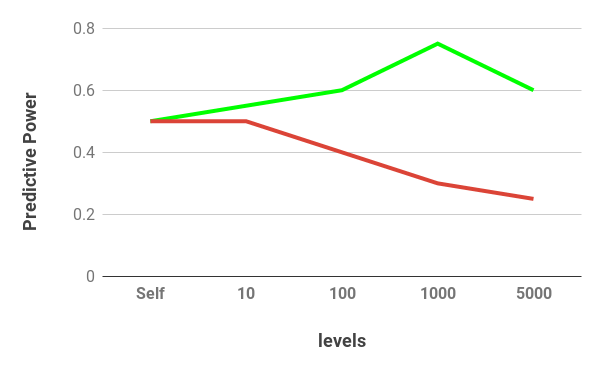
\includegraphics[width=\linewidth]{figs/predictive_power.png}
    \caption{Two hypothetical results about how training set size might effect the efficacy of quality prediction for software projects.}
    \label{fig:predictive_power}
\end{figure}

Petersen and Wohlin~\cite{Petersen2009} argue that for empirical SE, context matters.That is, they would predict that one model  will NOT  cover all  projects and that tools that report  generality  over many software projects need to also know the {\em communities} within which those conclusions   apply. Hence, this work divides into (a)~automated methods for finding sets of projects in the same {\em community}; and (b)~within each {\em community}, find the model what works best. 

The {\em size} of the communities found in this way would have a profound impact on how we should reason about software engineering. Consider the hypothetical results of Figure~\ref{fig:predictive_power}. The \textcolor{ao(english)}{{\bf GREEN}} curve shows some quality predictor that (hypothetically) gets better, the more projects it learns from (i.e. higher levels in the hierarchical cluster). After about 2 levels, the \textcolor{ao(english)}{{\bf GREEN}} curve's growth stops and we would say that community size here was around cluster size in level 1. In this case, while we could not offer a single model that cover {\em all} of SE, we could offer a handful of models, each of which would be relevant to project clusters in that level. Accordingly, we would say that there are many cases where  wisdom from prior projects can be readily applied to guide future projects and (b)~the generality issues raised are not be so pressing.

Now consider the hypothetical \textcolor{red}{{\bf RED}} curve of Figure~\ref{fig:predictive_power}. Here, we see that (hypothetically)  learning from more projects makes quality predictions worse which means the our 10,000 projects break up into ``communities'' of size one. In this case,  (a)~principles about what is ``best practice'' for different software projects would be constantly change (whenever we jump from small community to small community); and (b)~the generality issues would be become open and urgent concerns for the SE analytics community.


\subsection{Related Work}
\label{sec:related}

In this section, we ask ``Why even bother to transfer lessons learned between projects?''. In several recent studies ~\cite{bettenburg2012think, menzies2012local, posnett2011ecological} with readily-available data from SE repositories, numerous authors report the locality effect in SE; i.e. general models outperformed by specialized models localized to particular parts of the data. Menzies et al. showed in their paper about local vs global learning in defect prediction and effort estimation domain that using a rule based learner locality based learning was much effective then rules learned from the global dataset. While Herbold et al.~\cite{herbold2017global} in their study regarding global vs local model for cross-project defect prediction showed evident proof that local models make only a minor difference in comparison to global models. While local can cause conclusion instabilities, global models can miss details which is specific to certain dataset. So in this study, we review the evidence that if it is useful to explore more than just the local data. This evidence falls into four groups:

\textbf{(a) The lesson on big data is that that the {\em more} training data, the {\em better} the learned model.} Vapnik~\cite{vapnik14} discusses examples where models accuracy improves to nearly 100\%, just by training on $10^2$ times as much data. This effect has yet to be seen in SE data~\cite{menzies2013guest} but that might just mean we have yet to use enough training data (hence, this study). 

\textbf{(b) We need to learn from more data since there is very little agreement on what has been learned to far:} Another reason to try generalizing across more SE data is that, among developers, there is little agreement on what many issues relating to software:
\bi
    \item
    According to Passos et al.~\cite{passos11},  developers often  assume that the lessons they learn from a few past projects are general to all their future projects. They comment, ``past experiences were taken into account without much consideration for their context'' ~\cite{passos11}. 
	\item
	J{\o}rgensen \& Gruschke~\cite{Jo09} offer a similar warning. They report that the suppose software engineering ``gurus'' rarely use lessons from past projects to improve their future reasoning and that such poor past advice can be detrimental to new projects.~\cite{Jo09}.
    \item 
    Other studies have shown some widely-held views are   now questionable given new evidence. Devanbu et al. examined responses from 564 Microsoft software developers from around
	the world. They comment programmer beliefs can vary with each project, but do not necessarily
	correspond with actual evidence in that project~\cite{De16}. 
\ei
	
The good news is that, using software analytics, we can correct the above misconceptions. If data mining shows that doing  XYZ is bug prone, then we could  guide developers to avoid XYZ. But will developers listen to us? If they ask ``are we sure  XYZ causes problems?'', can we say that we have mined enough projects to ensure that XYZ is problematic? 

It turns out that developers are not the only ones confused about how various factors influence software projects. Much recent research calls into question  the``established widoms'' of SE field. For example, here is a list of recent conclusions that contradict prior conclusions:

\bi

    \item In stark contrast to  much prior research, pre- and post- release failures are not connected~\cite{fenton2000quantitative};
    
    \item Static code analyzers perform no better than simple statistical predictors~\cite{Fa13}; 
    
    \item The language construct GOTO, as used in contemporary practice, is rarely considered harmful~\cite{nagappan2015empirical};
    
    \item Strongly typed languages are not associated with successful projects~\cite{ray2014large};  
    
    \item Test-driven development is not any better than "test last"~\cite{fucci2017dissection};
    
    \item Delayed issues are not exponentially more expensive to fix~\cite{menzies2017delayed};

\ei

Note that if the reader disputes any of the above, then we ask how would you challenge the items on this list? Where would you get the data, from enough projects, to   successfully refute the above? And where would you get that data? And how would you draw conclusions from that large set?

\textbf{(c) Imported data can be more useful than local data:} Another benefit of  importing data from other projects is that, sometimes, that imported data can be better than the local information. For example, Rees-Jones reports in one study that while building predictors
for Github close time  for open source projects~\cite{rees2017better} using data from other projects performs much better then building models using {\em local learning} (because there is better  information {\em there} than {\em here}).


\textbf{(d) When there is insufficient local data, learning from other projects is very useful:} When developing new software in  novel areas, it is useful to draw on the relevant  experience  from related areas with a larger experience base.This is particularly true when developers are doing something that is novel to them, but has been widely applied elsewhere
For example, Clark and Madachy~\cite{clark15} discuss 65 types of software they see        under-development by the US Defense Department in 2015.   Some of these types are very common (e.g. 22 ground-based communication systems) but other types are very rare (e.g. only  one avionics communication system). (e.g. workers on   flight avionics   might check for lessons learned from ground-based communications). Developers  working in an uncommon area (e.g. avionics communications) might want to transfer in lessons from more common areas (e.g. ground-based communication).


This fuels the art of moving data and/or lessons learned from one project or another is Transfer Learning. This is when there is insufficient data to apply data miners to learn defect predictors, transfer learning can be used to transfer lessons learned from other source projects S to the target project T .

Initial experiments with transfer learning offered very pessimistic results. Zimmermann et al.~\cite{zimmermann2009cross} tried to port models between two web browsers (Internet Explorer and Firefox) and found that cross-project prediction was still not consistent: a model built on Firefox was useful for Explorer, but not vice versa, even though both of them are similar applications. Turhan's initial experimental results were also very negative: given data from 10 projects, training on S = 9 source projects and testing on T = 1 target projects resulted in alarmingly high false positive rates (60\% or more). Subsequent research realized that data had to be carefully sub-sampled and possibly transformed before quality predictors from one source are applied to a target project. Transfer learning can be have two variants - 

\bi
    \item \textbf{Homogeneous Transfer Learning:} This kind of transfer learning operates on source and target data that contain the same attributes.
    
    \item \textbf{Heterogeneous Transfer Learning:} This type of transfer learning operates on source and target data that contain the different attributes.
\ei

Another way of to divide transfer learning is the approach that is followed. There are  2 approaches that is frequently used in many research  - 

\bi
    \item \textbf{Similarity Based Approach:} In this approach we can transfer some/all subset of the rows or columns of data from source to target. For example, the Burak filter~\cite{turhan09} builds its training sets by finding the k = 10 nearest code modules in S for every $ t \in T $. However, the Burak filter suffered from the all too common instability problem (here, whenever the source or target is updated, data miners will learn a new model since different code modules will satisfy the k = 10 nearest neighbor criteria). Other researchers ~\cite{kocaguneli2012, kocaguneli2011find} doubted that a fixed value of k was appropriate for all data. That work recursively bi-clustered the source data, then pruned the cluster sub-trees with greatest ``varianc'' (where the ``variance'' of a sub-tree is the variance of the conclusions in its leaves). This method combined row selection with row pruning (of nearby rows with large variance). Other similarity methods~\cite{Zhang16aa} combine domain knowledge with automatic processing: e.g. data is partitioned using engineering judgment before automatic tools cluster the data. To address variations of software metrics between different projects, the original metric values were discretized by rank transformation according to similar degree of context factors.
    
    \item \textbf{Dimensionality Transformation Based Approach:} In this approach we manipulate the raw source data until it matches the target. An initial attempt on performing transfer learning with Dimensionality transform was undertaken by Ma et al.~\cite{Ma2012} with an algorithm called transfer naive Bayes (TNB). This algorithm used information from all of the suitable attributes in the training data. Based on the estimated distribution of the target data, this method transferred the source information to weight instances the training data. The defect prediction model was constructed using these weighted training data. Nam et al.~\cite{Nam13} originally proposed a transform-based method that used TCA based dimensionality rotation, expansion, and contraction to align the source dimensions to the target. They also proposed a new approach called TCA+, which selected suitable normalization options for TCA, When there are no overlapping attributes (in heterogeneous transfer learning) Nam et al.~\cite{Nam2015} found they could dispense with the optimizer in TCA+ by combining feature selection on the source/target following by a Kolmogorov-Smirnov test to find associated subsets of columns. Other researchers take a similar approach, they prefer instead a canonical-correlation analysis (CCA) to find the relationships between variables in the source and target data~\cite{jing2015heterogeneous}.
\ei

Considering all the attempts at transfer learning sampled above, suggested a surprising lack of consistency in the choice of datasets, learning methods, and statistical measures while reporting results of transfer learning. This issue was addressed by ``Bellwether'' suggested by Krishna et al. ~\cite{krishna2017simpler,krishna16}. which is a simple transfer learning technique is defined in 2- folds namely the Bellwether effect and the Bellwether method:

\bi

    \item \textbf{The Bellwether effect} states that, when a community works on multiple software projects,  then there exists one exemplary project, called the bellwether, which can define predictors for the others.
    
    \item \textbf{The Bellwether method} is where we search for the exemplar bellwether project and construct a transfer learner with it. This transfer learner is then used to predict for effects in future data for that community.

\ei

In their paper Krishna et al. performs experiment with communities of 3, 5 and 10 projects in each, and shows that bellwethers are not rare, their prediction performance is better than local learning, they do fairly well when compared with State of the Art transfer learning methods discussed above and with selection of bellwether shows a consistency for choice of source dataset for transfer learning. This motivated us to use ``Bellwether'' as our choice of method for transfer learning to search for generality in SE datasets. But as per Krishna et al. in order to find bellwether we need to do a $ N*(N-1) $ comparison which is order of $ N^2 $ (N being the number of projects in community). This indeed a very expensive computation. This motivated our study to find generality in SE datasets using a faster Bellwether method. 

Include details about BIRCH and effect of clustering and talk about divide and conquer. 

\section{Data Collection}
\label{sec:Data Collection}

\subsection{Data}
\label{sec:data}

To perform our experiments we choose to work with defect prediction datasets. We use data collected by zhang et al.~\cite{zhang15}. The original data was initially collected by Mockus et al.~\cite{mockus2009amassing} from SourceForge and GoogleCode and was updated till 2010. The dataset contains the full history of about 154K projects that are hosted on SourceForge and 81K projects that are hosted on GoogleCode to the date they were collected. In the original dataset each file contained the revision history and commit logs linked using a unique identified. Although there were 235K projects in the original database, we know from previous literature surveys and experience there were many trivial and non-software development projects. zhang et al. cleaned the dataset using 5 different criteria which resulted in 1385 projects being selected in the final datasets. As part of this experiment we also included few filters to select a subset of 1385 projects, which are useful for our experiment. This eventually gave us a dataset of 697 projects. The filters applied to filter out trivial projects are - 

\bi

    \item \textbf{Programming Languages:} Filtering Out Projects by Programming Languages(only object-oriented i.e *.c, *.cpp, *.cxx, *.cc, *.cs, *.java, and *.pas). This was done as the dataset was collected using a commercial tool, called Understand~\cite{visualize}(which supports the object oriented programming languages) , to compute code metrics. 

    \item \textbf{Projects with a Small Number of Commits:} As small number of commits can mean the projects do not follow a proper SE development process or they are very new, also small number of commits can not provide enough information for computing process metrics and mining defect data. Thus zhang et al. removed any projects with less than 32 commits(25 \% quantile of the number of commits as the threshold).
    
    \item \textbf{Projects with Lifespan Less Than One Year:} zhang et al. collected data in the six-months period using a split date from the first commit and compute process metrics using the change history in the six-months period before the split date. For this reason projects with a lifespan less than one year were filtered out.
    
    \item \textbf{Projects with Limited Defect Data:} For this study defect data was mined using commit messages and bug tracking reports. zhang et al. in their study counted the number of fix-inducing and non-fixing commits from a one-year period and used 152 and 1,689 commits for fix-inducing and non-fixing  respectively for SourceForge. Similarly  92 and 985 commits for GoogleCode. This number was decided by calculating the 75 \% quantile of the number of fix-inducing and non-fixing commits.
    
    \item \textbf{Projects Without Fix-Inducing Commits:} zhang et al. filtered out projects that have no fix-inducing commits during six months as abnormal projects, as projects in defect prediction studies need to contain both defective and non-defective commits.
    
    \item \textbf{Projects with less than 50 rows:} We removed any project with less than 50 rows as they are too small to build a meaningful predictor. 

\ei

\begin{figure}
    \centering
    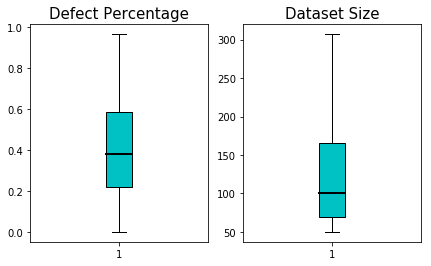
\includegraphics[width=\linewidth]{figs/meta.png}
    \caption{Two hypothetical results about how training set size might effect the efficacy of quality prediction for software projects.}
    \label{fig:meta}
\end{figure}


Along with above filtering criteria, there were few projects which didn't have enough fix-inducing vs non-fixing data points to to create a stratified k=5 fold cross-validation and we removed those projects from the final datasets. These criteria culled 99\% of projects by zhang et al. and culled 54\% of the remaining by our criteria, thus resulted in 697 projects in the final dataset.

From these selected projects, the data was labeled using issue tracking system and commit messages. If a project used issue tracking system for maintaining issue/defect history the data was labeled using that. But as per zhang et al. 42\% of the projects didn't not used issue tracking systems. For these projects labels were created analyzing commit messages by tagging them as fix-inducing commit if commit message matches the following regular expression - 

\begin{center}
\textit{(bug |fix |error |issue |crash |problem |fail |defect |patch)}
\end{center}
 

\subsection{Metric Extraction}
\label{sec:Metric Extraction}

For building any defect predictor we rely on software metrics. Software metrics can be categorized into 3 types according to Xenos \cite{Xenos} distinguishes software metrics as  follows (a) {\em Product metrics} are metrics that are directly related to the product itself, such as code statements, delivered executable, manuals, and strive to measure product quality, or attributes of the product that can be related to product quality. (b) {\em Process metrics} focus on the process of software development and measure process characteristics, aiming to detect problems or to push forward successful practices. Lastly, (c) {\em personnel metrics} (a.k.a. {\em resource metrics}) are those related to the resources required for software development and their performance. The capability, experience of each programmer and communication among all the programmers are related to product quality \cite{wolf2009predicting,de2004sometimes,cataldo2013coordination,cataldo2007coordination}. zhang et al. selected and calculated 21 product and 5 process metrics to build their universal defect prediction model, we will be using the same set of metrics for our study. The product metrics are computed by the Understand tool~\cite{visualize} using the files from the snapshot on the split date of 6 months. The process metrics are computed using the change history in the six-months period before the split date my manual collection of data using scripts. The metrics used in this study are described in table~\ref{tbl:metric}.

\small{
\begin{table}[]
\caption{List of software metrics used in this study}
\label{tbl:metric}
\scriptsize
\begin{tabular}{|p{1cm}|c|l|p{3cm}|}
\hline
\multicolumn{1}{|l|}{Metric}        & \multicolumn{1}{l|}{Metric level} & Metric Name & Metric Description             \\ \hline
\multirow{21}{*}{Product   } & \multirow{6}{*}{File}             & LOC         & Lines of Code                  \\ \cline{3-4} 
                                  &                                   & CL          & Comment Lines                  \\ \cline{3-4} 
                                  &                                   & NSTMT       & Number of Statements           \\ \cline{3-4} 
                                  &                                   & NFUNC       & Number of Functions            \\ \cline{3-4} 
                                  &                                   & RCC         & Ratio Comments to Code         \\ \cline{3-4} 
                                  &                                   & MNL         & Max Nesting Level              \\ \cline{2-4} 
                                  & \multirow{12}{*}{Class}           & WMC         & Weighted Methods per Class     \\ \cline{3-4} 
                                  &                                   & DIT         & Depth of Inheritance Tree      \\ \cline{3-4} 
                                  &                                   & RFC         & Response For a Class           \\ \cline{3-4} 
                                  &                                   & NOC         & Number of Immediate Subclasses \\ \cline{3-4} 
                                  &                                   & CBO         & Coupling Between Objects       \\ \cline{3-4} 
                                  &                                   & LCOM        & Lack of Cohesion in Methods    \\ \cline{3-4} 
                                  &                                   & NIV         & Number of instance variables   \\ \cline{3-4} 
                                  &                                   & NIM         & Number of instance methods     \\ \cline{3-4} 
                                  &                                   & NOM         & Number of Methods              \\ \cline{3-4} 
                                  &                                   & NPBM        & Number of Public Methods       \\ \cline{3-4} 
                                  &                                   & NPM         & Number of Protected Methods    \\ \cline{3-4} 
                                  &                                   & NPRM        & Number of Private Methods      \\ \cline{2-4} 
                                  & \multirow{3}{*}{Methods}          & CC          & McCabe Cyclomatic Complexity   \\ \cline{3-4} 
                                  &                                   & FANIN       & Number of Input Data           \\ \cline{3-4} 
                                  &                                   & FANOUT      & Number of Output Data          \\ \hline
\multirow{5}{*}{Process }  & \multirow{5}{*}{File}             & NREV        & Number of revisions            \\ \cline{3-4} 
                                  &                                   & NFIX        & Number of revisions a file     \\ \cline{3-4} 
                                  &                                   & ADDED LOC    & Lines added                    \\ \cline{3-4} 
                                  &                                   & DELETED LOC  & Lines deleted                  \\ \cline{3-4} 
                                  &                                   & MODIFIED LOC & Lines modified                 \\ \hline
\end{tabular}
\end{table}
}


\section{Experimental Setup}
\label{sec:Experimental}

In this study we try to establish the presence of generality in SE datasets. We do this by analyzing the presence of bellwether incrementally by adding more and more projects and how the bellwether's predictive power changes. In this case to show the presence of generality in SE datasets the predictive power of the bellwether should look like the \textcolor{ao(english)}{GREEN} in figure~\ref{fig:predictive_power}, that is the predictive power of bellwether should increase or remains same, if our results look like the \textcolor{red}{RED} curve, that will show absence of generality in SE datasets.

In order to achieve this we try to explore the \textit{bellwether effect} as mentioned in ~\ref{sec:related}. We know the default \textit{bellwether method} is very expensive ($ O(N^2) $). Thus in this paper we proposes an alternative transfer learning method (BUBBLE), that explores \textit{bellwether effect} by exploring an order of magnitude faster \textit{bellwether method}. Our approach has three key components:

\bi

    \item A feature extractor to find a representation of each project, which will be used for clustering the projects. 
    
    \item A hierarchical clustering model to use the features extracted from previous step to build the hierarchical cluster.
    
    \item A transfer learning model to identify bellwether in the hierarchical cluster.

\ei

BUBBLE employs few different algorithms to complete and compose it's 4 different components - 

\subsection{Feature Subset Selection (FSS)}
\label{subsec:FSS}
To extract features from each dataset, we use a feature selector algorithm called Feature Subset Selection(FSS)~\cite{hall1999correlation,hall1997feature}. Which is a process of identifying and removing as much irrelevant and redundant information as possible. This is achieved using a correlation based feature evolution strategy to evaluate importance of an attribute and a best first search strategy with back tracking that moves through the search space by making local changes to the current feature subset.Here if the path being explored begins to look less promising, the best first search can back-track to a more promising previous subset and continue the search from there. Given enough time, a best first search will explore the entire search space, so it uses a stopping criterion (i.e. no improvement for five consecutive attributes). XXX

\small{
\begin{figure}[]
    \small
     \begin{lstlisting}[mathescape,linewidth=7.5cm,frame=none,numbers=right]
      def CFS(data):
        features = []
        score = -0.000000001
        while True:
            best_feature = None
            for feature in range(data.features):
                features.append(feature)
                temp_score = calculate_corr(data[F])
                if temp_score > score:
                    score = temp_score
                    best_feature = features
                features.pop()
            features.append(best_feature)
            if not improve(score):
                break
        return features
    
    \end{lstlisting} 
    \vspace{-0.2cm}
    \caption{Pseudo-code of Feature Subset Selection}
    \label{fig:GAP_pseudocode} 
    \vspace{-0.3cm}
\end{figure}
}
\subsection{Balanced Iterative Reducing and Clustering using Hierarchies (BIRCH)}
\label{subsec:BIRCH}
To find presence or absence of generality in SE datasets, we need to incrementally check for ``Bellwether'' from smaller to larger community. A community is a set of project which is similar in nature. We use the BIRCH algorithm on our defect prediction dataset to create a hierarchical clustering tree to form these communities. BIRCH~\cite{zhang1996birch} is  a hierarchical clustering algorithm, which has a ability to incrementally and dynamically cluster incoming, multi-dimensional data in an attempt to produce the best quality clustering. BIRCH also has the ability to identify data points that are not part of the underlying pattern effectively identifying outliers. In this study we uses a modified BIRCH algorithm to store additional information regarding each cluster in the clustering feature tree, which help us in the experiment. XXX

\subsection{Synthetic Minority Over-Sampling Technique (SMOTE)}
\label{subsec:SMOTE}

Machine learning models exploits the inherent bias in the dataset to segregate and classify different classes. Hence class imbalance can create major bias towards the majority class when building a machine learning model, thus producing biased model which provides bad classification results. Synthetic Minority Over-Sampling Technique (SMOTE)~\cite{chawla2002smote} is a technique to handle class imbalance by changing the frequency of different classes of the training data. When applied to data, SMOTE sub-samples the majority class (i.e., deletes some examples) while over-sampling the minority class until all classes have the same frequency. In the case of software defect data, the minority class is usually the defective class. During super-sampling, a member of the minority class finds k nearest neighbors. It builds an artificial member of the minority class at some point in-between itself and one of its random nearest neighbors. During that process, some distance function is required which is the \textit{minkowski distance} function.

\subsection{Logistic Regression (LR)}
\label{subsec:LR}

Logistic regression is a statistical machine learning model that in its basic form uses a logistic function to model a binary dependent variable. In this study we use scikit learn's default logistic regression implementation as our learner for building source models and evaluating on target models inside each community. In this study we selected logistic regression, as it is very fast to build in comparison to other more complex learners and its much more comprehensible and explainable in-terms of attributes and their importance. Logistic Regression is widely used in defect prediction domain and have shown promising results both in-term of predictive power and comprehensibility.


\subsection{Bellwether\_0:}
\label{Bellwether}

In this study to compare our novel method to the state of the art method, we uses Krishna et al. 's \textit{bellwether method}. We use all the projects available in the community to perform a $N*(N-1)$ comparison, where N is the number of projects in the community to measure the performance of each project measured on all others on the performance measures mentioned in sec~\ref{sec:Measures}. Following this we use cdom function to select a bellwether project among them. 



\subsection{BUBBLE}
\label{BUBBLE}

BUBBLE is a \textit{bellwether method} algorithm which combines the components described above, to create a fast way to find \textit{bellwether effect}. BUBBLE works in 6 stages - 

    (1) \textbf{Feature Extraction:} In this stage the whole dataset is used to extract feature from each projects. This is done using the FSS algorithm as shown in~\ref{subsec:FSS}. Here each project is sent to the FSS and the FSS returns most suitable features for building models, we do this for every project and that information as a vector (i.e. a vector or length equal to total number of features, where 1 represents a feature being selected ,0 is the other way around) that represents each project. By performing this we have a vector representation of each project in the dataset. BUBBLE uses this information to create the hierarchical clusters to find the communities. We perceive this is a good representation of community, as in this work we try to find community which has similar information distribution according to the attributes. Thus 2 projects with similar features selected have much higher chance of building similar models.
    
    (2) \textbf{Cluster Creation:} After the feature extraction has been done, the data is sent to a modified BIRCH algorithm. The algorithm requires a branching factor (i.e. Maximum number of CF sub-clusters in each node) and threshold value (i.e. when to form a new cluster based on radius). For this experiment we have set the branching factor as 20 and threshold value as 0.5. Using this version of BIRCH algorithm we build the hierarchical cluster, while storing all necessary details about the cluster like parent-child node, data points, level information etc. This stage returns a Clustering Feature Tree (CF Tree) with all those information, which is passed to the next phase of experiment. 
    
    (3) \textbf{Bellwether selection phase 1:} The CF Tree from the last phase is passed to the hierarchical bellwether. In this phase we use \textit{bellwether method} to identify bellwether at the leaf level. Using the CF Tree, we identify the clusters at the leaf level where each cluster represents the smallest community produced by the BIRCH algorithm in the last phase. Here we use the default ``Bellwether'' to perform a $ N*(N-1) $ comparison at each cluster.Here we select each project in the cluster one by one as a source dataset for transfer learning apply SMOTE as mentioned in sec~\ref{subsec:SMOTE} to handle any data imbalance and then use the FSS algorithm to get rid of any unnecessary attributes as mentioned in sec~\ref{subsec:FSS}. This informative and balanced dataset is used to build a LR model as mentioned in sec~\ref{subsec:LR} and we measure the performance of all other projects in the community(cluster). The performance measures that are used are mentioned in sec~\ref{sec:Measures}. To find the bellwether in each community we use cdom function to find the best source dataset among each cluster considering all performance measures. This phase returns a bellwether for each cluster at the leaf level of the CF Tree.
    
    (4) \textbf{Bellwether promotion:} In this phase of the algorithm is an iterative process, here we receive the selected bellwethers from the child clusters of each cluster in the level. This is called the bellwether promotion. Here each parent cluster instead of being represented by all projects within them, they are represented by only the bellwethers in them.  
    
    (5) \textbf{Bellwether selection phase 2:} In this phase instead of finding a bellwether for each cluster at the level by performing a $ N*(N-1) $ comparison, we select the projects which represented as bellwether at the child nodes and then try to find a bellwether among them. So at each cluster at the level we perform a a $ M*(M-1) $ comparison at each cluster where M is the selected bellwether from child clusters. This creates a order of magnitude faster \textbf{bellwether method}. This is again an iterative process, and the end of all the iterations, we will have a bellwether at each cluster at every level. 
    
    (6) \textbf{Bellwether Prediction:} This is the transfer learning phase, when a new project is to evaluated we will use the FSS algorithm to get its features, then use the feature vectors to identify which cluster it belongs and use that cluster's bellwether as the transfer learning model.


To report the finding and results of this study without any bias, we repeat the experiment 20 times by dividing the dataset randomly into train\_1 and test\_1 as a 90-10 split, the projects in train\_1 was used to find the bellwether in each cluster in the CF Tree, and then each project in test\_1 was divide into train\_2 and test\_2 split. We trained a LR model using train\_2 for each project and tested on test\_2, this is represented as self test in this study. We also used the predict stage of the BUBBLE to identify bellwether for each project in test\_1 and tested the performance on test\_2. 


\small{
\begin{figure}[]
    \small
     \begin{lstlisting}[mathescape,linewidth=7.5cm,frame=none,numbers=right]
      def BUBBLE(data):
        project_features = get_features(data)
        cluster_tree = BIRCH(project_features)
        bellwethers = h_bellwether(cluster_tree)
        for project in test_1:
            train_2,test_2 = train_test_split(data[project])
            self_clf = LR(train_2)
            b_clf = find_bellwether(project_features[project])
            self_score = self_clf.predict(test_2)
            bellwether_score = b_clf.predict(test_2)
            results.append([self_score,bellwether_score]) 
        return results
    \end{lstlisting} 
    \vspace{-0.2cm}
    \caption{Pseudo-code of BUBBLE Experiment}
    \label{fig:GAP_pseudocode} 
    \vspace{-0.3cm}
\end{figure}
}

\small{
\begin{figure}[]
    \small
     \begin{lstlisting}[mathescape,linewidth=7.5cm,frame=none,numbers=right]
      def h_bellwether(cluster_tree):
        bellwethers = { }
        def bellwether(list1,list2):
            for source in list1:
                clf = LR(source)
                _list2 = list2.pop(source)
                for dest in _list2:
                    score[source][dest] = clf.predict(dest)
            return best(score.key())
        for level in cluster_tree.levels:
            if level == cluster_tree.max_level:
                for c in cluster_tree[level].clusters:
                    bellwethers[c] = bellwether(c.projects,
                                                c.projects)
            else:
                for c in cluster_tree[level].clusters:
                    child_clusters = c.child
                    _bellwethers = bellwethers[child_clusters]
                    bellwethers[c] = bellwether(_bellwethers,
                                                _bellwethers)
        return bellwethers
    \end{lstlisting} 
    \vspace{-0.2cm}
    \caption{Pseudo-code of Hierarchical Bellwether}
    \label{fig:GAP_pseudocode} 
    \vspace{-0.3cm}
\end{figure}
}

\subsection{Statistical Tests}
\label{stats}

When comparing the results different models in this study, we used a statistical significance test and an effect size test. Significance test are useful for detecting if two populations
differ merely by random noise. Also, effect sizes are useful for checking that two populations differ by more than just a trivial amount. For the significance test,  we use the Scott-Knott procedure  recommended at TSE'13~\cite{mittas2013ranking} and ICSE'15~\cite{ghotra2015revisiting}. This technique recursively bi-clusters a sorted set of numbers. If any two clusters are statistically indistinguishable, Scott-Knott reports them both as one group. Scott-Knott first looks for a break in the sequence that maximizes the expected values in the difference in the means before and after the break.More specifically,  it  splits $l$ values into sub-lists $m$ and $n$ in order to maximize the expected value of differences  in the observed performances before and after divisions. For e.g., lists $l,m$ and $n$ of size $ls,ms$ and $ns$ where $l=m\cup n$, Scott-Knott divides the sequence at the break that maximizes:

\begin{equation}
    E(\Delta)=ms/ls*abs(m.\mu - l.\mu)^2 + ns/ls*abs(n.\mu - l.\mu)^2\
\end{equation}

Scott-Knott then applies some statistical hypothesis test $H$ to check if $m$ and $n$ are significantly different. If so, Scott-Knott then recurses on each division. For this study, our hypothesis test $H$ was a conjunction of the A12 effect size test (endorsed by \cite{arcuri2011practical})  and non-parametric bootstrap sampling \cite{efron94}, i.e., our Scott-Knott divided the data if {\em both} bootstrapping and an effect size test agreed that the division was statistically significant (90\% confidence) and not a ``small'' effect ($A12 \ge 0.6$).

\subsection{Continuous Domination(cdom)}
\label{cdom}
In this study, we compare each project's performance against all other projects in each cluster at the leaf level of the BIRCH as described in section~\ref{BUBBLE} and section~\ref{Bellwether}. We calculate 5 different performance measure for each project as described in section~\ref{sec:Measures}. In order to find a \textit{bellwether effect} in the performances collected we need to combine those 5 performance measures and then rank them using certain criteria. We have used continuous domination (cdom) for this purpose. continuous domination is defined as the set of all points in the objective space that are not dominated by any other points. Unlike Boolean domination, which says a point is dominated by another if and only if the first point is better in every single objective then the second point, continuous domination combines all the objective into a continuous function to compare and then calculate if one point dominates another. Throughout literature continuous domination has proven to be very effective when multiple goals are concerned. The continuous domination function is defined as below, where P is the total population, k is fitness scaling factor and $X\_1$ is the data points we are calculating the domnation for - 

\begin{equation}
    F(X_1) = \sum_{{(X_2\in P) - X_1}} -e^{-I(X_2,X_1)/k}
\end{equation}


\section{Performance Measures}
\label{sec:Measures}

In this section, we introduce the following 5 evaluation measures used in this study to evaluate the performance of machine learning models. Suppose we have a dataset with M changes and N defects. After inspecting 20\% LOC, we inspected m changes and found n defects. Besides, when we find the first defective change, we have inspected k changes. Then the 5 evaluation measures are defined and computed as follows:

(1) \textbf{Recall:} Proportion of inspected defective changes among all the actual defective changes. This is the evaluation measure used by many previous studies~\cite{kamei2012large,yang2016effort,yang2017tlel,xia2016collective,yang2015deep} . They focused on achieving high Recall so that more defective changes could be detected. Recall is computed as: $n/N$.

(2) \textbf{Precision:} Proportion of inspected defective changes among all the inspected changes. A low Precision indicates that developers would encounter more false alarms, which may have negative impact on developers' confidence on the prediction model. Precision is computed as: $n/m$.

(3) \textbf{pf:} Proportion of all suggested defective changes which are not actual defective changes among all the suggested defective changes. A high pf suggests developers will encounter more false alarms which may have negative impact on developers' confidence on the prediction model.

(4) \textbf{popt20:} Proportion number of suggested defective changes among all suggested defective changes, when when 20\% LOC modified by all changes are inspected. A high popt20 indicates that, under the same number of LOC to inspect, developers developers will find more bugs, which means developers will be able to fix more defects with same amount of effort invested. XXX

(5) \textbf{ifa:} Number of Initial False Alarms encountered before we find the first defect. Inspired by previous studies on fault localization~\cite{parnin2011automated,kochhar2016practitioners,xia2016automated}, we assume that if the top-k changes recommended by the model are all false alarms, developers would be frustrated and are not likely to continue inspecting the other changes. For example, Parnin and Orso ~\cite{parnin2011automated} investigated how developers use and benefit from automated debugging tools through a set of human studies. They found that developers would stop inspecting suspicious statements, and turn back to traditional debugging, if they could not get promising results within the first few statements they inspect. ifs is computed as: k.


\section{Results}
\label{sec:results}

\subsection{RQ1: Can we confirm bellwether on large datasets?}
\label{sec:rq1}

In the literature, we saw most of the previous studies has shown bellwether effect with very small datasets. In order to use bellwether to prove presence of generality in SE domain datasets, we first have to showcase the bellwether method suggested by Krishna et al. in their experiment works for large datasets. We use our defect prediction dataset with 697 projects for this purpose. We divide the dataset in train\_1 and test\_1 set and then performed a $ N*(N-1) $ comparison on all the projects in train\_1 set to find a bellwether, and then dividing each project in test\_1 set into train\_2 and test\_2 using a train\_test split. We use the train\_2 to train a LR model and test on test\_2 which is represented as \textit{self\_0} in the figures. Similarly we use the bellwether project from train\_1 to train a LR model and test it on test\_2 which is represented as \textit{bellwether0}. We use statistical tests mentioned in section~\ref{stats} to compare the performance of \textit{self\_0} vs \textit{bellwether0} for all the performance measures mentioned in section~\ref{sec:Measures}, which is shown in figure~\ref{fig:recall}, \ref{fig:precision}, \ref{fig:pf}, \ref{fig:popt20}, \ref{fig:ifa} . It is evident that using the \textit{bellwether method} proposed by Krishna et al. we were able to find bellwether effect in large dataset with 697 projects. This answers this RQ and creates the baseline results for our study. In this RQ1 although we are able to find \textit{bellwether effect}, this method is very expensive, requiring a $ N*(N-1) $ comparison, which in our experimental setup took nearly 75 days of computation on a single core machine. Which takes us to the next research question. 



\subsection{RQ2: How to tame complexity of bellwether?}
\label{sec:rq2}

To tame complexity of bellwether in this RQ, we propose a new bellwether method called ``BUBBLE'' to find bellwether in large datasets. This bellwether method is composed of 6 stages, (a) a feature extraction process to summarize each project into a single representative vector, (b) a hierarchical clustering algorithm, which uses the feature vectors to cluster similar projects into community of increasing size at different levels of cluster, (c) a bellwether selection phase where a $N*(N-1)$ comparison is performed at each leaf level cluster and using a cdom calculation in all the metrics mentioned in~\ref{tbl:metric} a bellwether is selected, (d) a iterative bellwether promotion stage, where bellwether from child clusters are promoted as potential bellwethers at parent cluster, (e) another bellwether selection phase at non-leaf levels, where comparisons are only made among potential bellwethers from leaf node and finally (f) a bellwether prediction phase, which suggests a bellwether based on project similarity when a new project is to be predicted. The details of each phase is mentioned in sec~\ref{BUBBLE}. 

In the \textit{bellwether method} proposed by Krishna et al. if there are N projects in a community it will make $\approx N^2$ comparisons to discover the bellwether. While ``BUBBLE'' different approach to discover bellwether by dividing the data into smaller cluster and finding bellwether among each, here if we assume we have m cluster at leaf level with N projects in each, we will have 
$\approx N^2/m$ comparisons to discover the bellwether which is m times less comparison. Using this process we able to find bellwether in ~1.5 hours, which is order of magnitude faster then the bellwether method proposed by Krishna et al. 

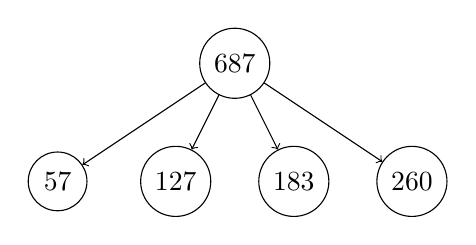
\begin{tikzpicture}[nodes={draw, circle}, ->]
 
    \node{687}
        child { node {57} }
        child { node {127} }
        child { node {183} }
        child { node {260} };
 
\end{tikzpicture}



%%%%%%%%%%%%%%%%%%%%%%%%%%%%%%%%%%%%%%%%%%%%%%%%%%%%%%%%%%%
%%%%%%%%%%%%%%%%%%%%%%%Latex Table%%%%%%%%%%%%%%%%%%%%%%%%%
\begin{figure}[!t]
{\small
{\small \begin{tabular}{llrrc}
\arrayrulecolor{darkgray}
\rowcolor[gray]{.9}  rank & treatment & median & IQR & \\
    1 &      self\_0 &    50 &  86 & \quart{0}{50}{86}{36} \\
    2 &      bellwether0 &    67 &  64 & \quart{36}{67}{64}{33} \\
    2 &      bellwether\_level2 &    67 &  67 & \quart{33}{67}{67}{33} \\
    2 &      bellwether\_level1 &    67 &  62 & \quart{38}{67}{62}{33} \\
    3 &      bellwether\_level0 &    78 &  50 & \quart{50}{78}{50}{22} \\
\end{tabular}}
}
\caption{Recall
}\label{fig:recall}
\end{figure}
%%%%%%%%%%%%%%%%%%%%%%%End Latex Table%%%%%%%%%%%%%%%%%%%%%
%%%%%%%%%%%%%%%%%%%%%%%%%%%%%%%%%%%%%%%%%%%%%%%%%%%%%%%%%%%

%%%%%%%%%%%%%%%%%%%%%%%%%%%%%%%%%%%%%%%%%%%%%%%%%%%%%%%%%%%
%%%%%%%%%%%%%%%%%%%%%%%Latex Table%%%%%%%%%%%%%%%%%%%%%%%%%
\begin{figure}[!t]
{\small
{\small \begin{tabular}{llrrc}
\arrayrulecolor{darkgray}
\rowcolor[gray]{.9}  rank & treatment & median & IQR & \\
    1 &      bellwether\_level0 &    43 &  47 & \quart{20}{43}{47}{24} \\
    1 &      bellwether0 &    44 &  47 & \quart{20}{44}{47}{23} \\
    1 &      bellwether\_level2 &    50 &  51 & \quart{20}{50}{51}{21} \\
    1 &      bellwether\_level1 &    50 &  51 & \quart{20}{50}{51}{21} \\
    1 &      self\_0 &    60 &  83 & \quart{0}{60}{83}{23} \\
\end{tabular}}
}
\caption{Precision
}\label{fig:precision}
\end{figure}
%%%%%%%%%%%%%%%%%%%%%%%End Latex Table%%%%%%%%%%%%%%%%%%%%%
%%%%%%%%%%%%%%%%%%%%%%%%%%%%%%%%%%%%%%%%%%%%%%%%%%%%%%%%%%%

%%%%%%%%%%%%%%%%%%%%%%%%%%%%%%%%%%%%%%%%%%%%%%%%%%%%%%%%%%%
%%%%%%%%%%%%%%%%%%%%%%%Latex Table%%%%%%%%%%%%%%%%%%%%%%%%%
\begin{figure}[!t]
{\small
{\small \begin{tabular}{llrrc}
\arrayrulecolor{darkgray}
\rowcolor[gray]{.9}  rank & treatment & median & IQR & \\
    1 &      self\_0 &    20 &  50 & \quart{0}{20}{50}{30} \\
    2 &      bellwether0 &    50 &  55 & \quart{25}{50}{55}{30} \\
    2 &      bellwether\_level2 &    50 &  54 & \quart{21}{50}{54}{25} \\
    2 &      bellwether\_level1 &    50 &  50 & \quart{25}{50}{50}{25} \\
    3 &      bellwether\_level0 &    67 &  67 & \quart{33}{67}{67}{33} \\
\end{tabular}}
}
\caption{PF
}\label{fig:pf}
\end{figure}
%%%%%%%%%%%%%%%%%%%%%%%End Latex Table%%%%%%%%%%%%%%%%%%%%%
%%%%%%%%%%%%%%%%%%%%%%%%%%%%%%%%%%%%%%%%%%%%%%%%%%%%%%%%%%%

%%%%%%%%%%%%%%%%%%%%%%%%%%%%%%%%%%%%%%%%%%%%%%%%%%%%%%%%%%%
%%%%%%%%%%%%%%%%%%%%%%%Latex Table%%%%%%%%%%%%%%%%%%%%%%%%%
\begin{figure}[!t]
{\small
{\small \begin{tabular}{llrrc}
\arrayrulecolor{darkgray}
\rowcolor[gray]{.9}  rank & treatment & median & IQR & \\
    1 &      bellwether0 &    33 &  21 & \quart{25}{33}{21}{13} \\
    1 &      self\_0 &    33 &  50 & \quart{0}{33}{50}{17} \\
    1 &      bellwether\_level2 &    33 &  20 & \quart{25}{33}{20}{12} \\
    1 &      bellwether\_level0 &    33 &  16 & \quart{27}{33}{16}{10} \\
    1 &      bellwether\_level1 &    33 &  20 & \quart{25}{33}{20}{12} \\
\end{tabular}}
}
\caption{Popt20
}\label{fig:popt20}
\end{figure}
%%%%%%%%%%%%%%%%%%%%%%%End Latex Table%%%%%%%%%%%%%%%%%%%%%
%%%%%%%%%%%%%%%%%%%%%%%%%%%%%%%%%%%%%%%%%%%%%%%%%%%%%%%%%%%


%%%%%%%%%%%%%%%%%%%%%%%%%%%%%%%%%%%%%%%%%%%%%%%%%%%%%%%%%%%
%%%%%%%%%%%%%%%%%%%%%%%Latex Table%%%%%%%%%%%%%%%%%%%%%%%%%
\begin{figure}[!t]
{\small
{\small \begin{tabular}{llrrc}
\arrayrulecolor{darkgray}
\rowcolor[gray]{.9}  rank & treatment & median & IQR & \\
    1 &      bellwether0 &    1 &  4 & \quartx{0}{1}{4}{3} \\
    1 &      self\_0 &    1 &  5 & \quartx{0}{1}{5}{4} \\
    1 &      bellwether\_level2 &    1 &  4 & \quartx{0}{1}{4}{3} \\
    1 &      bellwether\_level0 &    1 &  4 & \quartx{0}{1}{4}{3} \\
    1 &      bellwether\_level1 &    1 &  4 & \quartx{0}{1}{4}{3} \\
\end{tabular}}
}
\caption{IFA
}\label{fig:ifa}
\end{figure}
%%%%%%%%%%%%%%%%%%%%%%%End Latex Table%%%%%%%%%%%%%%%%%%%%%
%%%%%%%%%%%%%%%%%%%%%%%%%%%%%%%%%%%%%%%%%%%%%%%%%%%%%%%%%%%


\subsection{RQ3: Is faster bellwether effective?}
\label{sec:rq3}

In RQ2, we can see using ``BUBBLE'' we are able to find bellwether for a large dataset in order of magnitude faster. This raises the question is  \textit{bellwether method} ``BUBBLE'' as effective as \textit{bellwether method} proposed by krishna et al.? To answer this question in this study we have used the defect prediction dataset with 697 projects and divided the projects randomly into train\_1 and test\_1 as a 90-10 split, the projects in train\_1 was used to find the bellwether in each cluster in the CF Tree as mentioned in sec~\ref{BUBBLE}, and then each project in test\_1 was divide into train\_2 and test\_2 split. We trained a LR model using train\_2 for each project and tested on test\_2 (represented as self\_0), this is represented as self test in this study. We also used the predict stage of the ``BUBBLE'' to identify a bellwether in each level of hierarchical model, for each project in test\_1 and tested the performance on test\_2 (represented as bellwether\_level0, bellwether\_level1, bellwether\_level respectively). Similarly we used the projects in train\_1 to find the bellwether using default bellwether method as mentioned in sec~\ref{Bellwether}, and use that project to build a LR model and test the performance of each project's test\_2 (represented as bellwether0). We compare the performance of each model described above using statistical tests as mentioned in section~\ref{stats} and if 2 models are ranked different that represents their performance is significantly different. We can see from the figure~\ref{fig:recall} that bellwether\_level0 model (i.e. the bellwether discovered by ``BUBBLE'' at level 0) performs best with a median of 78 and IQR of 50. 
We can see from the results in , ~\ref{fig:precision}, ~\ref{fig:pf}, ~\ref{fig:popt20}, ~\ref{fig:ifa}. 


\subsection{RQ4: Should SE uses general methods or cohert based methods?}
\label{sec:rq4}

This RQ is about presence of generality in SE datasets based on the results from ``BUBBLE'' in RQ~\ref{sec:rq1}, RQ~\ref{sec:rq2} and RQ~\ref{sec:rq3}. 

\section{Discussion}
\label{sec:discuss}
What's old is new. Our results 

\section{Threats to Validity}
\label{sec:validity}

As with any large scale empirical study, biases can affect the final
results. Therefore, any conclusions made from this work
must be considered with the following issues in mind:

\bi 

\item \textit{Evaluation Bias}: 
In  RQ1, RQ2 and RQ3 we have shown the performance of local model, hierarchical bellwether models, default bellwether model and compared them using statistical tests on their performance to make conclusion about presence of generality in SE datasets. While those results are true, that conclusion is scoped by the evaluation metrics we used to write this paper. It is possible that, using other measurements, there may well be a difference in these different kinds of projects. This is a matter that needs to be explored in future research.  

    
\item \textit{Construct Validity}: At various places in this report, we made engineering decisions about (e.g.) choice of machine learning models, hierarchical clustering algorithm, selecting feature vectors for each r=project. While those decisions were made using advice from the literature, we acknowledge that other constructs might lead to different conclusions. 

\item \textit{External Validity}: For this study we have relied on data collected by zhang et al.~\cite{zhang15} for their studies. The metrics collected for each project was done using an commercialized tool called ``Understand''. There is a possibility that calculation of metrics or labeling of defective vs non-defective using other tools or methods may result in different outcome. That said, the ``Understand'' is a commercialized tool which has detailed documentation about the metrics calculations and zhang et al. has shared their scripts and process to convert the metrics to usable format and has described the approach to label defects.  

We have relied on issues marked as a `bug' or `enhancement' to count bugs or enhancements, and bug or enhancement resolution times. In Github, a bug or enhancement might not be marked in an issue but in commits. There is also a possibility that the team of that project might be using different tag identifiers for bugs and enhancements. To reduce the impact of this problem, we  did take precautionary step to (e.g.,) include various tag identifiers from Cabot et al.~\cite{cabot2015exploring}. We also took precaution to remove any pull merge requests from the commits to remove any extra contributions added to the hero programmer. 

\item \textit{Statistical Validity}: To increase the validity of our results, we applied two statistical tests, bootstrap and the a12. Hence, anytime in this paper we reported that ``X was different from Y'' then that report was based on both an effect size and a statistical significance test.
 
\item \textit{Sampling Bias}: Our conclusions are based on the 697 projects collected by zhang et al.~\cite{zhang15} for their studies. It is possible that different initial projects would have lead to different conclusions. That said, this sample is very large so we have some confidence that this sample represents an interesting range of projects. As evidence of that, we note that our sampling bias is less pronounced than other ``Bellwether'' studies since we explored.
 
\ei



\section{Conclusion}
\label{sec:concl}

The established wisdom in the literature is to depreciate `

\section{Future Work}
\label{sec:furute}



\section{Acknowledgements}
\label{sec:ack}

The first and second authors conducted this research study as part
of their internship at the industry in Summer, 2017. 


\balance

\bibliographystyle{ACM-Reference-Format}

\bibliography{main}
%
%\documentclass[sigconf]{acmart}
\documentclass[sigconf]{acmart} 
\pdfoutput=1
\usepackage[shortlabels]{enumitem}
\usepackage{balance}
\usepackage{dblfloatfix}

\usepackage{hyperref}
\usepackage{cleveref}
\usepackage{colortbl}
%\usepackage{color}
%\usepackage{booktabs} % For formal tables
%\usepackage{graphicx}
%\usepackage{float}
%\usepackage{listings}
%\usepackage{url}
%\usepackage{comment}
%\usepackage{multirow}
%\usepackage{rotating}
% \usepackage{bigstrut}
% \usepackage{graphics}
% \usepackage{picture}
%\usepackage{cite}

\makeatletter
\let\th@plain\relax
\makeatother


\newcommand{\bi}{\begin{itemize}[leftmargin=0.4cm]}
	\newcommand{\ei}{\end{itemize}}
\newcommand{\be}{\begin{enumerate}[leftmargin=0.4cm]}
	\newcommand{\ee}{\end{enumerate}}


\usepackage{picture}
\newcommand{\quart}[4]{\begin{picture}(100,6)%1
{\color{black}\put(#2,3){\color{red}\circle*{4}}\put(#1,3){\line(1,0){#3}}}\end{picture}}
\newcommand{\quartr}[4]{\begin{picture}(100,6)%1
{\color{black}\put(#2,3){\color{red}\circle*{4}}\put(#1,3){\line(1,0){#3}}}\end{picture}}
\newcommand{\quartx}[4]{\begin{picture}(100,1)%1
{\color{black}\put(\numexpr #2 * 6  \relax,3){\color{red}\circle*{4}}\put(\numexpr #1*6 \relax ,3){\line(1,0){\numexpr #3*6 \relax}}}\end{picture}}

\definecolor{lightgray}{gray}{0.8}
\definecolor{darkgray}{gray}{0.6}
\definecolor{Gray}{gray}{0.85}
\definecolor{Blue}{RGB}{0,29,193}

% \usepackage{tabularx}
% \usepackage{hhline}
% \usepackage[export]{adjustbox}

\definecolor{ao(english)}{rgb}{0.0, 0.5, 0.0}

\definecolor{Gray}{gray}{0.85}
\usepackage{tikz}
\usepackage{framed}
\usepackage[framed]{ntheorem}
\usepackage{multirow}
\usetikzlibrary{shadows}
\usepackage{listings}
\definecolor{MyDarkBlue}{rgb}{0,0.08,0.45} 
\lstset{
    language=Python,
    basicstyle=\sffamily\fontsize{2.5mm}{0.7em}\selectfont,
    breaklines=true,
    prebreak=\raisebox{0ex}[0ex][0ex]{\ensuremath{\hookleftarrow}},
    frame=l,
    keepspaces=false,
    showtabs=false,
    columns=fullflexible,
    showspaces=false,
    showstringspaces=false,
    keywordstyle=\bfseries\sffamily,
    emph={while, for , if ,data, def}, emphstyle=\bfseries\color{blue!50!black},
    stringstyle=\color{green!50!black},
    commentstyle=\color{red!50!black}\it,
    numbers=left,
    captionpos=t,
    escapeinside={\%*}{*)}
}

\theoremclass{Lesson}
\theoremstyle{break}

% inner sep=10pt,
\tikzstyle{thmbox} = [rectangle, rounded corners, draw=black, fill=Gray!40]
\newcommand\thmbox[1]{%
	\noindent\begin{tikzpicture}%
	\node [thmbox] (box){%
		\begin{minipage}{.94\textwidth}%
		\vspace{-0.1cm}#1\vspace{-0.1cm}%
		\end{minipage}%
	};%
	\end{tikzpicture}}

\let\theoremframecommand\thmbox
\newshadedtheorem{lesson}{Result}


% \setcopyright{none}

% % \acmDOI{10.475/123_4}
% % % ISBN
% % \acmISBN{123-4567-24-567/17/08}
% \acmConference[ICSE SEIP'18]{International Conference on Software Engineering, SE in practice track}{May 2018}{Gothenburg, Sweden} 
% \acmYear{2018}
% \copyrightyear{2018}

% \acmPrice{00.00}

%\hyphenation{op-tical net-works semi-conduc-tor}


\begin{document}
%\pagestyle{plain}

\copyrightyear{2018} 
\acmYear{2018} 
\setcopyright{acmcopyright}
\acmConference[ICSE-SEIP '18]{40th International Conference on Software Engineering: Software Engineering in Practice Track}{May 27-June 3, 2018}{Gothenburg, Sweden}
\acmBooktitle{ICSE-SEIP '18: 40th International Conference on Software Engineering: Software Engineering in Practice Track, May 27-June 3, 2018, Gothenburg, Sweden}
\acmPrice{15.00}
\acmDOI{10.1145/3183519.3183549}
\acmISBN{978-1-4503-5659-6/18/05}


\title{BUBBLE}
\subtitle{An Approach to find generality in Software Engineering}

\author{Suvodeep Majumder, Rahul Krishna and Tim Menzies}
\affiliation{Computer Science, NCSU, USA, North Carolina}  
\email{[smajumd3,rkrish11]@ncsu.edu, tim@ieee.org}


\begin{abstract}
Software analytics builds quality prediction models for software projects. After a decade of intensive software analytics there is much disagreement between whether should we use general models that hold over many projects? Or must we use an ever changing set of ideas that are continually adapted to the task at hand? There have many studies that has generated specific results about specific projects~\cite{Bird:2015, menzies2013software} showcasing specificity of SE datasets, while others have argued that those specific local models make only a minor difference in comparison to global models. Experience shows that using local models creates conclusion instability, which results in project managers/developers losing faith in the conclusions about best practices. This can be detrimental to generality, trust,insight, training, and tool developments in SE domain. We have seen from previous studies \textit{bellwether effect}  is an effective way to reduce this conclusion instability, so in this study we propose a novel very fast \textit{bellwether method} algorithm to find a ``Bellwether'' source dataset to show the inherent generality in large SE datasets.

\end{abstract}


% \begin{CCSXML}
% <ccs2012>
% <concept>
% <concept_id>10011007.10011074.10011081.10011082.10011083</concept_id>
% <concept_desc>Software and its engineering~Agile software development</concept_desc>
% <concept_significance>500</concept_significance>
% </concept>
% </ccs2012>
% \end{CCSXML}


% \ccsdesc[500]{Software and its engineering~Agile software development}
\begin{CCSXML}
<ccs2012>
<concept>
<concept_id>10011007.10011074.10011081.10011082.10011083</concept_id>
<concept_desc>Software and its engineering~Agile software 
development</concept_desc>
<concept_significance>500</concept_significance>
</concept>
</ccs2012>
\end{CCSXML}


\ccsdesc[500]{Software and its engineering~Agile software development}


\keywords{Issue, Bug, Commit, Hero, Core, Github, Productivity}

\maketitle

\pagestyle{plain}
%\pagestyle{plain}

\section{Introduction}
How should we reason about SE quality?  Should we use  general models that hold over many projects? Or must we use an ever changing set of ideas that are   continually adapted to the task at hand? 
Or does the truth lie somewhere in-between?  

This is an open and important question. After a decade of intensive research into automated software analytics, what general principles have we learned? While that work has generated specific results about specific projects~\cite{Bird:2015,menzies2013software}, it has failed (so far) to deliver general principles that are demonstrably useful across many projects~\cite{menzies2013guest} (for an example of how {\em more} data can lead to {\em less} general conclusions, see below in {\S}2a).

Is that the best we can do? Are there general principles we can use to guide project management, software standards, education,   tool development, and legislation about software? 
Or is  software engineering some ``patchwork quilt'' of ideas and methods where it only makes sense to reason about specific, specialized, and small sets of related projects? Not to mention, if software was a ``patchwork'' of ideas,then that would  there would be no stable conclusions about what constitutes best practice for software engineering (since those best practices would keep changing as we move from project to project). As discussed in Table~\ref{tbl:why}, such conclusion instability would have detrimental implications for {\em generality, trust, insight, training}, and {\em tool development}.

One  explanation for the limited conclusions (so far) from automated analytics is  {\em how much} data we are using for analysis. A typical software analytics research paper uses less than a few dozen projects  (exceptions: see~\cite{krishna18a, zhao17, agrawal18}). Such small samples can never represent something as diverse as software engineering. Although recent years there have been some studies~\cite{krishna16a,krishna2017simpler,nair19a,mensah18z,mensah2017stratification,mensah2017investigating} to explore generality in Software Engineering. One such process is `` Bellwether ''~\cite{krishna16a,krishna2017simpler,nair19a}, which suggests When local data is scarce, sometimes it is possible to use data collected from other projects either at the local site, or other sites. That is, when building software quality predictors, it might be best to look at more than just the local data. Thus saying there may be data which can be generalized to build models, when local prediction is not possible or useful. However finding such generalizable dataset can be very expensive, as the process suggest to compare each dataset against another to find the generalizable dataset and the previous studies uses small samples to demonstrate the process. 

The central insight of this paper is to find the presence or absence of generality in software engineering, by choosing a suitable source (a.k.a. ``bellwethe'') to learn from, plus a simple transfer learning scheme, which outperforms local learning models. Using this insight, this paper proposes BUBBLE, a novel bellwether based transfer learning scheme, which can identify a suitable source and use it to find near-optimal data source. BUBBLE significantly reduces the cost (in terms of the number of comparisons) to find and build generalized performance models. BUBBLE applies divide and conquer principle by utilizing a hierarchical clustering model to divide the large number of samples in to smaller clusters at every level, and then find and promote bellwether in a bottom-up approach. We evaluate out approach(a.k.a. ``BUBBLE'') using 697 projects and demonstrate that BUBBLE is beneficial.

In a nutshell the contributions of this paper are - 

\bi

\item \textbf{Showing inherent generality in SE datasets:}

\item \textbf{An very fast algorithm to test generality in datasets.} 

\item \textbf{Hierarchical bellwethers as a transfer learner:}


\item \textbf{Richer Replication Package:}

\item \textbf{A new algorithm for transferring data from other projects, unlike prior works it can scale to large datasets.}

\item \textbf{Demo a fast bellwether method which run hours is comparable to a robust method which runs in months.}

\ei

to the best of out knowledge bell/bubble is new high-water mark in qualitative empirical SE. XXX

\section{Background and Related Work}
\label{sec:literature}

\subsection{Motivation}
\label{sec:Motivation}
There are many reasons to seek stable general conclusions in software engineering. If our conclusions about best practices for SE projects keep changing, that will be detrimental to generality, trust, insight, training, and tool development.

\bi

\item \textbf{Generality:} Data science for software engineering cannot be called a ``science'' unless it makes general conclusions that hold across  multiple  projects. If we cannot offer general rules across a large number of software projects, then it is   difficult to demonstrate such generality.

\item \textbf{Trust:} Hassan~\cite{Hassan17} cautions that managers lose faith in software analytics if its models keep changing since  the assumptions used to make prior policy decisions may no longer hold.

\item \textbf{Insight:} Kim et al.~\cite{Kim2016}, say  that the aim of software analytics is to obtain actionable insights that help practitioners accomplish software development goals. For Tan et al.~\cite{tan2016defining}, such   insights  are a core deliverable. Sawyer et al. agrees, saying that  insights are the key driver for businesses to invest in data analytics initiatives~\cite{sawyer2013bi}. Bird, Zimmermann, et al.~\cite{Bird:2015} say that such  insights occur when users reflect, and react, to the output of a model generated via software analytics. But if  new models keep being generated in new projects, then that exhausts the ability of  users to draw insight from  new data.

\item \textbf{Training:} Another concern is what do we train novice software engineers or newcomers to a project? If our models are not stable, then it hard to teach what factors  most influence software quality.

\item \textbf{Tool development:} Further to the last point--- if we are unsure what factors most influence quality, it is difficult to design and implement and deploy tools that can successfully improve that quality.

\ei

\begin{figure}
    \centering
    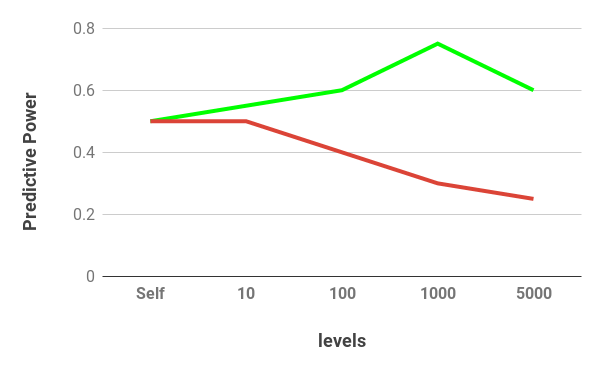
\includegraphics[width=\linewidth]{figs/predictive_power.png}
    \caption{Two hypothetical results about how training set size might effect the efficacy of quality prediction for software projects.}
    \label{fig:predictive_power}
\end{figure}

Petersen and Wohlin~\cite{Petersen2009} argue that for empirical SE, context matters.That is, they would predict that one model  will NOT  cover all  projects and that tools that report  generality  over many software projects need to also know the {\em communities} within which those conclusions   apply. Hence, this work divides into (a)~automated methods for finding sets of projects in the same {\em community}; and (b)~within each {\em community}, find the model what works best. 

The {\em size} of the communities found in this way would have a profound impact on how we should reason about software engineering. Consider the hypothetical results of Figure~\ref{fig:predictive_power}. The \textcolor{ao(english)}{{\bf GREEN}} curve shows some quality predictor that (hypothetically) gets better, the more projects it learns from (i.e. higher levels in the hierarchical cluster). After about 2 levels, the \textcolor{ao(english)}{{\bf GREEN}} curve's growth stops and we would say that community size here was around cluster size in level 1. In this case, while we could not offer a single model that cover {\em all} of SE, we could offer a handful of models, each of which would be relevant to project clusters in that level. Accordingly, we would say that there are many cases where  wisdom from prior projects can be readily applied to guide future projects and (b)~the generality issues raised are not be so pressing.

Now consider the hypothetical \textcolor{red}{{\bf RED}} curve of Figure~\ref{fig:predictive_power}. Here, we see that (hypothetically)  learning from more projects makes quality predictions worse which means the our 10,000 projects break up into ``communities'' of size one. In this case,  (a)~principles about what is ``best practice'' for different software projects would be constantly change (whenever we jump from small community to small community); and (b)~the generality issues would be become open and urgent concerns for the SE analytics community.


\subsection{Related Work}
\label{sec:related}

In this section, we ask ``Why even bother to transfer lessons learned between projects?''. In several recent studies ~\cite{bettenburg2012think, menzies2012local, posnett2011ecological} with readily-available data from SE repositories, numerous authors report the locality effect in SE; i.e. general models outperformed by specialized models localized to particular parts of the data. Menzies et al. showed in their paper about local vs global learning in defect prediction and effort estimation domain that using a rule based learner locality based learning was much effective then rules learned from the global dataset. While Herbold et al.~\cite{herbold2017global} in their study regarding global vs local model for cross-project defect prediction showed evident proof that local models make only a minor difference in comparison to global models. While local can cause conclusion instabilities, global models can miss details which is specific to certain dataset. So in this study, we review the evidence that if it is useful to explore more than just the local data. This evidence falls into four groups:

\textbf{(a) The lesson on big data is that that the {\em more} training data, the {\em better} the learned model.} Vapnik~\cite{vapnik14} discusses examples where models accuracy improves to nearly 100\%, just by training on $10^2$ times as much data. This effect has yet to be seen in SE data~\cite{menzies2013guest} but that might just mean we have yet to use enough training data (hence, this study). 

\textbf{(b) We need to learn from more data since there is very little agreement on what has been learned to far:} Another reason to try generalizing across more SE data is that, among developers, there is little agreement on what many issues relating to software:
\bi
    \item
    According to Passos et al.~\cite{passos11},  developers often  assume that the lessons they learn from a few past projects are general to all their future projects. They comment, ``past experiences were taken into account without much consideration for their context'' ~\cite{passos11}. 
	\item
	J{\o}rgensen \& Gruschke~\cite{Jo09} offer a similar warning. They report that the suppose software engineering ``gurus'' rarely use lessons from past projects to improve their future reasoning and that such poor past advice can be detrimental to new projects.~\cite{Jo09}.
    \item 
    Other studies have shown some widely-held views are   now questionable given new evidence. Devanbu et al. examined responses from 564 Microsoft software developers from around
	the world. They comment programmer beliefs can vary with each project, but do not necessarily
	correspond with actual evidence in that project~\cite{De16}. 
\ei
	
The good news is that, using software analytics, we can correct the above misconceptions. If data mining shows that doing  XYZ is bug prone, then we could  guide developers to avoid XYZ. But will developers listen to us? If they ask ``are we sure  XYZ causes problems?'', can we say that we have mined enough projects to ensure that XYZ is problematic? 

It turns out that developers are not the only ones confused about how various factors influence software projects. Much recent research calls into question  the``established widoms'' of SE field. For example, here is a list of recent conclusions that contradict prior conclusions:

\bi

    \item In stark contrast to  much prior research, pre- and post- release failures are not connected~\cite{fenton2000quantitative};
    
    \item Static code analyzers perform no better than simple statistical predictors~\cite{Fa13}; 
    
    \item The language construct GOTO, as used in contemporary practice, is rarely considered harmful~\cite{nagappan2015empirical};
    
    \item Strongly typed languages are not associated with successful projects~\cite{ray2014large};  
    
    \item Test-driven development is not any better than "test last"~\cite{fucci2017dissection};
    
    \item Delayed issues are not exponentially more expensive to fix~\cite{menzies2017delayed};

\ei

Note that if the reader disputes any of the above, then we ask how would you challenge the items on this list? Where would you get the data, from enough projects, to   successfully refute the above? And where would you get that data? And how would you draw conclusions from that large set?

\textbf{(c) Imported data can be more useful than local data:} Another benefit of  importing data from other projects is that, sometimes, that imported data can be better than the local information. For example, Rees-Jones reports in one study that while building predictors
for Github close time  for open source projects~\cite{rees2017better} using data from other projects performs much better then building models using {\em local learning} (because there is better  information {\em there} than {\em here}).


\textbf{(d) When there is insufficient local data, learning from other projects is very useful:} When developing new software in  novel areas, it is useful to draw on the relevant  experience  from related areas with a larger experience base.This is particularly true when developers are doing something that is novel to them, but has been widely applied elsewhere
For example, Clark and Madachy~\cite{clark15} discuss 65 types of software they see        under-development by the US Defense Department in 2015.   Some of these types are very common (e.g. 22 ground-based communication systems) but other types are very rare (e.g. only  one avionics communication system). (e.g. workers on   flight avionics   might check for lessons learned from ground-based communications). Developers  working in an uncommon area (e.g. avionics communications) might want to transfer in lessons from more common areas (e.g. ground-based communication).


This fuels the art of moving data and/or lessons learned from one project or another is Transfer Learning. This is when there is insufficient data to apply data miners to learn defect predictors, transfer learning can be used to transfer lessons learned from other source projects S to the target project T .

Initial experiments with transfer learning offered very pessimistic results. Zimmermann et al.~\cite{zimmermann2009cross} tried to port models between two web browsers (Internet Explorer and Firefox) and found that cross-project prediction was still not consistent: a model built on Firefox was useful for Explorer, but not vice versa, even though both of them are similar applications. Turhan's initial experimental results were also very negative: given data from 10 projects, training on S = 9 source projects and testing on T = 1 target projects resulted in alarmingly high false positive rates (60\% or more). Subsequent research realized that data had to be carefully sub-sampled and possibly transformed before quality predictors from one source are applied to a target project. Transfer learning can be have two variants - 

\bi
    \item \textbf{Homogeneous Transfer Learning:} This kind of transfer learning operates on source and target data that contain the same attributes.
    
    \item \textbf{Heterogeneous Transfer Learning:} This type of transfer learning operates on source and target data that contain the different attributes.
\ei

Another way of to divide transfer learning is the approach that is followed. There are  2 approaches that is frequently used in many research  - 

\bi
    \item \textbf{Similarity Based Approach:} In this approach we can transfer some/all subset of the rows or columns of data from source to target. For example, the Burak filter~\cite{turhan09} builds its training sets by finding the k = 10 nearest code modules in S for every $ t \in T $. However, the Burak filter suffered from the all too common instability problem (here, whenever the source or target is updated, data miners will learn a new model since different code modules will satisfy the k = 10 nearest neighbor criteria). Other researchers ~\cite{kocaguneli2012, kocaguneli2011find} doubted that a fixed value of k was appropriate for all data. That work recursively bi-clustered the source data, then pruned the cluster sub-trees with greatest ``varianc'' (where the ``variance'' of a sub-tree is the variance of the conclusions in its leaves). This method combined row selection with row pruning (of nearby rows with large variance). Other similarity methods~\cite{Zhang16aa} combine domain knowledge with automatic processing: e.g. data is partitioned using engineering judgment before automatic tools cluster the data. To address variations of software metrics between different projects, the original metric values were discretized by rank transformation according to similar degree of context factors.
    
    \item \textbf{Dimensionality Transformation Based Approach:} In this approach we manipulate the raw source data until it matches the target. An initial attempt on performing transfer learning with Dimensionality transform was undertaken by Ma et al.~\cite{Ma2012} with an algorithm called transfer naive Bayes (TNB). This algorithm used information from all of the suitable attributes in the training data. Based on the estimated distribution of the target data, this method transferred the source information to weight instances the training data. The defect prediction model was constructed using these weighted training data. Nam et al.~\cite{Nam13} originally proposed a transform-based method that used TCA based dimensionality rotation, expansion, and contraction to align the source dimensions to the target. They also proposed a new approach called TCA+, which selected suitable normalization options for TCA, When there are no overlapping attributes (in heterogeneous transfer learning) Nam et al.~\cite{Nam2015} found they could dispense with the optimizer in TCA+ by combining feature selection on the source/target following by a Kolmogorov-Smirnov test to find associated subsets of columns. Other researchers take a similar approach, they prefer instead a canonical-correlation analysis (CCA) to find the relationships between variables in the source and target data~\cite{jing2015heterogeneous}.
\ei

Considering all the attempts at transfer learning sampled above, suggested a surprising lack of consistency in the choice of datasets, learning methods, and statistical measures while reporting results of transfer learning. This issue was addressed by ``Bellwether'' suggested by Krishna et al. ~\cite{krishna2017simpler,krishna16}. which is a simple transfer learning technique is defined in 2- folds namely the Bellwether effect and the Bellwether method:

\bi

    \item \textbf{The Bellwether effect} states that, when a community works on multiple software projects,  then there exists one exemplary project, called the bellwether, which can define predictors for the others.
    
    \item \textbf{The Bellwether method} is where we search for the exemplar bellwether project and construct a transfer learner with it. This transfer learner is then used to predict for effects in future data for that community.

\ei

In their paper Krishna et al. performs experiment with communities of 3, 5 and 10 projects in each, and shows that bellwethers are not rare, their prediction performance is better than local learning, they do fairly well when compared with State of the Art transfer learning methods discussed above and with selection of bellwether shows a consistency for choice of source dataset for transfer learning. This motivated us to use ``Bellwether'' as our choice of method for transfer learning to search for generality in SE datasets. But as per Krishna et al. in order to find bellwether we need to do a $ N*(N-1) $ comparison which is order of $ N^2 $ (N being the number of projects in community). This indeed a very expensive computation. This motivated our study to find generality in SE datasets using a faster Bellwether method. 

Include details about BIRCH and effect of clustering and talk about divide and conquer. 

\section{Data Collection}
\label{sec:Data Collection}

\subsection{Data}
\label{sec:data}

To perform our experiments we choose to work with defect prediction datasets. We use data collected by zhang et al.~\cite{zhang15}. The original data was initially collected by Mockus et al.~\cite{mockus2009amassing} from SourceForge and GoogleCode and was updated till 2010. The dataset contains the full history of about 154K projects that are hosted on SourceForge and 81K projects that are hosted on GoogleCode to the date they were collected. In the original dataset each file contained the revision history and commit logs linked using a unique identified. Although there were 235K projects in the original database, we know from previous literature surveys and experience there were many trivial and non-software development projects. zhang et al. cleaned the dataset using 5 different criteria which resulted in 1385 projects being selected in the final datasets. As part of this experiment we also included few filters to select a subset of 1385 projects, which are useful for our experiment. This eventually gave us a dataset of 697 projects. The filters applied to filter out trivial projects are - 

\bi

    \item \textbf{Programming Languages:} Filtering Out Projects by Programming Languages(only object-oriented i.e *.c, *.cpp, *.cxx, *.cc, *.cs, *.java, and *.pas). This was done as the dataset was collected using a commercial tool, called Understand~\cite{visualize}(which supports the object oriented programming languages) , to compute code metrics. 

    \item \textbf{Projects with a Small Number of Commits:} As small number of commits can mean the projects do not follow a proper SE development process or they are very new, also small number of commits can not provide enough information for computing process metrics and mining defect data. Thus zhang et al. removed any projects with less than 32 commits(25 \% quantile of the number of commits as the threshold).
    
    \item \textbf{Projects with Lifespan Less Than One Year:} zhang et al. collected data in the six-months period using a split date from the first commit and compute process metrics using the change history in the six-months period before the split date. For this reason projects with a lifespan less than one year were filtered out.
    
    \item \textbf{Projects with Limited Defect Data:} For this study defect data was mined using commit messages and bug tracking reports. zhang et al. in their study counted the number of fix-inducing and non-fixing commits from a one-year period and used 152 and 1,689 commits for fix-inducing and non-fixing  respectively for SourceForge. Similarly  92 and 985 commits for GoogleCode. This number was decided by calculating the 75 \% quantile of the number of fix-inducing and non-fixing commits.
    
    \item \textbf{Projects Without Fix-Inducing Commits:} zhang et al. filtered out projects that have no fix-inducing commits during six months as abnormal projects, as projects in defect prediction studies need to contain both defective and non-defective commits.
    
    \item \textbf{Projects with less than 50 rows:} We removed any project with less than 50 rows as they are too small to build a meaningful predictor. 

\ei

\begin{figure}
    \centering
    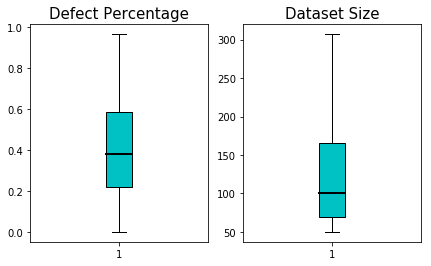
\includegraphics[width=\linewidth]{figs/meta.png}
    \caption{Two hypothetical results about how training set size might effect the efficacy of quality prediction for software projects.}
    \label{fig:meta}
\end{figure}


Along with above filtering criteria, there were few projects which didn't have enough fix-inducing vs non-fixing data points to to create a stratified k=5 fold cross-validation and we removed those projects from the final datasets. These criteria culled 99\% of projects by zhang et al. and culled 54\% of the remaining by our criteria, thus resulted in 697 projects in the final dataset.

From these selected projects, the data was labeled using issue tracking system and commit messages. If a project used issue tracking system for maintaining issue/defect history the data was labeled using that. But as per zhang et al. 42\% of the projects didn't not used issue tracking systems. For these projects labels were created analyzing commit messages by tagging them as fix-inducing commit if commit message matches the following regular expression - 

\begin{center}
\textit{(bug |fix |error |issue |crash |problem |fail |defect |patch)}
\end{center}
 

\subsection{Metric Extraction}
\label{sec:Metric Extraction}

For building any defect predictor we rely on software metrics. Software metrics can be categorized into 3 types according to Xenos \cite{Xenos} distinguishes software metrics as  follows (a) {\em Product metrics} are metrics that are directly related to the product itself, such as code statements, delivered executable, manuals, and strive to measure product quality, or attributes of the product that can be related to product quality. (b) {\em Process metrics} focus on the process of software development and measure process characteristics, aiming to detect problems or to push forward successful practices. Lastly, (c) {\em personnel metrics} (a.k.a. {\em resource metrics}) are those related to the resources required for software development and their performance. The capability, experience of each programmer and communication among all the programmers are related to product quality \cite{wolf2009predicting,de2004sometimes,cataldo2013coordination,cataldo2007coordination}. zhang et al. selected and calculated 21 product and 5 process metrics to build their universal defect prediction model, we will be using the same set of metrics for our study. The product metrics are computed by the Understand tool~\cite{visualize} using the files from the snapshot on the split date of 6 months. The process metrics are computed using the change history in the six-months period before the split date my manual collection of data using scripts. The metrics used in this study are described in table~\ref{tbl:metric}.

\small{
\begin{table}[]
\caption{List of software metrics used in this study}
\label{tbl:metric}
\scriptsize
\begin{tabular}{|p{1cm}|c|l|p{3cm}|}
\hline
\multicolumn{1}{|l|}{Metric}        & \multicolumn{1}{l|}{Metric level} & Metric Name & Metric Description             \\ \hline
\multirow{21}{*}{Product   } & \multirow{6}{*}{File}             & LOC         & Lines of Code                  \\ \cline{3-4} 
                                  &                                   & CL          & Comment Lines                  \\ \cline{3-4} 
                                  &                                   & NSTMT       & Number of Statements           \\ \cline{3-4} 
                                  &                                   & NFUNC       & Number of Functions            \\ \cline{3-4} 
                                  &                                   & RCC         & Ratio Comments to Code         \\ \cline{3-4} 
                                  &                                   & MNL         & Max Nesting Level              \\ \cline{2-4} 
                                  & \multirow{12}{*}{Class}           & WMC         & Weighted Methods per Class     \\ \cline{3-4} 
                                  &                                   & DIT         & Depth of Inheritance Tree      \\ \cline{3-4} 
                                  &                                   & RFC         & Response For a Class           \\ \cline{3-4} 
                                  &                                   & NOC         & Number of Immediate Subclasses \\ \cline{3-4} 
                                  &                                   & CBO         & Coupling Between Objects       \\ \cline{3-4} 
                                  &                                   & LCOM        & Lack of Cohesion in Methods    \\ \cline{3-4} 
                                  &                                   & NIV         & Number of instance variables   \\ \cline{3-4} 
                                  &                                   & NIM         & Number of instance methods     \\ \cline{3-4} 
                                  &                                   & NOM         & Number of Methods              \\ \cline{3-4} 
                                  &                                   & NPBM        & Number of Public Methods       \\ \cline{3-4} 
                                  &                                   & NPM         & Number of Protected Methods    \\ \cline{3-4} 
                                  &                                   & NPRM        & Number of Private Methods      \\ \cline{2-4} 
                                  & \multirow{3}{*}{Methods}          & CC          & McCabe Cyclomatic Complexity   \\ \cline{3-4} 
                                  &                                   & FANIN       & Number of Input Data           \\ \cline{3-4} 
                                  &                                   & FANOUT      & Number of Output Data          \\ \hline
\multirow{5}{*}{Process }  & \multirow{5}{*}{File}             & NREV        & Number of revisions            \\ \cline{3-4} 
                                  &                                   & NFIX        & Number of revisions a file     \\ \cline{3-4} 
                                  &                                   & ADDED LOC    & Lines added                    \\ \cline{3-4} 
                                  &                                   & DELETED LOC  & Lines deleted                  \\ \cline{3-4} 
                                  &                                   & MODIFIED LOC & Lines modified                 \\ \hline
\end{tabular}
\end{table}
}


\section{Experimental Setup}
\label{sec:Experimental}

In this study we try to establish the presence of generality in SE datasets. We do this by analyzing the presence of bellwether incrementally by adding more and more projects and how the bellwether's predictive power changes. In this case to show the presence of generality in SE datasets the predictive power of the bellwether should look like the \textcolor{ao(english)}{GREEN} in figure~\ref{fig:predictive_power}, that is the predictive power of bellwether should increase or remains same, if our results look like the \textcolor{red}{RED} curve, that will show absence of generality in SE datasets.

In order to achieve this we try to explore the \textit{bellwether effect} as mentioned in ~\ref{sec:related}. We know the default \textit{bellwether method} is very expensive ($ O(N^2) $). Thus in this paper we proposes an alternative transfer learning method (BUBBLE), that explores \textit{bellwether effect} by exploring an order of magnitude faster \textit{bellwether method}. Our approach has three key components:

\bi

    \item A feature extractor to find a representation of each project, which will be used for clustering the projects. 
    
    \item A hierarchical clustering model to use the features extracted from previous step to build the hierarchical cluster.
    
    \item A transfer learning model to identify bellwether in the hierarchical cluster.

\ei

BUBBLE employs few different algorithms to complete and compose it's 4 different components - 

\subsection{Feature Subset Selection (FSS)}
\label{subsec:FSS}
To extract features from each dataset, we use a feature selector algorithm called Feature Subset Selection(FSS)~\cite{hall1999correlation,hall1997feature}. Which is a process of identifying and removing as much irrelevant and redundant information as possible. This is achieved using a correlation based feature evolution strategy to evaluate importance of an attribute and a best first search strategy with back tracking that moves through the search space by making local changes to the current feature subset.Here if the path being explored begins to look less promising, the best first search can back-track to a more promising previous subset and continue the search from there. Given enough time, a best first search will explore the entire search space, so it uses a stopping criterion (i.e. no improvement for five consecutive attributes). XXX

\small{
\begin{figure}[]
    \small
     \begin{lstlisting}[mathescape,linewidth=7.5cm,frame=none,numbers=right]
      def CFS(data):
        features = []
        score = -0.000000001
        while True:
            best_feature = None
            for feature in range(data.features):
                features.append(feature)
                temp_score = calculate_corr(data[F])
                if temp_score > score:
                    score = temp_score
                    best_feature = features
                features.pop()
            features.append(best_feature)
            if not improve(score):
                break
        return features
    
    \end{lstlisting} 
    \vspace{-0.2cm}
    \caption{Pseudo-code of Feature Subset Selection}
    \label{fig:GAP_pseudocode} 
    \vspace{-0.3cm}
\end{figure}
}
\subsection{Balanced Iterative Reducing and Clustering using Hierarchies (BIRCH)}
\label{subsec:BIRCH}
To find presence or absence of generality in SE datasets, we need to incrementally check for ``Bellwether'' from smaller to larger community. A community is a set of project which is similar in nature. We use the BIRCH algorithm on our defect prediction dataset to create a hierarchical clustering tree to form these communities. BIRCH~\cite{zhang1996birch} is  a hierarchical clustering algorithm, which has a ability to incrementally and dynamically cluster incoming, multi-dimensional data in an attempt to produce the best quality clustering. BIRCH also has the ability to identify data points that are not part of the underlying pattern effectively identifying outliers. In this study we uses a modified BIRCH algorithm to store additional information regarding each cluster in the clustering feature tree, which help us in the experiment. XXX

\subsection{Synthetic Minority Over-Sampling Technique (SMOTE)}
\label{subsec:SMOTE}

Machine learning models exploits the inherent bias in the dataset to segregate and classify different classes. Hence class imbalance can create major bias towards the majority class when building a machine learning model, thus producing biased model which provides bad classification results. Synthetic Minority Over-Sampling Technique (SMOTE)~\cite{chawla2002smote} is a technique to handle class imbalance by changing the frequency of different classes of the training data. When applied to data, SMOTE sub-samples the majority class (i.e., deletes some examples) while over-sampling the minority class until all classes have the same frequency. In the case of software defect data, the minority class is usually the defective class. During super-sampling, a member of the minority class finds k nearest neighbors. It builds an artificial member of the minority class at some point in-between itself and one of its random nearest neighbors. During that process, some distance function is required which is the \textit{minkowski distance} function.

\subsection{Logistic Regression (LR)}
\label{subsec:LR}

Logistic regression is a statistical machine learning model that in its basic form uses a logistic function to model a binary dependent variable. In this study we use scikit learn's default logistic regression implementation as our learner for building source models and evaluating on target models inside each community. In this study we selected logistic regression, as it is very fast to build in comparison to other more complex learners and its much more comprehensible and explainable in-terms of attributes and their importance. Logistic Regression is widely used in defect prediction domain and have shown promising results both in-term of predictive power and comprehensibility.


\subsection{Bellwether\_0:}
\label{Bellwether}

In this study to compare our novel method to the state of the art method, we uses Krishna et al. 's \textit{bellwether method}. We use all the projects available in the community to perform a $N*(N-1)$ comparison, where N is the number of projects in the community to measure the performance of each project measured on all others on the performance measures mentioned in sec~\ref{sec:Measures}. Following this we use cdom function to select a bellwether project among them. 



\subsection{BUBBLE}
\label{BUBBLE}

BUBBLE is a \textit{bellwether method} algorithm which combines the components described above, to create a fast way to find \textit{bellwether effect}. BUBBLE works in 6 stages - 

    (1) \textbf{Feature Extraction:} In this stage the whole dataset is used to extract feature from each projects. This is done using the FSS algorithm as shown in~\ref{subsec:FSS}. Here each project is sent to the FSS and the FSS returns most suitable features for building models, we do this for every project and that information as a vector (i.e. a vector or length equal to total number of features, where 1 represents a feature being selected ,0 is the other way around) that represents each project. By performing this we have a vector representation of each project in the dataset. BUBBLE uses this information to create the hierarchical clusters to find the communities. We perceive this is a good representation of community, as in this work we try to find community which has similar information distribution according to the attributes. Thus 2 projects with similar features selected have much higher chance of building similar models.
    
    (2) \textbf{Cluster Creation:} After the feature extraction has been done, the data is sent to a modified BIRCH algorithm. The algorithm requires a branching factor (i.e. Maximum number of CF sub-clusters in each node) and threshold value (i.e. when to form a new cluster based on radius). For this experiment we have set the branching factor as 20 and threshold value as 0.5. Using this version of BIRCH algorithm we build the hierarchical cluster, while storing all necessary details about the cluster like parent-child node, data points, level information etc. This stage returns a Clustering Feature Tree (CF Tree) with all those information, which is passed to the next phase of experiment. 
    
    (3) \textbf{Bellwether selection phase 1:} The CF Tree from the last phase is passed to the hierarchical bellwether. In this phase we use \textit{bellwether method} to identify bellwether at the leaf level. Using the CF Tree, we identify the clusters at the leaf level where each cluster represents the smallest community produced by the BIRCH algorithm in the last phase. Here we use the default ``Bellwether'' to perform a $ N*(N-1) $ comparison at each cluster.Here we select each project in the cluster one by one as a source dataset for transfer learning apply SMOTE as mentioned in sec~\ref{subsec:SMOTE} to handle any data imbalance and then use the FSS algorithm to get rid of any unnecessary attributes as mentioned in sec~\ref{subsec:FSS}. This informative and balanced dataset is used to build a LR model as mentioned in sec~\ref{subsec:LR} and we measure the performance of all other projects in the community(cluster). The performance measures that are used are mentioned in sec~\ref{sec:Measures}. To find the bellwether in each community we use cdom function to find the best source dataset among each cluster considering all performance measures. This phase returns a bellwether for each cluster at the leaf level of the CF Tree.
    
    (4) \textbf{Bellwether promotion:} In this phase of the algorithm is an iterative process, here we receive the selected bellwethers from the child clusters of each cluster in the level. This is called the bellwether promotion. Here each parent cluster instead of being represented by all projects within them, they are represented by only the bellwethers in them.  
    
    (5) \textbf{Bellwether selection phase 2:} In this phase instead of finding a bellwether for each cluster at the level by performing a $ N*(N-1) $ comparison, we select the projects which represented as bellwether at the child nodes and then try to find a bellwether among them. So at each cluster at the level we perform a a $ M*(M-1) $ comparison at each cluster where M is the selected bellwether from child clusters. This creates a order of magnitude faster \textbf{bellwether method}. This is again an iterative process, and the end of all the iterations, we will have a bellwether at each cluster at every level. 
    
    (6) \textbf{Bellwether Prediction:} This is the transfer learning phase, when a new project is to evaluated we will use the FSS algorithm to get its features, then use the feature vectors to identify which cluster it belongs and use that cluster's bellwether as the transfer learning model.


To report the finding and results of this study without any bias, we repeat the experiment 20 times by dividing the dataset randomly into train\_1 and test\_1 as a 90-10 split, the projects in train\_1 was used to find the bellwether in each cluster in the CF Tree, and then each project in test\_1 was divide into train\_2 and test\_2 split. We trained a LR model using train\_2 for each project and tested on test\_2, this is represented as self test in this study. We also used the predict stage of the BUBBLE to identify bellwether for each project in test\_1 and tested the performance on test\_2. 


\small{
\begin{figure}[]
    \small
     \begin{lstlisting}[mathescape,linewidth=7.5cm,frame=none,numbers=right]
      def BUBBLE(data):
        project_features = get_features(data)
        cluster_tree = BIRCH(project_features)
        bellwethers = h_bellwether(cluster_tree)
        for project in test_1:
            train_2,test_2 = train_test_split(data[project])
            self_clf = LR(train_2)
            b_clf = find_bellwether(project_features[project])
            self_score = self_clf.predict(test_2)
            bellwether_score = b_clf.predict(test_2)
            results.append([self_score,bellwether_score]) 
        return results
    \end{lstlisting} 
    \vspace{-0.2cm}
    \caption{Pseudo-code of BUBBLE Experiment}
    \label{fig:GAP_pseudocode} 
    \vspace{-0.3cm}
\end{figure}
}

\small{
\begin{figure}[]
    \small
     \begin{lstlisting}[mathescape,linewidth=7.5cm,frame=none,numbers=right]
      def h_bellwether(cluster_tree):
        bellwethers = { }
        def bellwether(list1,list2):
            for source in list1:
                clf = LR(source)
                _list2 = list2.pop(source)
                for dest in _list2:
                    score[source][dest] = clf.predict(dest)
            return best(score.key())
        for level in cluster_tree.levels:
            if level == cluster_tree.max_level:
                for c in cluster_tree[level].clusters:
                    bellwethers[c] = bellwether(c.projects,
                                                c.projects)
            else:
                for c in cluster_tree[level].clusters:
                    child_clusters = c.child
                    _bellwethers = bellwethers[child_clusters]
                    bellwethers[c] = bellwether(_bellwethers,
                                                _bellwethers)
        return bellwethers
    \end{lstlisting} 
    \vspace{-0.2cm}
    \caption{Pseudo-code of Hierarchical Bellwether}
    \label{fig:GAP_pseudocode} 
    \vspace{-0.3cm}
\end{figure}
}

\subsection{Statistical Tests}
\label{stats}

When comparing the results different models in this study, we used a statistical significance test and an effect size test. Significance test are useful for detecting if two populations
differ merely by random noise. Also, effect sizes are useful for checking that two populations differ by more than just a trivial amount. For the significance test,  we use the Scott-Knott procedure  recommended at TSE'13~\cite{mittas2013ranking} and ICSE'15~\cite{ghotra2015revisiting}. This technique recursively bi-clusters a sorted set of numbers. If any two clusters are statistically indistinguishable, Scott-Knott reports them both as one group. Scott-Knott first looks for a break in the sequence that maximizes the expected values in the difference in the means before and after the break.More specifically,  it  splits $l$ values into sub-lists $m$ and $n$ in order to maximize the expected value of differences  in the observed performances before and after divisions. For e.g., lists $l,m$ and $n$ of size $ls,ms$ and $ns$ where $l=m\cup n$, Scott-Knott divides the sequence at the break that maximizes:

\begin{equation}
    E(\Delta)=ms/ls*abs(m.\mu - l.\mu)^2 + ns/ls*abs(n.\mu - l.\mu)^2\
\end{equation}

Scott-Knott then applies some statistical hypothesis test $H$ to check if $m$ and $n$ are significantly different. If so, Scott-Knott then recurses on each division. For this study, our hypothesis test $H$ was a conjunction of the A12 effect size test (endorsed by \cite{arcuri2011practical})  and non-parametric bootstrap sampling \cite{efron94}, i.e., our Scott-Knott divided the data if {\em both} bootstrapping and an effect size test agreed that the division was statistically significant (90\% confidence) and not a ``small'' effect ($A12 \ge 0.6$).

\subsection{Continuous Domination(cdom)}
\label{cdom}
In this study, we compare each project's performance against all other projects in each cluster at the leaf level of the BIRCH as described in section~\ref{BUBBLE} and section~\ref{Bellwether}. We calculate 5 different performance measure for each project as described in section~\ref{sec:Measures}. In order to find a \textit{bellwether effect} in the performances collected we need to combine those 5 performance measures and then rank them using certain criteria. We have used continuous domination (cdom) for this purpose. continuous domination is defined as the set of all points in the objective space that are not dominated by any other points. Unlike Boolean domination, which says a point is dominated by another if and only if the first point is better in every single objective then the second point, continuous domination combines all the objective into a continuous function to compare and then calculate if one point dominates another. Throughout literature continuous domination has proven to be very effective when multiple goals are concerned. The continuous domination function is defined as below, where P is the total population, k is fitness scaling factor and $X\_1$ is the data points we are calculating the domnation for - 

\begin{equation}
    F(X_1) = \sum_{{(X_2\in P) - X_1}} -e^{-I(X_2,X_1)/k}
\end{equation}


\section{Performance Measures}
\label{sec:Measures}

In this section, we introduce the following 5 evaluation measures used in this study to evaluate the performance of machine learning models. Suppose we have a dataset with M changes and N defects. After inspecting 20\% LOC, we inspected m changes and found n defects. Besides, when we find the first defective change, we have inspected k changes. Then the 5 evaluation measures are defined and computed as follows:

(1) \textbf{Recall:} Proportion of inspected defective changes among all the actual defective changes. This is the evaluation measure used by many previous studies~\cite{kamei2012large,yang2016effort,yang2017tlel,xia2016collective,yang2015deep} . They focused on achieving high Recall so that more defective changes could be detected. Recall is computed as: $n/N$.

(2) \textbf{Precision:} Proportion of inspected defective changes among all the inspected changes. A low Precision indicates that developers would encounter more false alarms, which may have negative impact on developers' confidence on the prediction model. Precision is computed as: $n/m$.

(3) \textbf{pf:} Proportion of all suggested defective changes which are not actual defective changes among all the suggested defective changes. A high pf suggests developers will encounter more false alarms which may have negative impact on developers' confidence on the prediction model.

(4) \textbf{popt20:} Proportion number of suggested defective changes among all suggested defective changes, when when 20\% LOC modified by all changes are inspected. A high popt20 indicates that, under the same number of LOC to inspect, developers developers will find more bugs, which means developers will be able to fix more defects with same amount of effort invested. XXX

(5) \textbf{ifa:} Number of Initial False Alarms encountered before we find the first defect. Inspired by previous studies on fault localization~\cite{parnin2011automated,kochhar2016practitioners,xia2016automated}, we assume that if the top-k changes recommended by the model are all false alarms, developers would be frustrated and are not likely to continue inspecting the other changes. For example, Parnin and Orso ~\cite{parnin2011automated} investigated how developers use and benefit from automated debugging tools through a set of human studies. They found that developers would stop inspecting suspicious statements, and turn back to traditional debugging, if they could not get promising results within the first few statements they inspect. ifs is computed as: k.


\section{Results}
\label{sec:results}

\subsection{RQ1: Can we confirm bellwether on large datasets?}
\label{sec:rq1}

In the literature, we saw most of the previous studies has shown bellwether effect with very small datasets. In order to use bellwether to prove presence of generality in SE domain datasets, we first have to showcase the bellwether method suggested by Krishna et al. in their experiment works for large datasets. We use our defect prediction dataset with 697 projects for this purpose. We divide the dataset in train\_1 and test\_1 set and then performed a $ N*(N-1) $ comparison on all the projects in train\_1 set to find a bellwether, and then dividing each project in test\_1 set into train\_2 and test\_2 using a train\_test split. We use the train\_2 to train a LR model and test on test\_2 which is represented as \textit{self\_0} in the figures. Similarly we use the bellwether project from train\_1 to train a LR model and test it on test\_2 which is represented as \textit{bellwether0}. We use statistical tests mentioned in section~\ref{stats} to compare the performance of \textit{self\_0} vs \textit{bellwether0} for all the performance measures mentioned in section~\ref{sec:Measures}, which is shown in figure~\ref{fig:recall}, \ref{fig:precision}, \ref{fig:pf}, \ref{fig:popt20}, \ref{fig:ifa} . It is evident that using the \textit{bellwether method} proposed by Krishna et al. we were able to find bellwether effect in large dataset with 697 projects. This answers this RQ and creates the baseline results for our study. In this RQ1 although we are able to find \textit{bellwether effect}, this method is very expensive, requiring a $ N*(N-1) $ comparison, which in our experimental setup took nearly 75 days of computation on a single core machine. Which takes us to the next research question. 



\subsection{RQ2: How to tame complexity of bellwether?}
\label{sec:rq2}

To tame complexity of bellwether in this RQ, we propose a new bellwether method called ``BUBBLE'' to find bellwether in large datasets. This bellwether method is composed of 6 stages, (a) a feature extraction process to summarize each project into a single representative vector, (b) a hierarchical clustering algorithm, which uses the feature vectors to cluster similar projects into community of increasing size at different levels of cluster, (c) a bellwether selection phase where a $N*(N-1)$ comparison is performed at each leaf level cluster and using a cdom calculation in all the metrics mentioned in~\ref{tbl:metric} a bellwether is selected, (d) a iterative bellwether promotion stage, where bellwether from child clusters are promoted as potential bellwethers at parent cluster, (e) another bellwether selection phase at non-leaf levels, where comparisons are only made among potential bellwethers from leaf node and finally (f) a bellwether prediction phase, which suggests a bellwether based on project similarity when a new project is to be predicted. The details of each phase is mentioned in sec~\ref{BUBBLE}. 

In the \textit{bellwether method} proposed by Krishna et al. if there are N projects in a community it will make $\approx N^2$ comparisons to discover the bellwether. While ``BUBBLE'' different approach to discover bellwether by dividing the data into smaller cluster and finding bellwether among each, here if we assume we have m cluster at leaf level with N projects in each, we will have 
$\approx N^2/m$ comparisons to discover the bellwether which is m times less comparison. Using this process we able to find bellwether in ~1.5 hours, which is order of magnitude faster then the bellwether method proposed by Krishna et al. 

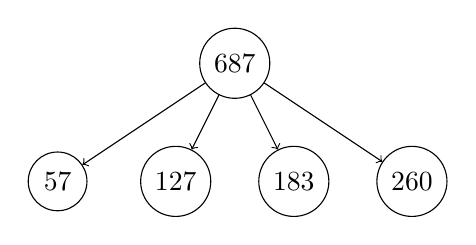
\begin{tikzpicture}[nodes={draw, circle}, ->]
 
    \node{687}
        child { node {57} }
        child { node {127} }
        child { node {183} }
        child { node {260} };
 
\end{tikzpicture}



%%%%%%%%%%%%%%%%%%%%%%%%%%%%%%%%%%%%%%%%%%%%%%%%%%%%%%%%%%%
%%%%%%%%%%%%%%%%%%%%%%%Latex Table%%%%%%%%%%%%%%%%%%%%%%%%%
\begin{figure}[!t]
{\small
{\small \begin{tabular}{llrrc}
\arrayrulecolor{darkgray}
\rowcolor[gray]{.9}  rank & treatment & median & IQR & \\
    1 &      self\_0 &    50 &  86 & \quart{0}{50}{86}{36} \\
    2 &      bellwether0 &    67 &  64 & \quart{36}{67}{64}{33} \\
    2 &      bellwether\_level2 &    67 &  67 & \quart{33}{67}{67}{33} \\
    2 &      bellwether\_level1 &    67 &  62 & \quart{38}{67}{62}{33} \\
    3 &      bellwether\_level0 &    78 &  50 & \quart{50}{78}{50}{22} \\
\end{tabular}}
}
\caption{Recall
}\label{fig:recall}
\end{figure}
%%%%%%%%%%%%%%%%%%%%%%%End Latex Table%%%%%%%%%%%%%%%%%%%%%
%%%%%%%%%%%%%%%%%%%%%%%%%%%%%%%%%%%%%%%%%%%%%%%%%%%%%%%%%%%

%%%%%%%%%%%%%%%%%%%%%%%%%%%%%%%%%%%%%%%%%%%%%%%%%%%%%%%%%%%
%%%%%%%%%%%%%%%%%%%%%%%Latex Table%%%%%%%%%%%%%%%%%%%%%%%%%
\begin{figure}[!t]
{\small
{\small \begin{tabular}{llrrc}
\arrayrulecolor{darkgray}
\rowcolor[gray]{.9}  rank & treatment & median & IQR & \\
    1 &      bellwether\_level0 &    43 &  47 & \quart{20}{43}{47}{24} \\
    1 &      bellwether0 &    44 &  47 & \quart{20}{44}{47}{23} \\
    1 &      bellwether\_level2 &    50 &  51 & \quart{20}{50}{51}{21} \\
    1 &      bellwether\_level1 &    50 &  51 & \quart{20}{50}{51}{21} \\
    1 &      self\_0 &    60 &  83 & \quart{0}{60}{83}{23} \\
\end{tabular}}
}
\caption{Precision
}\label{fig:precision}
\end{figure}
%%%%%%%%%%%%%%%%%%%%%%%End Latex Table%%%%%%%%%%%%%%%%%%%%%
%%%%%%%%%%%%%%%%%%%%%%%%%%%%%%%%%%%%%%%%%%%%%%%%%%%%%%%%%%%

%%%%%%%%%%%%%%%%%%%%%%%%%%%%%%%%%%%%%%%%%%%%%%%%%%%%%%%%%%%
%%%%%%%%%%%%%%%%%%%%%%%Latex Table%%%%%%%%%%%%%%%%%%%%%%%%%
\begin{figure}[!t]
{\small
{\small \begin{tabular}{llrrc}
\arrayrulecolor{darkgray}
\rowcolor[gray]{.9}  rank & treatment & median & IQR & \\
    1 &      self\_0 &    20 &  50 & \quart{0}{20}{50}{30} \\
    2 &      bellwether0 &    50 &  55 & \quart{25}{50}{55}{30} \\
    2 &      bellwether\_level2 &    50 &  54 & \quart{21}{50}{54}{25} \\
    2 &      bellwether\_level1 &    50 &  50 & \quart{25}{50}{50}{25} \\
    3 &      bellwether\_level0 &    67 &  67 & \quart{33}{67}{67}{33} \\
\end{tabular}}
}
\caption{PF
}\label{fig:pf}
\end{figure}
%%%%%%%%%%%%%%%%%%%%%%%End Latex Table%%%%%%%%%%%%%%%%%%%%%
%%%%%%%%%%%%%%%%%%%%%%%%%%%%%%%%%%%%%%%%%%%%%%%%%%%%%%%%%%%

%%%%%%%%%%%%%%%%%%%%%%%%%%%%%%%%%%%%%%%%%%%%%%%%%%%%%%%%%%%
%%%%%%%%%%%%%%%%%%%%%%%Latex Table%%%%%%%%%%%%%%%%%%%%%%%%%
\begin{figure}[!t]
{\small
{\small \begin{tabular}{llrrc}
\arrayrulecolor{darkgray}
\rowcolor[gray]{.9}  rank & treatment & median & IQR & \\
    1 &      bellwether0 &    33 &  21 & \quart{25}{33}{21}{13} \\
    1 &      self\_0 &    33 &  50 & \quart{0}{33}{50}{17} \\
    1 &      bellwether\_level2 &    33 &  20 & \quart{25}{33}{20}{12} \\
    1 &      bellwether\_level0 &    33 &  16 & \quart{27}{33}{16}{10} \\
    1 &      bellwether\_level1 &    33 &  20 & \quart{25}{33}{20}{12} \\
\end{tabular}}
}
\caption{Popt20
}\label{fig:popt20}
\end{figure}
%%%%%%%%%%%%%%%%%%%%%%%End Latex Table%%%%%%%%%%%%%%%%%%%%%
%%%%%%%%%%%%%%%%%%%%%%%%%%%%%%%%%%%%%%%%%%%%%%%%%%%%%%%%%%%


%%%%%%%%%%%%%%%%%%%%%%%%%%%%%%%%%%%%%%%%%%%%%%%%%%%%%%%%%%%
%%%%%%%%%%%%%%%%%%%%%%%Latex Table%%%%%%%%%%%%%%%%%%%%%%%%%
\begin{figure}[!t]
{\small
{\small \begin{tabular}{llrrc}
\arrayrulecolor{darkgray}
\rowcolor[gray]{.9}  rank & treatment & median & IQR & \\
    1 &      bellwether0 &    1 &  4 & \quartx{0}{1}{4}{3} \\
    1 &      self\_0 &    1 &  5 & \quartx{0}{1}{5}{4} \\
    1 &      bellwether\_level2 &    1 &  4 & \quartx{0}{1}{4}{3} \\
    1 &      bellwether\_level0 &    1 &  4 & \quartx{0}{1}{4}{3} \\
    1 &      bellwether\_level1 &    1 &  4 & \quartx{0}{1}{4}{3} \\
\end{tabular}}
}
\caption{IFA
}\label{fig:ifa}
\end{figure}
%%%%%%%%%%%%%%%%%%%%%%%End Latex Table%%%%%%%%%%%%%%%%%%%%%
%%%%%%%%%%%%%%%%%%%%%%%%%%%%%%%%%%%%%%%%%%%%%%%%%%%%%%%%%%%


\subsection{RQ3: Is faster bellwether effective?}
\label{sec:rq3}

In RQ2, we can see using ``BUBBLE'' we are able to find bellwether for a large dataset in order of magnitude faster. This raises the question is  \textit{bellwether method} ``BUBBLE'' as effective as \textit{bellwether method} proposed by krishna et al.? To answer this question in this study we have used the defect prediction dataset with 697 projects and divided the projects randomly into train\_1 and test\_1 as a 90-10 split, the projects in train\_1 was used to find the bellwether in each cluster in the CF Tree as mentioned in sec~\ref{BUBBLE}, and then each project in test\_1 was divide into train\_2 and test\_2 split. We trained a LR model using train\_2 for each project and tested on test\_2 (represented as self\_0), this is represented as self test in this study. We also used the predict stage of the ``BUBBLE'' to identify a bellwether in each level of hierarchical model, for each project in test\_1 and tested the performance on test\_2 (represented as bellwether\_level0, bellwether\_level1, bellwether\_level respectively). Similarly we used the projects in train\_1 to find the bellwether using default bellwether method as mentioned in sec~\ref{Bellwether}, and use that project to build a LR model and test the performance of each project's test\_2 (represented as bellwether0). We compare the performance of each model described above using statistical tests as mentioned in section~\ref{stats} and if 2 models are ranked different that represents their performance is significantly different. We can see from the figure~\ref{fig:recall} that bellwether\_level0 model (i.e. the bellwether discovered by ``BUBBLE'' at level 0) performs best with a median of 78 and IQR of 50. 
We can see from the results in , ~\ref{fig:precision}, ~\ref{fig:pf}, ~\ref{fig:popt20}, ~\ref{fig:ifa}. 


\subsection{RQ4: Should SE uses general methods or cohert based methods?}
\label{sec:rq4}

This RQ is about presence of generality in SE datasets based on the results from ``BUBBLE'' in RQ~\ref{sec:rq1}, RQ~\ref{sec:rq2} and RQ~\ref{sec:rq3}. 

\section{Discussion}
\label{sec:discuss}
What's old is new. Our results 

\section{Threats to Validity}
\label{sec:validity}

As with any large scale empirical study, biases can affect the final
results. Therefore, any conclusions made from this work
must be considered with the following issues in mind:

\bi 

\item \textit{Evaluation Bias}: 
In  RQ1, RQ2 and RQ3 we have shown the performance of local model, hierarchical bellwether models, default bellwether model and compared them using statistical tests on their performance to make conclusion about presence of generality in SE datasets. While those results are true, that conclusion is scoped by the evaluation metrics we used to write this paper. It is possible that, using other measurements, there may well be a difference in these different kinds of projects. This is a matter that needs to be explored in future research.  

    
\item \textit{Construct Validity}: At various places in this report, we made engineering decisions about (e.g.) choice of machine learning models, hierarchical clustering algorithm, selecting feature vectors for each r=project. While those decisions were made using advice from the literature, we acknowledge that other constructs might lead to different conclusions. 

\item \textit{External Validity}: For this study we have relied on data collected by zhang et al.~\cite{zhang15} for their studies. The metrics collected for each project was done using an commercialized tool called ``Understand''. There is a possibility that calculation of metrics or labeling of defective vs non-defective using other tools or methods may result in different outcome. That said, the ``Understand'' is a commercialized tool which has detailed documentation about the metrics calculations and zhang et al. has shared their scripts and process to convert the metrics to usable format and has described the approach to label defects.  

We have relied on issues marked as a `bug' or `enhancement' to count bugs or enhancements, and bug or enhancement resolution times. In Github, a bug or enhancement might not be marked in an issue but in commits. There is also a possibility that the team of that project might be using different tag identifiers for bugs and enhancements. To reduce the impact of this problem, we  did take precautionary step to (e.g.,) include various tag identifiers from Cabot et al.~\cite{cabot2015exploring}. We also took precaution to remove any pull merge requests from the commits to remove any extra contributions added to the hero programmer. 

\item \textit{Statistical Validity}: To increase the validity of our results, we applied two statistical tests, bootstrap and the a12. Hence, anytime in this paper we reported that ``X was different from Y'' then that report was based on both an effect size and a statistical significance test.
 
\item \textit{Sampling Bias}: Our conclusions are based on the 697 projects collected by zhang et al.~\cite{zhang15} for their studies. It is possible that different initial projects would have lead to different conclusions. That said, this sample is very large so we have some confidence that this sample represents an interesting range of projects. As evidence of that, we note that our sampling bias is less pronounced than other ``Bellwether'' studies since we explored.
 
\ei



\section{Conclusion}
\label{sec:concl}

The established wisdom in the literature is to depreciate `

\section{Future Work}
\label{sec:furute}



\section{Acknowledgements}
\label{sec:ack}

The first and second authors conducted this research study as part
of their internship at the industry in Summer, 2017. 


\balance

\bibliographystyle{ACM-Reference-Format}

\bibliography{main}
%
%\documentclass[sigconf]{acmart}
\documentclass[sigconf]{acmart} 
\pdfoutput=1
\usepackage[shortlabels]{enumitem}
\usepackage{balance}
\usepackage{dblfloatfix}

\usepackage{hyperref}
\usepackage{cleveref}
\usepackage{colortbl}
%\usepackage{color}
%\usepackage{booktabs} % For formal tables
%\usepackage{graphicx}
%\usepackage{float}
%\usepackage{listings}
%\usepackage{url}
%\usepackage{comment}
%\usepackage{multirow}
%\usepackage{rotating}
% \usepackage{bigstrut}
% \usepackage{graphics}
% \usepackage{picture}
%\usepackage{cite}

\makeatletter
\let\th@plain\relax
\makeatother


\newcommand{\bi}{\begin{itemize}[leftmargin=0.4cm]}
	\newcommand{\ei}{\end{itemize}}
\newcommand{\be}{\begin{enumerate}[leftmargin=0.4cm]}
	\newcommand{\ee}{\end{enumerate}}


\usepackage{picture}
\newcommand{\quart}[4]{\begin{picture}(100,6)%1
{\color{black}\put(#2,3){\color{red}\circle*{4}}\put(#1,3){\line(1,0){#3}}}\end{picture}}
\newcommand{\quartr}[4]{\begin{picture}(100,6)%1
{\color{black}\put(#2,3){\color{red}\circle*{4}}\put(#1,3){\line(1,0){#3}}}\end{picture}}
\newcommand{\quartx}[4]{\begin{picture}(100,1)%1
{\color{black}\put(\numexpr #2 * 6  \relax,3){\color{red}\circle*{4}}\put(\numexpr #1*6 \relax ,3){\line(1,0){\numexpr #3*6 \relax}}}\end{picture}}

\definecolor{lightgray}{gray}{0.8}
\definecolor{darkgray}{gray}{0.6}
\definecolor{Gray}{gray}{0.85}
\definecolor{Blue}{RGB}{0,29,193}

% \usepackage{tabularx}
% \usepackage{hhline}
% \usepackage[export]{adjustbox}

\definecolor{ao(english)}{rgb}{0.0, 0.5, 0.0}

\definecolor{Gray}{gray}{0.85}
\usepackage{tikz}
\usepackage{framed}
\usepackage[framed]{ntheorem}
\usepackage{multirow}
\usetikzlibrary{shadows}
\usepackage{listings}
\definecolor{MyDarkBlue}{rgb}{0,0.08,0.45} 
\lstset{
    language=Python,
    basicstyle=\sffamily\fontsize{2.5mm}{0.7em}\selectfont,
    breaklines=true,
    prebreak=\raisebox{0ex}[0ex][0ex]{\ensuremath{\hookleftarrow}},
    frame=l,
    keepspaces=false,
    showtabs=false,
    columns=fullflexible,
    showspaces=false,
    showstringspaces=false,
    keywordstyle=\bfseries\sffamily,
    emph={while, for , if ,data, def}, emphstyle=\bfseries\color{blue!50!black},
    stringstyle=\color{green!50!black},
    commentstyle=\color{red!50!black}\it,
    numbers=left,
    captionpos=t,
    escapeinside={\%*}{*)}
}

\theoremclass{Lesson}
\theoremstyle{break}

% inner sep=10pt,
\tikzstyle{thmbox} = [rectangle, rounded corners, draw=black, fill=Gray!40]
\newcommand\thmbox[1]{%
	\noindent\begin{tikzpicture}%
	\node [thmbox] (box){%
		\begin{minipage}{.94\textwidth}%
		\vspace{-0.1cm}#1\vspace{-0.1cm}%
		\end{minipage}%
	};%
	\end{tikzpicture}}

\let\theoremframecommand\thmbox
\newshadedtheorem{lesson}{Result}


% \setcopyright{none}

% % \acmDOI{10.475/123_4}
% % % ISBN
% % \acmISBN{123-4567-24-567/17/08}
% \acmConference[ICSE SEIP'18]{International Conference on Software Engineering, SE in practice track}{May 2018}{Gothenburg, Sweden} 
% \acmYear{2018}
% \copyrightyear{2018}

% \acmPrice{00.00}

%\hyphenation{op-tical net-works semi-conduc-tor}


\begin{document}
%\pagestyle{plain}

\copyrightyear{2018} 
\acmYear{2018} 
\setcopyright{acmcopyright}
\acmConference[ICSE-SEIP '18]{40th International Conference on Software Engineering: Software Engineering in Practice Track}{May 27-June 3, 2018}{Gothenburg, Sweden}
\acmBooktitle{ICSE-SEIP '18: 40th International Conference on Software Engineering: Software Engineering in Practice Track, May 27-June 3, 2018, Gothenburg, Sweden}
\acmPrice{15.00}
\acmDOI{10.1145/3183519.3183549}
\acmISBN{978-1-4503-5659-6/18/05}


\title{BUBBLE}
\subtitle{An Approach to find generality in Software Engineering}

\author{Suvodeep Majumder, Rahul Krishna and Tim Menzies}
\affiliation{Computer Science, NCSU, USA, North Carolina}  
\email{[smajumd3,rkrish11]@ncsu.edu, tim@ieee.org}


\begin{abstract}
Software analytics builds quality prediction models for software projects. After a decade of intensive software analytics there is much disagreement between whether should we use general models that hold over many projects? Or must we use an ever changing set of ideas that are continually adapted to the task at hand? There have many studies that has generated specific results about specific projects~\cite{Bird:2015, menzies2013software} showcasing specificity of SE datasets, while others have argued that those specific local models make only a minor difference in comparison to global models. Experience shows that using local models creates conclusion instability, which results in project managers/developers losing faith in the conclusions about best practices. This can be detrimental to generality, trust,insight, training, and tool developments in SE domain. We have seen from previous studies \textit{bellwether effect}  is an effective way to reduce this conclusion instability, so in this study we propose a novel very fast \textit{bellwether method} algorithm to find a ``Bellwether'' source dataset to show the inherent generality in large SE datasets.

\end{abstract}


% \begin{CCSXML}
% <ccs2012>
% <concept>
% <concept_id>10011007.10011074.10011081.10011082.10011083</concept_id>
% <concept_desc>Software and its engineering~Agile software development</concept_desc>
% <concept_significance>500</concept_significance>
% </concept>
% </ccs2012>
% \end{CCSXML}


% \ccsdesc[500]{Software and its engineering~Agile software development}
\begin{CCSXML}
<ccs2012>
<concept>
<concept_id>10011007.10011074.10011081.10011082.10011083</concept_id>
<concept_desc>Software and its engineering~Agile software 
development</concept_desc>
<concept_significance>500</concept_significance>
</concept>
</ccs2012>
\end{CCSXML}


\ccsdesc[500]{Software and its engineering~Agile software development}


\keywords{Issue, Bug, Commit, Hero, Core, Github, Productivity}

\maketitle

\pagestyle{plain}
%\pagestyle{plain}

\section{Introduction}
How should we reason about SE quality?  Should we use  general models that hold over many projects? Or must we use an ever changing set of ideas that are   continually adapted to the task at hand? 
Or does the truth lie somewhere in-between?  

This is an open and important question. After a decade of intensive research into automated software analytics, what general principles have we learned? While that work has generated specific results about specific projects~\cite{Bird:2015,menzies2013software}, it has failed (so far) to deliver general principles that are demonstrably useful across many projects~\cite{menzies2013guest} (for an example of how {\em more} data can lead to {\em less} general conclusions, see below in {\S}2a).

Is that the best we can do? Are there general principles we can use to guide project management, software standards, education,   tool development, and legislation about software? 
Or is  software engineering some ``patchwork quilt'' of ideas and methods where it only makes sense to reason about specific, specialized, and small sets of related projects? Not to mention, if software was a ``patchwork'' of ideas,then that would  there would be no stable conclusions about what constitutes best practice for software engineering (since those best practices would keep changing as we move from project to project). As discussed in Table~\ref{tbl:why}, such conclusion instability would have detrimental implications for {\em generality, trust, insight, training}, and {\em tool development}.

One  explanation for the limited conclusions (so far) from automated analytics is  {\em how much} data we are using for analysis. A typical software analytics research paper uses less than a few dozen projects  (exceptions: see~\cite{krishna18a, zhao17, agrawal18}). Such small samples can never represent something as diverse as software engineering. Although recent years there have been some studies~\cite{krishna16a,krishna2017simpler,nair19a,mensah18z,mensah2017stratification,mensah2017investigating} to explore generality in Software Engineering. One such process is `` Bellwether ''~\cite{krishna16a,krishna2017simpler,nair19a}, which suggests When local data is scarce, sometimes it is possible to use data collected from other projects either at the local site, or other sites. That is, when building software quality predictors, it might be best to look at more than just the local data. Thus saying there may be data which can be generalized to build models, when local prediction is not possible or useful. However finding such generalizable dataset can be very expensive, as the process suggest to compare each dataset against another to find the generalizable dataset and the previous studies uses small samples to demonstrate the process. 

The central insight of this paper is to find the presence or absence of generality in software engineering, by choosing a suitable source (a.k.a. ``bellwethe'') to learn from, plus a simple transfer learning scheme, which outperforms local learning models. Using this insight, this paper proposes BUBBLE, a novel bellwether based transfer learning scheme, which can identify a suitable source and use it to find near-optimal data source. BUBBLE significantly reduces the cost (in terms of the number of comparisons) to find and build generalized performance models. BUBBLE applies divide and conquer principle by utilizing a hierarchical clustering model to divide the large number of samples in to smaller clusters at every level, and then find and promote bellwether in a bottom-up approach. We evaluate out approach(a.k.a. ``BUBBLE'') using 697 projects and demonstrate that BUBBLE is beneficial.

In a nutshell the contributions of this paper are - 

\bi

\item \textbf{Showing inherent generality in SE datasets:}

\item \textbf{An very fast algorithm to test generality in datasets.} 

\item \textbf{Hierarchical bellwethers as a transfer learner:}


\item \textbf{Richer Replication Package:}

\item \textbf{A new algorithm for transferring data from other projects, unlike prior works it can scale to large datasets.}

\item \textbf{Demo a fast bellwether method which run hours is comparable to a robust method which runs in months.}

\ei

to the best of out knowledge bell/bubble is new high-water mark in qualitative empirical SE. XXX

\section{Background and Related Work}
\label{sec:literature}

\subsection{Motivation}
\label{sec:Motivation}
There are many reasons to seek stable general conclusions in software engineering. If our conclusions about best practices for SE projects keep changing, that will be detrimental to generality, trust, insight, training, and tool development.

\bi

\item \textbf{Generality:} Data science for software engineering cannot be called a ``science'' unless it makes general conclusions that hold across  multiple  projects. If we cannot offer general rules across a large number of software projects, then it is   difficult to demonstrate such generality.

\item \textbf{Trust:} Hassan~\cite{Hassan17} cautions that managers lose faith in software analytics if its models keep changing since  the assumptions used to make prior policy decisions may no longer hold.

\item \textbf{Insight:} Kim et al.~\cite{Kim2016}, say  that the aim of software analytics is to obtain actionable insights that help practitioners accomplish software development goals. For Tan et al.~\cite{tan2016defining}, such   insights  are a core deliverable. Sawyer et al. agrees, saying that  insights are the key driver for businesses to invest in data analytics initiatives~\cite{sawyer2013bi}. Bird, Zimmermann, et al.~\cite{Bird:2015} say that such  insights occur when users reflect, and react, to the output of a model generated via software analytics. But if  new models keep being generated in new projects, then that exhausts the ability of  users to draw insight from  new data.

\item \textbf{Training:} Another concern is what do we train novice software engineers or newcomers to a project? If our models are not stable, then it hard to teach what factors  most influence software quality.

\item \textbf{Tool development:} Further to the last point--- if we are unsure what factors most influence quality, it is difficult to design and implement and deploy tools that can successfully improve that quality.

\ei

\begin{figure}
    \centering
    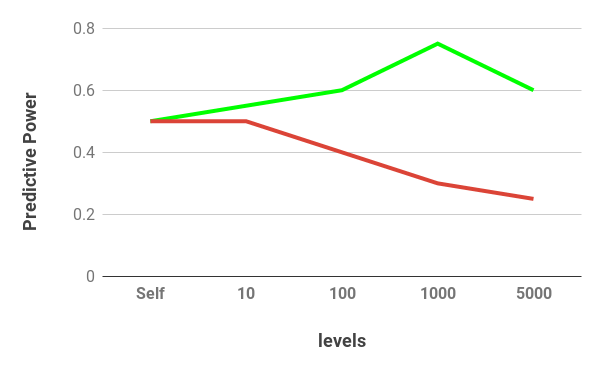
\includegraphics[width=\linewidth]{figs/predictive_power.png}
    \caption{Two hypothetical results about how training set size might effect the efficacy of quality prediction for software projects.}
    \label{fig:predictive_power}
\end{figure}

Petersen and Wohlin~\cite{Petersen2009} argue that for empirical SE, context matters.That is, they would predict that one model  will NOT  cover all  projects and that tools that report  generality  over many software projects need to also know the {\em communities} within which those conclusions   apply. Hence, this work divides into (a)~automated methods for finding sets of projects in the same {\em community}; and (b)~within each {\em community}, find the model what works best. 

The {\em size} of the communities found in this way would have a profound impact on how we should reason about software engineering. Consider the hypothetical results of Figure~\ref{fig:predictive_power}. The \textcolor{ao(english)}{{\bf GREEN}} curve shows some quality predictor that (hypothetically) gets better, the more projects it learns from (i.e. higher levels in the hierarchical cluster). After about 2 levels, the \textcolor{ao(english)}{{\bf GREEN}} curve's growth stops and we would say that community size here was around cluster size in level 1. In this case, while we could not offer a single model that cover {\em all} of SE, we could offer a handful of models, each of which would be relevant to project clusters in that level. Accordingly, we would say that there are many cases where  wisdom from prior projects can be readily applied to guide future projects and (b)~the generality issues raised are not be so pressing.

Now consider the hypothetical \textcolor{red}{{\bf RED}} curve of Figure~\ref{fig:predictive_power}. Here, we see that (hypothetically)  learning from more projects makes quality predictions worse which means the our 10,000 projects break up into ``communities'' of size one. In this case,  (a)~principles about what is ``best practice'' for different software projects would be constantly change (whenever we jump from small community to small community); and (b)~the generality issues would be become open and urgent concerns for the SE analytics community.


\subsection{Related Work}
\label{sec:related}

In this section, we ask ``Why even bother to transfer lessons learned between projects?''. In several recent studies ~\cite{bettenburg2012think, menzies2012local, posnett2011ecological} with readily-available data from SE repositories, numerous authors report the locality effect in SE; i.e. general models outperformed by specialized models localized to particular parts of the data. Menzies et al. showed in their paper about local vs global learning in defect prediction and effort estimation domain that using a rule based learner locality based learning was much effective then rules learned from the global dataset. While Herbold et al.~\cite{herbold2017global} in their study regarding global vs local model for cross-project defect prediction showed evident proof that local models make only a minor difference in comparison to global models. While local can cause conclusion instabilities, global models can miss details which is specific to certain dataset. So in this study, we review the evidence that if it is useful to explore more than just the local data. This evidence falls into four groups:

\textbf{(a) The lesson on big data is that that the {\em more} training data, the {\em better} the learned model.} Vapnik~\cite{vapnik14} discusses examples where models accuracy improves to nearly 100\%, just by training on $10^2$ times as much data. This effect has yet to be seen in SE data~\cite{menzies2013guest} but that might just mean we have yet to use enough training data (hence, this study). 

\textbf{(b) We need to learn from more data since there is very little agreement on what has been learned to far:} Another reason to try generalizing across more SE data is that, among developers, there is little agreement on what many issues relating to software:
\bi
    \item
    According to Passos et al.~\cite{passos11},  developers often  assume that the lessons they learn from a few past projects are general to all their future projects. They comment, ``past experiences were taken into account without much consideration for their context'' ~\cite{passos11}. 
	\item
	J{\o}rgensen \& Gruschke~\cite{Jo09} offer a similar warning. They report that the suppose software engineering ``gurus'' rarely use lessons from past projects to improve their future reasoning and that such poor past advice can be detrimental to new projects.~\cite{Jo09}.
    \item 
    Other studies have shown some widely-held views are   now questionable given new evidence. Devanbu et al. examined responses from 564 Microsoft software developers from around
	the world. They comment programmer beliefs can vary with each project, but do not necessarily
	correspond with actual evidence in that project~\cite{De16}. 
\ei
	
The good news is that, using software analytics, we can correct the above misconceptions. If data mining shows that doing  XYZ is bug prone, then we could  guide developers to avoid XYZ. But will developers listen to us? If they ask ``are we sure  XYZ causes problems?'', can we say that we have mined enough projects to ensure that XYZ is problematic? 

It turns out that developers are not the only ones confused about how various factors influence software projects. Much recent research calls into question  the``established widoms'' of SE field. For example, here is a list of recent conclusions that contradict prior conclusions:

\bi

    \item In stark contrast to  much prior research, pre- and post- release failures are not connected~\cite{fenton2000quantitative};
    
    \item Static code analyzers perform no better than simple statistical predictors~\cite{Fa13}; 
    
    \item The language construct GOTO, as used in contemporary practice, is rarely considered harmful~\cite{nagappan2015empirical};
    
    \item Strongly typed languages are not associated with successful projects~\cite{ray2014large};  
    
    \item Test-driven development is not any better than "test last"~\cite{fucci2017dissection};
    
    \item Delayed issues are not exponentially more expensive to fix~\cite{menzies2017delayed};

\ei

Note that if the reader disputes any of the above, then we ask how would you challenge the items on this list? Where would you get the data, from enough projects, to   successfully refute the above? And where would you get that data? And how would you draw conclusions from that large set?

\textbf{(c) Imported data can be more useful than local data:} Another benefit of  importing data from other projects is that, sometimes, that imported data can be better than the local information. For example, Rees-Jones reports in one study that while building predictors
for Github close time  for open source projects~\cite{rees2017better} using data from other projects performs much better then building models using {\em local learning} (because there is better  information {\em there} than {\em here}).


\textbf{(d) When there is insufficient local data, learning from other projects is very useful:} When developing new software in  novel areas, it is useful to draw on the relevant  experience  from related areas with a larger experience base.This is particularly true when developers are doing something that is novel to them, but has been widely applied elsewhere
For example, Clark and Madachy~\cite{clark15} discuss 65 types of software they see        under-development by the US Defense Department in 2015.   Some of these types are very common (e.g. 22 ground-based communication systems) but other types are very rare (e.g. only  one avionics communication system). (e.g. workers on   flight avionics   might check for lessons learned from ground-based communications). Developers  working in an uncommon area (e.g. avionics communications) might want to transfer in lessons from more common areas (e.g. ground-based communication).


This fuels the art of moving data and/or lessons learned from one project or another is Transfer Learning. This is when there is insufficient data to apply data miners to learn defect predictors, transfer learning can be used to transfer lessons learned from other source projects S to the target project T .

Initial experiments with transfer learning offered very pessimistic results. Zimmermann et al.~\cite{zimmermann2009cross} tried to port models between two web browsers (Internet Explorer and Firefox) and found that cross-project prediction was still not consistent: a model built on Firefox was useful for Explorer, but not vice versa, even though both of them are similar applications. Turhan's initial experimental results were also very negative: given data from 10 projects, training on S = 9 source projects and testing on T = 1 target projects resulted in alarmingly high false positive rates (60\% or more). Subsequent research realized that data had to be carefully sub-sampled and possibly transformed before quality predictors from one source are applied to a target project. Transfer learning can be have two variants - 

\bi
    \item \textbf{Homogeneous Transfer Learning:} This kind of transfer learning operates on source and target data that contain the same attributes.
    
    \item \textbf{Heterogeneous Transfer Learning:} This type of transfer learning operates on source and target data that contain the different attributes.
\ei

Another way of to divide transfer learning is the approach that is followed. There are  2 approaches that is frequently used in many research  - 

\bi
    \item \textbf{Similarity Based Approach:} In this approach we can transfer some/all subset of the rows or columns of data from source to target. For example, the Burak filter~\cite{turhan09} builds its training sets by finding the k = 10 nearest code modules in S for every $ t \in T $. However, the Burak filter suffered from the all too common instability problem (here, whenever the source or target is updated, data miners will learn a new model since different code modules will satisfy the k = 10 nearest neighbor criteria). Other researchers ~\cite{kocaguneli2012, kocaguneli2011find} doubted that a fixed value of k was appropriate for all data. That work recursively bi-clustered the source data, then pruned the cluster sub-trees with greatest ``varianc'' (where the ``variance'' of a sub-tree is the variance of the conclusions in its leaves). This method combined row selection with row pruning (of nearby rows with large variance). Other similarity methods~\cite{Zhang16aa} combine domain knowledge with automatic processing: e.g. data is partitioned using engineering judgment before automatic tools cluster the data. To address variations of software metrics between different projects, the original metric values were discretized by rank transformation according to similar degree of context factors.
    
    \item \textbf{Dimensionality Transformation Based Approach:} In this approach we manipulate the raw source data until it matches the target. An initial attempt on performing transfer learning with Dimensionality transform was undertaken by Ma et al.~\cite{Ma2012} with an algorithm called transfer naive Bayes (TNB). This algorithm used information from all of the suitable attributes in the training data. Based on the estimated distribution of the target data, this method transferred the source information to weight instances the training data. The defect prediction model was constructed using these weighted training data. Nam et al.~\cite{Nam13} originally proposed a transform-based method that used TCA based dimensionality rotation, expansion, and contraction to align the source dimensions to the target. They also proposed a new approach called TCA+, which selected suitable normalization options for TCA, When there are no overlapping attributes (in heterogeneous transfer learning) Nam et al.~\cite{Nam2015} found they could dispense with the optimizer in TCA+ by combining feature selection on the source/target following by a Kolmogorov-Smirnov test to find associated subsets of columns. Other researchers take a similar approach, they prefer instead a canonical-correlation analysis (CCA) to find the relationships between variables in the source and target data~\cite{jing2015heterogeneous}.
\ei

Considering all the attempts at transfer learning sampled above, suggested a surprising lack of consistency in the choice of datasets, learning methods, and statistical measures while reporting results of transfer learning. This issue was addressed by ``Bellwether'' suggested by Krishna et al. ~\cite{krishna2017simpler,krishna16}. which is a simple transfer learning technique is defined in 2- folds namely the Bellwether effect and the Bellwether method:

\bi

    \item \textbf{The Bellwether effect} states that, when a community works on multiple software projects,  then there exists one exemplary project, called the bellwether, which can define predictors for the others.
    
    \item \textbf{The Bellwether method} is where we search for the exemplar bellwether project and construct a transfer learner with it. This transfer learner is then used to predict for effects in future data for that community.

\ei

In their paper Krishna et al. performs experiment with communities of 3, 5 and 10 projects in each, and shows that bellwethers are not rare, their prediction performance is better than local learning, they do fairly well when compared with State of the Art transfer learning methods discussed above and with selection of bellwether shows a consistency for choice of source dataset for transfer learning. This motivated us to use ``Bellwether'' as our choice of method for transfer learning to search for generality in SE datasets. But as per Krishna et al. in order to find bellwether we need to do a $ N*(N-1) $ comparison which is order of $ N^2 $ (N being the number of projects in community). This indeed a very expensive computation. This motivated our study to find generality in SE datasets using a faster Bellwether method. 

Include details about BIRCH and effect of clustering and talk about divide and conquer. 

\section{Data Collection}
\label{sec:Data Collection}

\subsection{Data}
\label{sec:data}

To perform our experiments we choose to work with defect prediction datasets. We use data collected by zhang et al.~\cite{zhang15}. The original data was initially collected by Mockus et al.~\cite{mockus2009amassing} from SourceForge and GoogleCode and was updated till 2010. The dataset contains the full history of about 154K projects that are hosted on SourceForge and 81K projects that are hosted on GoogleCode to the date they were collected. In the original dataset each file contained the revision history and commit logs linked using a unique identified. Although there were 235K projects in the original database, we know from previous literature surveys and experience there were many trivial and non-software development projects. zhang et al. cleaned the dataset using 5 different criteria which resulted in 1385 projects being selected in the final datasets. As part of this experiment we also included few filters to select a subset of 1385 projects, which are useful for our experiment. This eventually gave us a dataset of 697 projects. The filters applied to filter out trivial projects are - 

\bi

    \item \textbf{Programming Languages:} Filtering Out Projects by Programming Languages(only object-oriented i.e *.c, *.cpp, *.cxx, *.cc, *.cs, *.java, and *.pas). This was done as the dataset was collected using a commercial tool, called Understand~\cite{visualize}(which supports the object oriented programming languages) , to compute code metrics. 

    \item \textbf{Projects with a Small Number of Commits:} As small number of commits can mean the projects do not follow a proper SE development process or they are very new, also small number of commits can not provide enough information for computing process metrics and mining defect data. Thus zhang et al. removed any projects with less than 32 commits(25 \% quantile of the number of commits as the threshold).
    
    \item \textbf{Projects with Lifespan Less Than One Year:} zhang et al. collected data in the six-months period using a split date from the first commit and compute process metrics using the change history in the six-months period before the split date. For this reason projects with a lifespan less than one year were filtered out.
    
    \item \textbf{Projects with Limited Defect Data:} For this study defect data was mined using commit messages and bug tracking reports. zhang et al. in their study counted the number of fix-inducing and non-fixing commits from a one-year period and used 152 and 1,689 commits for fix-inducing and non-fixing  respectively for SourceForge. Similarly  92 and 985 commits for GoogleCode. This number was decided by calculating the 75 \% quantile of the number of fix-inducing and non-fixing commits.
    
    \item \textbf{Projects Without Fix-Inducing Commits:} zhang et al. filtered out projects that have no fix-inducing commits during six months as abnormal projects, as projects in defect prediction studies need to contain both defective and non-defective commits.
    
    \item \textbf{Projects with less than 50 rows:} We removed any project with less than 50 rows as they are too small to build a meaningful predictor. 

\ei

\begin{figure}
    \centering
    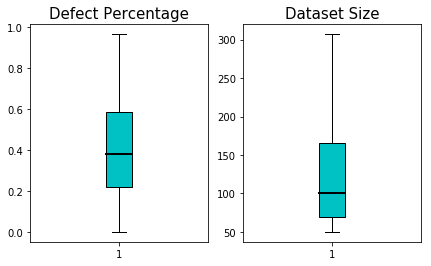
\includegraphics[width=\linewidth]{figs/meta.png}
    \caption{Two hypothetical results about how training set size might effect the efficacy of quality prediction for software projects.}
    \label{fig:meta}
\end{figure}


Along with above filtering criteria, there were few projects which didn't have enough fix-inducing vs non-fixing data points to to create a stratified k=5 fold cross-validation and we removed those projects from the final datasets. These criteria culled 99\% of projects by zhang et al. and culled 54\% of the remaining by our criteria, thus resulted in 697 projects in the final dataset.

From these selected projects, the data was labeled using issue tracking system and commit messages. If a project used issue tracking system for maintaining issue/defect history the data was labeled using that. But as per zhang et al. 42\% of the projects didn't not used issue tracking systems. For these projects labels were created analyzing commit messages by tagging them as fix-inducing commit if commit message matches the following regular expression - 

\begin{center}
\textit{(bug |fix |error |issue |crash |problem |fail |defect |patch)}
\end{center}
 

\subsection{Metric Extraction}
\label{sec:Metric Extraction}

For building any defect predictor we rely on software metrics. Software metrics can be categorized into 3 types according to Xenos \cite{Xenos} distinguishes software metrics as  follows (a) {\em Product metrics} are metrics that are directly related to the product itself, such as code statements, delivered executable, manuals, and strive to measure product quality, or attributes of the product that can be related to product quality. (b) {\em Process metrics} focus on the process of software development and measure process characteristics, aiming to detect problems or to push forward successful practices. Lastly, (c) {\em personnel metrics} (a.k.a. {\em resource metrics}) are those related to the resources required for software development and their performance. The capability, experience of each programmer and communication among all the programmers are related to product quality \cite{wolf2009predicting,de2004sometimes,cataldo2013coordination,cataldo2007coordination}. zhang et al. selected and calculated 21 product and 5 process metrics to build their universal defect prediction model, we will be using the same set of metrics for our study. The product metrics are computed by the Understand tool~\cite{visualize} using the files from the snapshot on the split date of 6 months. The process metrics are computed using the change history in the six-months period before the split date my manual collection of data using scripts. The metrics used in this study are described in table~\ref{tbl:metric}.

\small{
\begin{table}[]
\caption{List of software metrics used in this study}
\label{tbl:metric}
\scriptsize
\begin{tabular}{|p{1cm}|c|l|p{3cm}|}
\hline
\multicolumn{1}{|l|}{Metric}        & \multicolumn{1}{l|}{Metric level} & Metric Name & Metric Description             \\ \hline
\multirow{21}{*}{Product   } & \multirow{6}{*}{File}             & LOC         & Lines of Code                  \\ \cline{3-4} 
                                  &                                   & CL          & Comment Lines                  \\ \cline{3-4} 
                                  &                                   & NSTMT       & Number of Statements           \\ \cline{3-4} 
                                  &                                   & NFUNC       & Number of Functions            \\ \cline{3-4} 
                                  &                                   & RCC         & Ratio Comments to Code         \\ \cline{3-4} 
                                  &                                   & MNL         & Max Nesting Level              \\ \cline{2-4} 
                                  & \multirow{12}{*}{Class}           & WMC         & Weighted Methods per Class     \\ \cline{3-4} 
                                  &                                   & DIT         & Depth of Inheritance Tree      \\ \cline{3-4} 
                                  &                                   & RFC         & Response For a Class           \\ \cline{3-4} 
                                  &                                   & NOC         & Number of Immediate Subclasses \\ \cline{3-4} 
                                  &                                   & CBO         & Coupling Between Objects       \\ \cline{3-4} 
                                  &                                   & LCOM        & Lack of Cohesion in Methods    \\ \cline{3-4} 
                                  &                                   & NIV         & Number of instance variables   \\ \cline{3-4} 
                                  &                                   & NIM         & Number of instance methods     \\ \cline{3-4} 
                                  &                                   & NOM         & Number of Methods              \\ \cline{3-4} 
                                  &                                   & NPBM        & Number of Public Methods       \\ \cline{3-4} 
                                  &                                   & NPM         & Number of Protected Methods    \\ \cline{3-4} 
                                  &                                   & NPRM        & Number of Private Methods      \\ \cline{2-4} 
                                  & \multirow{3}{*}{Methods}          & CC          & McCabe Cyclomatic Complexity   \\ \cline{3-4} 
                                  &                                   & FANIN       & Number of Input Data           \\ \cline{3-4} 
                                  &                                   & FANOUT      & Number of Output Data          \\ \hline
\multirow{5}{*}{Process }  & \multirow{5}{*}{File}             & NREV        & Number of revisions            \\ \cline{3-4} 
                                  &                                   & NFIX        & Number of revisions a file     \\ \cline{3-4} 
                                  &                                   & ADDED LOC    & Lines added                    \\ \cline{3-4} 
                                  &                                   & DELETED LOC  & Lines deleted                  \\ \cline{3-4} 
                                  &                                   & MODIFIED LOC & Lines modified                 \\ \hline
\end{tabular}
\end{table}
}


\section{Experimental Setup}
\label{sec:Experimental}

In this study we try to establish the presence of generality in SE datasets. We do this by analyzing the presence of bellwether incrementally by adding more and more projects and how the bellwether's predictive power changes. In this case to show the presence of generality in SE datasets the predictive power of the bellwether should look like the \textcolor{ao(english)}{GREEN} in figure~\ref{fig:predictive_power}, that is the predictive power of bellwether should increase or remains same, if our results look like the \textcolor{red}{RED} curve, that will show absence of generality in SE datasets.

In order to achieve this we try to explore the \textit{bellwether effect} as mentioned in ~\ref{sec:related}. We know the default \textit{bellwether method} is very expensive ($ O(N^2) $). Thus in this paper we proposes an alternative transfer learning method (BUBBLE), that explores \textit{bellwether effect} by exploring an order of magnitude faster \textit{bellwether method}. Our approach has three key components:

\bi

    \item A feature extractor to find a representation of each project, which will be used for clustering the projects. 
    
    \item A hierarchical clustering model to use the features extracted from previous step to build the hierarchical cluster.
    
    \item A transfer learning model to identify bellwether in the hierarchical cluster.

\ei

BUBBLE employs few different algorithms to complete and compose it's 4 different components - 

\subsection{Feature Subset Selection (FSS)}
\label{subsec:FSS}
To extract features from each dataset, we use a feature selector algorithm called Feature Subset Selection(FSS)~\cite{hall1999correlation,hall1997feature}. Which is a process of identifying and removing as much irrelevant and redundant information as possible. This is achieved using a correlation based feature evolution strategy to evaluate importance of an attribute and a best first search strategy with back tracking that moves through the search space by making local changes to the current feature subset.Here if the path being explored begins to look less promising, the best first search can back-track to a more promising previous subset and continue the search from there. Given enough time, a best first search will explore the entire search space, so it uses a stopping criterion (i.e. no improvement for five consecutive attributes). XXX

\small{
\begin{figure}[]
    \small
     \begin{lstlisting}[mathescape,linewidth=7.5cm,frame=none,numbers=right]
      def CFS(data):
        features = []
        score = -0.000000001
        while True:
            best_feature = None
            for feature in range(data.features):
                features.append(feature)
                temp_score = calculate_corr(data[F])
                if temp_score > score:
                    score = temp_score
                    best_feature = features
                features.pop()
            features.append(best_feature)
            if not improve(score):
                break
        return features
    
    \end{lstlisting} 
    \vspace{-0.2cm}
    \caption{Pseudo-code of Feature Subset Selection}
    \label{fig:GAP_pseudocode} 
    \vspace{-0.3cm}
\end{figure}
}
\subsection{Balanced Iterative Reducing and Clustering using Hierarchies (BIRCH)}
\label{subsec:BIRCH}
To find presence or absence of generality in SE datasets, we need to incrementally check for ``Bellwether'' from smaller to larger community. A community is a set of project which is similar in nature. We use the BIRCH algorithm on our defect prediction dataset to create a hierarchical clustering tree to form these communities. BIRCH~\cite{zhang1996birch} is  a hierarchical clustering algorithm, which has a ability to incrementally and dynamically cluster incoming, multi-dimensional data in an attempt to produce the best quality clustering. BIRCH also has the ability to identify data points that are not part of the underlying pattern effectively identifying outliers. In this study we uses a modified BIRCH algorithm to store additional information regarding each cluster in the clustering feature tree, which help us in the experiment. XXX

\subsection{Synthetic Minority Over-Sampling Technique (SMOTE)}
\label{subsec:SMOTE}

Machine learning models exploits the inherent bias in the dataset to segregate and classify different classes. Hence class imbalance can create major bias towards the majority class when building a machine learning model, thus producing biased model which provides bad classification results. Synthetic Minority Over-Sampling Technique (SMOTE)~\cite{chawla2002smote} is a technique to handle class imbalance by changing the frequency of different classes of the training data. When applied to data, SMOTE sub-samples the majority class (i.e., deletes some examples) while over-sampling the minority class until all classes have the same frequency. In the case of software defect data, the minority class is usually the defective class. During super-sampling, a member of the minority class finds k nearest neighbors. It builds an artificial member of the minority class at some point in-between itself and one of its random nearest neighbors. During that process, some distance function is required which is the \textit{minkowski distance} function.

\subsection{Logistic Regression (LR)}
\label{subsec:LR}

Logistic regression is a statistical machine learning model that in its basic form uses a logistic function to model a binary dependent variable. In this study we use scikit learn's default logistic regression implementation as our learner for building source models and evaluating on target models inside each community. In this study we selected logistic regression, as it is very fast to build in comparison to other more complex learners and its much more comprehensible and explainable in-terms of attributes and their importance. Logistic Regression is widely used in defect prediction domain and have shown promising results both in-term of predictive power and comprehensibility.


\subsection{Bellwether\_0:}
\label{Bellwether}

In this study to compare our novel method to the state of the art method, we uses Krishna et al. 's \textit{bellwether method}. We use all the projects available in the community to perform a $N*(N-1)$ comparison, where N is the number of projects in the community to measure the performance of each project measured on all others on the performance measures mentioned in sec~\ref{sec:Measures}. Following this we use cdom function to select a bellwether project among them. 



\subsection{BUBBLE}
\label{BUBBLE}

BUBBLE is a \textit{bellwether method} algorithm which combines the components described above, to create a fast way to find \textit{bellwether effect}. BUBBLE works in 6 stages - 

    (1) \textbf{Feature Extraction:} In this stage the whole dataset is used to extract feature from each projects. This is done using the FSS algorithm as shown in~\ref{subsec:FSS}. Here each project is sent to the FSS and the FSS returns most suitable features for building models, we do this for every project and that information as a vector (i.e. a vector or length equal to total number of features, where 1 represents a feature being selected ,0 is the other way around) that represents each project. By performing this we have a vector representation of each project in the dataset. BUBBLE uses this information to create the hierarchical clusters to find the communities. We perceive this is a good representation of community, as in this work we try to find community which has similar information distribution according to the attributes. Thus 2 projects with similar features selected have much higher chance of building similar models.
    
    (2) \textbf{Cluster Creation:} After the feature extraction has been done, the data is sent to a modified BIRCH algorithm. The algorithm requires a branching factor (i.e. Maximum number of CF sub-clusters in each node) and threshold value (i.e. when to form a new cluster based on radius). For this experiment we have set the branching factor as 20 and threshold value as 0.5. Using this version of BIRCH algorithm we build the hierarchical cluster, while storing all necessary details about the cluster like parent-child node, data points, level information etc. This stage returns a Clustering Feature Tree (CF Tree) with all those information, which is passed to the next phase of experiment. 
    
    (3) \textbf{Bellwether selection phase 1:} The CF Tree from the last phase is passed to the hierarchical bellwether. In this phase we use \textit{bellwether method} to identify bellwether at the leaf level. Using the CF Tree, we identify the clusters at the leaf level where each cluster represents the smallest community produced by the BIRCH algorithm in the last phase. Here we use the default ``Bellwether'' to perform a $ N*(N-1) $ comparison at each cluster.Here we select each project in the cluster one by one as a source dataset for transfer learning apply SMOTE as mentioned in sec~\ref{subsec:SMOTE} to handle any data imbalance and then use the FSS algorithm to get rid of any unnecessary attributes as mentioned in sec~\ref{subsec:FSS}. This informative and balanced dataset is used to build a LR model as mentioned in sec~\ref{subsec:LR} and we measure the performance of all other projects in the community(cluster). The performance measures that are used are mentioned in sec~\ref{sec:Measures}. To find the bellwether in each community we use cdom function to find the best source dataset among each cluster considering all performance measures. This phase returns a bellwether for each cluster at the leaf level of the CF Tree.
    
    (4) \textbf{Bellwether promotion:} In this phase of the algorithm is an iterative process, here we receive the selected bellwethers from the child clusters of each cluster in the level. This is called the bellwether promotion. Here each parent cluster instead of being represented by all projects within them, they are represented by only the bellwethers in them.  
    
    (5) \textbf{Bellwether selection phase 2:} In this phase instead of finding a bellwether for each cluster at the level by performing a $ N*(N-1) $ comparison, we select the projects which represented as bellwether at the child nodes and then try to find a bellwether among them. So at each cluster at the level we perform a a $ M*(M-1) $ comparison at each cluster where M is the selected bellwether from child clusters. This creates a order of magnitude faster \textbf{bellwether method}. This is again an iterative process, and the end of all the iterations, we will have a bellwether at each cluster at every level. 
    
    (6) \textbf{Bellwether Prediction:} This is the transfer learning phase, when a new project is to evaluated we will use the FSS algorithm to get its features, then use the feature vectors to identify which cluster it belongs and use that cluster's bellwether as the transfer learning model.


To report the finding and results of this study without any bias, we repeat the experiment 20 times by dividing the dataset randomly into train\_1 and test\_1 as a 90-10 split, the projects in train\_1 was used to find the bellwether in each cluster in the CF Tree, and then each project in test\_1 was divide into train\_2 and test\_2 split. We trained a LR model using train\_2 for each project and tested on test\_2, this is represented as self test in this study. We also used the predict stage of the BUBBLE to identify bellwether for each project in test\_1 and tested the performance on test\_2. 


\small{
\begin{figure}[]
    \small
     \begin{lstlisting}[mathescape,linewidth=7.5cm,frame=none,numbers=right]
      def BUBBLE(data):
        project_features = get_features(data)
        cluster_tree = BIRCH(project_features)
        bellwethers = h_bellwether(cluster_tree)
        for project in test_1:
            train_2,test_2 = train_test_split(data[project])
            self_clf = LR(train_2)
            b_clf = find_bellwether(project_features[project])
            self_score = self_clf.predict(test_2)
            bellwether_score = b_clf.predict(test_2)
            results.append([self_score,bellwether_score]) 
        return results
    \end{lstlisting} 
    \vspace{-0.2cm}
    \caption{Pseudo-code of BUBBLE Experiment}
    \label{fig:GAP_pseudocode} 
    \vspace{-0.3cm}
\end{figure}
}

\small{
\begin{figure}[]
    \small
     \begin{lstlisting}[mathescape,linewidth=7.5cm,frame=none,numbers=right]
      def h_bellwether(cluster_tree):
        bellwethers = { }
        def bellwether(list1,list2):
            for source in list1:
                clf = LR(source)
                _list2 = list2.pop(source)
                for dest in _list2:
                    score[source][dest] = clf.predict(dest)
            return best(score.key())
        for level in cluster_tree.levels:
            if level == cluster_tree.max_level:
                for c in cluster_tree[level].clusters:
                    bellwethers[c] = bellwether(c.projects,
                                                c.projects)
            else:
                for c in cluster_tree[level].clusters:
                    child_clusters = c.child
                    _bellwethers = bellwethers[child_clusters]
                    bellwethers[c] = bellwether(_bellwethers,
                                                _bellwethers)
        return bellwethers
    \end{lstlisting} 
    \vspace{-0.2cm}
    \caption{Pseudo-code of Hierarchical Bellwether}
    \label{fig:GAP_pseudocode} 
    \vspace{-0.3cm}
\end{figure}
}

\subsection{Statistical Tests}
\label{stats}

When comparing the results different models in this study, we used a statistical significance test and an effect size test. Significance test are useful for detecting if two populations
differ merely by random noise. Also, effect sizes are useful for checking that two populations differ by more than just a trivial amount. For the significance test,  we use the Scott-Knott procedure  recommended at TSE'13~\cite{mittas2013ranking} and ICSE'15~\cite{ghotra2015revisiting}. This technique recursively bi-clusters a sorted set of numbers. If any two clusters are statistically indistinguishable, Scott-Knott reports them both as one group. Scott-Knott first looks for a break in the sequence that maximizes the expected values in the difference in the means before and after the break.More specifically,  it  splits $l$ values into sub-lists $m$ and $n$ in order to maximize the expected value of differences  in the observed performances before and after divisions. For e.g., lists $l,m$ and $n$ of size $ls,ms$ and $ns$ where $l=m\cup n$, Scott-Knott divides the sequence at the break that maximizes:

\begin{equation}
    E(\Delta)=ms/ls*abs(m.\mu - l.\mu)^2 + ns/ls*abs(n.\mu - l.\mu)^2\
\end{equation}

Scott-Knott then applies some statistical hypothesis test $H$ to check if $m$ and $n$ are significantly different. If so, Scott-Knott then recurses on each division. For this study, our hypothesis test $H$ was a conjunction of the A12 effect size test (endorsed by \cite{arcuri2011practical})  and non-parametric bootstrap sampling \cite{efron94}, i.e., our Scott-Knott divided the data if {\em both} bootstrapping and an effect size test agreed that the division was statistically significant (90\% confidence) and not a ``small'' effect ($A12 \ge 0.6$).

\subsection{Continuous Domination(cdom)}
\label{cdom}
In this study, we compare each project's performance against all other projects in each cluster at the leaf level of the BIRCH as described in section~\ref{BUBBLE} and section~\ref{Bellwether}. We calculate 5 different performance measure for each project as described in section~\ref{sec:Measures}. In order to find a \textit{bellwether effect} in the performances collected we need to combine those 5 performance measures and then rank them using certain criteria. We have used continuous domination (cdom) for this purpose. continuous domination is defined as the set of all points in the objective space that are not dominated by any other points. Unlike Boolean domination, which says a point is dominated by another if and only if the first point is better in every single objective then the second point, continuous domination combines all the objective into a continuous function to compare and then calculate if one point dominates another. Throughout literature continuous domination has proven to be very effective when multiple goals are concerned. The continuous domination function is defined as below, where P is the total population, k is fitness scaling factor and $X\_1$ is the data points we are calculating the domnation for - 

\begin{equation}
    F(X_1) = \sum_{{(X_2\in P) - X_1}} -e^{-I(X_2,X_1)/k}
\end{equation}


\section{Performance Measures}
\label{sec:Measures}

In this section, we introduce the following 5 evaluation measures used in this study to evaluate the performance of machine learning models. Suppose we have a dataset with M changes and N defects. After inspecting 20\% LOC, we inspected m changes and found n defects. Besides, when we find the first defective change, we have inspected k changes. Then the 5 evaluation measures are defined and computed as follows:

(1) \textbf{Recall:} Proportion of inspected defective changes among all the actual defective changes. This is the evaluation measure used by many previous studies~\cite{kamei2012large,yang2016effort,yang2017tlel,xia2016collective,yang2015deep} . They focused on achieving high Recall so that more defective changes could be detected. Recall is computed as: $n/N$.

(2) \textbf{Precision:} Proportion of inspected defective changes among all the inspected changes. A low Precision indicates that developers would encounter more false alarms, which may have negative impact on developers' confidence on the prediction model. Precision is computed as: $n/m$.

(3) \textbf{pf:} Proportion of all suggested defective changes which are not actual defective changes among all the suggested defective changes. A high pf suggests developers will encounter more false alarms which may have negative impact on developers' confidence on the prediction model.

(4) \textbf{popt20:} Proportion number of suggested defective changes among all suggested defective changes, when when 20\% LOC modified by all changes are inspected. A high popt20 indicates that, under the same number of LOC to inspect, developers developers will find more bugs, which means developers will be able to fix more defects with same amount of effort invested. XXX

(5) \textbf{ifa:} Number of Initial False Alarms encountered before we find the first defect. Inspired by previous studies on fault localization~\cite{parnin2011automated,kochhar2016practitioners,xia2016automated}, we assume that if the top-k changes recommended by the model are all false alarms, developers would be frustrated and are not likely to continue inspecting the other changes. For example, Parnin and Orso ~\cite{parnin2011automated} investigated how developers use and benefit from automated debugging tools through a set of human studies. They found that developers would stop inspecting suspicious statements, and turn back to traditional debugging, if they could not get promising results within the first few statements they inspect. ifs is computed as: k.


\section{Results}
\label{sec:results}

\subsection{RQ1: Can we confirm bellwether on large datasets?}
\label{sec:rq1}

In the literature, we saw most of the previous studies has shown bellwether effect with very small datasets. In order to use bellwether to prove presence of generality in SE domain datasets, we first have to showcase the bellwether method suggested by Krishna et al. in their experiment works for large datasets. We use our defect prediction dataset with 697 projects for this purpose. We divide the dataset in train\_1 and test\_1 set and then performed a $ N*(N-1) $ comparison on all the projects in train\_1 set to find a bellwether, and then dividing each project in test\_1 set into train\_2 and test\_2 using a train\_test split. We use the train\_2 to train a LR model and test on test\_2 which is represented as \textit{self\_0} in the figures. Similarly we use the bellwether project from train\_1 to train a LR model and test it on test\_2 which is represented as \textit{bellwether0}. We use statistical tests mentioned in section~\ref{stats} to compare the performance of \textit{self\_0} vs \textit{bellwether0} for all the performance measures mentioned in section~\ref{sec:Measures}, which is shown in figure~\ref{fig:recall}, \ref{fig:precision}, \ref{fig:pf}, \ref{fig:popt20}, \ref{fig:ifa} . It is evident that using the \textit{bellwether method} proposed by Krishna et al. we were able to find bellwether effect in large dataset with 697 projects. This answers this RQ and creates the baseline results for our study. In this RQ1 although we are able to find \textit{bellwether effect}, this method is very expensive, requiring a $ N*(N-1) $ comparison, which in our experimental setup took nearly 75 days of computation on a single core machine. Which takes us to the next research question. 



\subsection{RQ2: How to tame complexity of bellwether?}
\label{sec:rq2}

To tame complexity of bellwether in this RQ, we propose a new bellwether method called ``BUBBLE'' to find bellwether in large datasets. This bellwether method is composed of 6 stages, (a) a feature extraction process to summarize each project into a single representative vector, (b) a hierarchical clustering algorithm, which uses the feature vectors to cluster similar projects into community of increasing size at different levels of cluster, (c) a bellwether selection phase where a $N*(N-1)$ comparison is performed at each leaf level cluster and using a cdom calculation in all the metrics mentioned in~\ref{tbl:metric} a bellwether is selected, (d) a iterative bellwether promotion stage, where bellwether from child clusters are promoted as potential bellwethers at parent cluster, (e) another bellwether selection phase at non-leaf levels, where comparisons are only made among potential bellwethers from leaf node and finally (f) a bellwether prediction phase, which suggests a bellwether based on project similarity when a new project is to be predicted. The details of each phase is mentioned in sec~\ref{BUBBLE}. 

In the \textit{bellwether method} proposed by Krishna et al. if there are N projects in a community it will make $\approx N^2$ comparisons to discover the bellwether. While ``BUBBLE'' different approach to discover bellwether by dividing the data into smaller cluster and finding bellwether among each, here if we assume we have m cluster at leaf level with N projects in each, we will have 
$\approx N^2/m$ comparisons to discover the bellwether which is m times less comparison. Using this process we able to find bellwether in ~1.5 hours, which is order of magnitude faster then the bellwether method proposed by Krishna et al. 

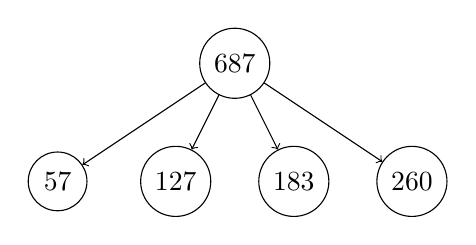
\begin{tikzpicture}[nodes={draw, circle}, ->]
 
    \node{687}
        child { node {57} }
        child { node {127} }
        child { node {183} }
        child { node {260} };
 
\end{tikzpicture}



%%%%%%%%%%%%%%%%%%%%%%%%%%%%%%%%%%%%%%%%%%%%%%%%%%%%%%%%%%%
%%%%%%%%%%%%%%%%%%%%%%%Latex Table%%%%%%%%%%%%%%%%%%%%%%%%%
\begin{figure}[!t]
{\small
{\small \begin{tabular}{llrrc}
\arrayrulecolor{darkgray}
\rowcolor[gray]{.9}  rank & treatment & median & IQR & \\
    1 &      self\_0 &    50 &  86 & \quart{0}{50}{86}{36} \\
    2 &      bellwether0 &    67 &  64 & \quart{36}{67}{64}{33} \\
    2 &      bellwether\_level2 &    67 &  67 & \quart{33}{67}{67}{33} \\
    2 &      bellwether\_level1 &    67 &  62 & \quart{38}{67}{62}{33} \\
    3 &      bellwether\_level0 &    78 &  50 & \quart{50}{78}{50}{22} \\
\end{tabular}}
}
\caption{Recall
}\label{fig:recall}
\end{figure}
%%%%%%%%%%%%%%%%%%%%%%%End Latex Table%%%%%%%%%%%%%%%%%%%%%
%%%%%%%%%%%%%%%%%%%%%%%%%%%%%%%%%%%%%%%%%%%%%%%%%%%%%%%%%%%

%%%%%%%%%%%%%%%%%%%%%%%%%%%%%%%%%%%%%%%%%%%%%%%%%%%%%%%%%%%
%%%%%%%%%%%%%%%%%%%%%%%Latex Table%%%%%%%%%%%%%%%%%%%%%%%%%
\begin{figure}[!t]
{\small
{\small \begin{tabular}{llrrc}
\arrayrulecolor{darkgray}
\rowcolor[gray]{.9}  rank & treatment & median & IQR & \\
    1 &      bellwether\_level0 &    43 &  47 & \quart{20}{43}{47}{24} \\
    1 &      bellwether0 &    44 &  47 & \quart{20}{44}{47}{23} \\
    1 &      bellwether\_level2 &    50 &  51 & \quart{20}{50}{51}{21} \\
    1 &      bellwether\_level1 &    50 &  51 & \quart{20}{50}{51}{21} \\
    1 &      self\_0 &    60 &  83 & \quart{0}{60}{83}{23} \\
\end{tabular}}
}
\caption{Precision
}\label{fig:precision}
\end{figure}
%%%%%%%%%%%%%%%%%%%%%%%End Latex Table%%%%%%%%%%%%%%%%%%%%%
%%%%%%%%%%%%%%%%%%%%%%%%%%%%%%%%%%%%%%%%%%%%%%%%%%%%%%%%%%%

%%%%%%%%%%%%%%%%%%%%%%%%%%%%%%%%%%%%%%%%%%%%%%%%%%%%%%%%%%%
%%%%%%%%%%%%%%%%%%%%%%%Latex Table%%%%%%%%%%%%%%%%%%%%%%%%%
\begin{figure}[!t]
{\small
{\small \begin{tabular}{llrrc}
\arrayrulecolor{darkgray}
\rowcolor[gray]{.9}  rank & treatment & median & IQR & \\
    1 &      self\_0 &    20 &  50 & \quart{0}{20}{50}{30} \\
    2 &      bellwether0 &    50 &  55 & \quart{25}{50}{55}{30} \\
    2 &      bellwether\_level2 &    50 &  54 & \quart{21}{50}{54}{25} \\
    2 &      bellwether\_level1 &    50 &  50 & \quart{25}{50}{50}{25} \\
    3 &      bellwether\_level0 &    67 &  67 & \quart{33}{67}{67}{33} \\
\end{tabular}}
}
\caption{PF
}\label{fig:pf}
\end{figure}
%%%%%%%%%%%%%%%%%%%%%%%End Latex Table%%%%%%%%%%%%%%%%%%%%%
%%%%%%%%%%%%%%%%%%%%%%%%%%%%%%%%%%%%%%%%%%%%%%%%%%%%%%%%%%%

%%%%%%%%%%%%%%%%%%%%%%%%%%%%%%%%%%%%%%%%%%%%%%%%%%%%%%%%%%%
%%%%%%%%%%%%%%%%%%%%%%%Latex Table%%%%%%%%%%%%%%%%%%%%%%%%%
\begin{figure}[!t]
{\small
{\small \begin{tabular}{llrrc}
\arrayrulecolor{darkgray}
\rowcolor[gray]{.9}  rank & treatment & median & IQR & \\
    1 &      bellwether0 &    33 &  21 & \quart{25}{33}{21}{13} \\
    1 &      self\_0 &    33 &  50 & \quart{0}{33}{50}{17} \\
    1 &      bellwether\_level2 &    33 &  20 & \quart{25}{33}{20}{12} \\
    1 &      bellwether\_level0 &    33 &  16 & \quart{27}{33}{16}{10} \\
    1 &      bellwether\_level1 &    33 &  20 & \quart{25}{33}{20}{12} \\
\end{tabular}}
}
\caption{Popt20
}\label{fig:popt20}
\end{figure}
%%%%%%%%%%%%%%%%%%%%%%%End Latex Table%%%%%%%%%%%%%%%%%%%%%
%%%%%%%%%%%%%%%%%%%%%%%%%%%%%%%%%%%%%%%%%%%%%%%%%%%%%%%%%%%


%%%%%%%%%%%%%%%%%%%%%%%%%%%%%%%%%%%%%%%%%%%%%%%%%%%%%%%%%%%
%%%%%%%%%%%%%%%%%%%%%%%Latex Table%%%%%%%%%%%%%%%%%%%%%%%%%
\begin{figure}[!t]
{\small
{\small \begin{tabular}{llrrc}
\arrayrulecolor{darkgray}
\rowcolor[gray]{.9}  rank & treatment & median & IQR & \\
    1 &      bellwether0 &    1 &  4 & \quartx{0}{1}{4}{3} \\
    1 &      self\_0 &    1 &  5 & \quartx{0}{1}{5}{4} \\
    1 &      bellwether\_level2 &    1 &  4 & \quartx{0}{1}{4}{3} \\
    1 &      bellwether\_level0 &    1 &  4 & \quartx{0}{1}{4}{3} \\
    1 &      bellwether\_level1 &    1 &  4 & \quartx{0}{1}{4}{3} \\
\end{tabular}}
}
\caption{IFA
}\label{fig:ifa}
\end{figure}
%%%%%%%%%%%%%%%%%%%%%%%End Latex Table%%%%%%%%%%%%%%%%%%%%%
%%%%%%%%%%%%%%%%%%%%%%%%%%%%%%%%%%%%%%%%%%%%%%%%%%%%%%%%%%%


\subsection{RQ3: Is faster bellwether effective?}
\label{sec:rq3}

In RQ2, we can see using ``BUBBLE'' we are able to find bellwether for a large dataset in order of magnitude faster. This raises the question is  \textit{bellwether method} ``BUBBLE'' as effective as \textit{bellwether method} proposed by krishna et al.? To answer this question in this study we have used the defect prediction dataset with 697 projects and divided the projects randomly into train\_1 and test\_1 as a 90-10 split, the projects in train\_1 was used to find the bellwether in each cluster in the CF Tree as mentioned in sec~\ref{BUBBLE}, and then each project in test\_1 was divide into train\_2 and test\_2 split. We trained a LR model using train\_2 for each project and tested on test\_2 (represented as self\_0), this is represented as self test in this study. We also used the predict stage of the ``BUBBLE'' to identify a bellwether in each level of hierarchical model, for each project in test\_1 and tested the performance on test\_2 (represented as bellwether\_level0, bellwether\_level1, bellwether\_level respectively). Similarly we used the projects in train\_1 to find the bellwether using default bellwether method as mentioned in sec~\ref{Bellwether}, and use that project to build a LR model and test the performance of each project's test\_2 (represented as bellwether0). We compare the performance of each model described above using statistical tests as mentioned in section~\ref{stats} and if 2 models are ranked different that represents their performance is significantly different. We can see from the figure~\ref{fig:recall} that bellwether\_level0 model (i.e. the bellwether discovered by ``BUBBLE'' at level 0) performs best with a median of 78 and IQR of 50. 
We can see from the results in , ~\ref{fig:precision}, ~\ref{fig:pf}, ~\ref{fig:popt20}, ~\ref{fig:ifa}. 


\subsection{RQ4: Should SE uses general methods or cohert based methods?}
\label{sec:rq4}

This RQ is about presence of generality in SE datasets based on the results from ``BUBBLE'' in RQ~\ref{sec:rq1}, RQ~\ref{sec:rq2} and RQ~\ref{sec:rq3}. 

\section{Discussion}
\label{sec:discuss}
What's old is new. Our results 

\section{Threats to Validity}
\label{sec:validity}

As with any large scale empirical study, biases can affect the final
results. Therefore, any conclusions made from this work
must be considered with the following issues in mind:

\bi 

\item \textit{Evaluation Bias}: 
In  RQ1, RQ2 and RQ3 we have shown the performance of local model, hierarchical bellwether models, default bellwether model and compared them using statistical tests on their performance to make conclusion about presence of generality in SE datasets. While those results are true, that conclusion is scoped by the evaluation metrics we used to write this paper. It is possible that, using other measurements, there may well be a difference in these different kinds of projects. This is a matter that needs to be explored in future research.  

    
\item \textit{Construct Validity}: At various places in this report, we made engineering decisions about (e.g.) choice of machine learning models, hierarchical clustering algorithm, selecting feature vectors for each r=project. While those decisions were made using advice from the literature, we acknowledge that other constructs might lead to different conclusions. 

\item \textit{External Validity}: For this study we have relied on data collected by zhang et al.~\cite{zhang15} for their studies. The metrics collected for each project was done using an commercialized tool called ``Understand''. There is a possibility that calculation of metrics or labeling of defective vs non-defective using other tools or methods may result in different outcome. That said, the ``Understand'' is a commercialized tool which has detailed documentation about the metrics calculations and zhang et al. has shared their scripts and process to convert the metrics to usable format and has described the approach to label defects.  

We have relied on issues marked as a `bug' or `enhancement' to count bugs or enhancements, and bug or enhancement resolution times. In Github, a bug or enhancement might not be marked in an issue but in commits. There is also a possibility that the team of that project might be using different tag identifiers for bugs and enhancements. To reduce the impact of this problem, we  did take precautionary step to (e.g.,) include various tag identifiers from Cabot et al.~\cite{cabot2015exploring}. We also took precaution to remove any pull merge requests from the commits to remove any extra contributions added to the hero programmer. 

\item \textit{Statistical Validity}: To increase the validity of our results, we applied two statistical tests, bootstrap and the a12. Hence, anytime in this paper we reported that ``X was different from Y'' then that report was based on both an effect size and a statistical significance test.
 
\item \textit{Sampling Bias}: Our conclusions are based on the 697 projects collected by zhang et al.~\cite{zhang15} for their studies. It is possible that different initial projects would have lead to different conclusions. That said, this sample is very large so we have some confidence that this sample represents an interesting range of projects. As evidence of that, we note that our sampling bias is less pronounced than other ``Bellwether'' studies since we explored.
 
\ei



\section{Conclusion}
\label{sec:concl}

The established wisdom in the literature is to depreciate `

\section{Future Work}
\label{sec:furute}



\section{Acknowledgements}
\label{sec:ack}

The first and second authors conducted this research study as part
of their internship at the industry in Summer, 2017. 


\balance

\bibliographystyle{ACM-Reference-Format}

\bibliography{main}
%
%\documentclass[sigconf]{acmart}
\documentclass[sigconf]{acmart} 
\pdfoutput=1
\usepackage[shortlabels]{enumitem}
\usepackage{balance}
\usepackage{dblfloatfix}

\usepackage{hyperref}
\usepackage{cleveref}
\usepackage{colortbl}
%\usepackage{color}
%\usepackage{booktabs} % For formal tables
%\usepackage{graphicx}
%\usepackage{float}
%\usepackage{listings}
%\usepackage{url}
%\usepackage{comment}
%\usepackage{multirow}
%\usepackage{rotating}
% \usepackage{bigstrut}
% \usepackage{graphics}
% \usepackage{picture}
%\usepackage{cite}

\makeatletter
\let\th@plain\relax
\makeatother


\newcommand{\bi}{\begin{itemize}[leftmargin=0.4cm]}
	\newcommand{\ei}{\end{itemize}}
\newcommand{\be}{\begin{enumerate}[leftmargin=0.4cm]}
	\newcommand{\ee}{\end{enumerate}}


\usepackage{picture}
\newcommand{\quart}[4]{\begin{picture}(100,6)%1
{\color{black}\put(#2,3){\color{red}\circle*{4}}\put(#1,3){\line(1,0){#3}}}\end{picture}}
\newcommand{\quartr}[4]{\begin{picture}(100,6)%1
{\color{black}\put(#2,3){\color{red}\circle*{4}}\put(#1,3){\line(1,0){#3}}}\end{picture}}
\newcommand{\quartx}[4]{\begin{picture}(100,1)%1
{\color{black}\put(\numexpr #2 * 6  \relax,3){\color{red}\circle*{4}}\put(\numexpr #1*6 \relax ,3){\line(1,0){\numexpr #3*6 \relax}}}\end{picture}}

\definecolor{lightgray}{gray}{0.8}
\definecolor{darkgray}{gray}{0.6}
\definecolor{Gray}{gray}{0.85}
\definecolor{Blue}{RGB}{0,29,193}

% \usepackage{tabularx}
% \usepackage{hhline}
% \usepackage[export]{adjustbox}

\definecolor{ao(english)}{rgb}{0.0, 0.5, 0.0}

\definecolor{Gray}{gray}{0.85}
\usepackage{tikz}
\usepackage{framed}
\usepackage[framed]{ntheorem}
\usepackage{multirow}
\usetikzlibrary{shadows}
\usepackage{listings}
\definecolor{MyDarkBlue}{rgb}{0,0.08,0.45} 
\lstset{
    language=Python,
    basicstyle=\sffamily\fontsize{2.5mm}{0.7em}\selectfont,
    breaklines=true,
    prebreak=\raisebox{0ex}[0ex][0ex]{\ensuremath{\hookleftarrow}},
    frame=l,
    keepspaces=false,
    showtabs=false,
    columns=fullflexible,
    showspaces=false,
    showstringspaces=false,
    keywordstyle=\bfseries\sffamily,
    emph={while, for , if ,data, def}, emphstyle=\bfseries\color{blue!50!black},
    stringstyle=\color{green!50!black},
    commentstyle=\color{red!50!black}\it,
    numbers=left,
    captionpos=t,
    escapeinside={\%*}{*)}
}

\theoremclass{Lesson}
\theoremstyle{break}

% inner sep=10pt,
\tikzstyle{thmbox} = [rectangle, rounded corners, draw=black, fill=Gray!40]
\newcommand\thmbox[1]{%
	\noindent\begin{tikzpicture}%
	\node [thmbox] (box){%
		\begin{minipage}{.94\textwidth}%
		\vspace{-0.1cm}#1\vspace{-0.1cm}%
		\end{minipage}%
	};%
	\end{tikzpicture}}

\let\theoremframecommand\thmbox
\newshadedtheorem{lesson}{Result}


% \setcopyright{none}

% % \acmDOI{10.475/123_4}
% % % ISBN
% % \acmISBN{123-4567-24-567/17/08}
% \acmConference[ICSE SEIP'18]{International Conference on Software Engineering, SE in practice track}{May 2018}{Gothenburg, Sweden} 
% \acmYear{2018}
% \copyrightyear{2018}

% \acmPrice{00.00}

%\hyphenation{op-tical net-works semi-conduc-tor}


\begin{document}
%\pagestyle{plain}

\copyrightyear{2018} 
\acmYear{2018} 
\setcopyright{acmcopyright}
\acmConference[ICSE-SEIP '18]{40th International Conference on Software Engineering: Software Engineering in Practice Track}{May 27-June 3, 2018}{Gothenburg, Sweden}
\acmBooktitle{ICSE-SEIP '18: 40th International Conference on Software Engineering: Software Engineering in Practice Track, May 27-June 3, 2018, Gothenburg, Sweden}
\acmPrice{15.00}
\acmDOI{10.1145/3183519.3183549}
\acmISBN{978-1-4503-5659-6/18/05}


\title{BUBBLE}
\subtitle{An Approach to find generality in Software Engineering}

\author{Suvodeep Majumder, Rahul Krishna and Tim Menzies}
\affiliation{Computer Science, NCSU, USA, North Carolina}  
\email{[smajumd3,rkrish11]@ncsu.edu, tim@ieee.org}


\begin{abstract}
Software analytics builds quality prediction models for software projects. After a decade of intensive software analytics there is much disagreement between whether should we use general models that hold over many projects? Or must we use an ever changing set of ideas that are continually adapted to the task at hand? There have many studies that has generated specific results about specific projects~\cite{Bird:2015, menzies2013software} showcasing specificity of SE datasets, while others have argued that those specific local models make only a minor difference in comparison to global models. Experience shows that using local models creates conclusion instability, which results in project managers/developers losing faith in the conclusions about best practices. This can be detrimental to generality, trust,insight, training, and tool developments in SE domain. We have seen from previous studies \textit{bellwether effect}  is an effective way to reduce this conclusion instability, so in this study we propose a novel very fast \textit{bellwether method} algorithm to find a ``Bellwether'' source dataset to show the inherent generality in large SE datasets.

\end{abstract}


% \begin{CCSXML}
% <ccs2012>
% <concept>
% <concept_id>10011007.10011074.10011081.10011082.10011083</concept_id>
% <concept_desc>Software and its engineering~Agile software development</concept_desc>
% <concept_significance>500</concept_significance>
% </concept>
% </ccs2012>
% \end{CCSXML}


% \ccsdesc[500]{Software and its engineering~Agile software development}
\begin{CCSXML}
<ccs2012>
<concept>
<concept_id>10011007.10011074.10011081.10011082.10011083</concept_id>
<concept_desc>Software and its engineering~Agile software 
development</concept_desc>
<concept_significance>500</concept_significance>
</concept>
</ccs2012>
\end{CCSXML}


\ccsdesc[500]{Software and its engineering~Agile software development}


\keywords{Issue, Bug, Commit, Hero, Core, Github, Productivity}

\maketitle

\pagestyle{plain}
%\pagestyle{plain}

\section{Introduction}
How should we reason about SE quality?  Should we use  general models that hold over many projects? Or must we use an ever changing set of ideas that are   continually adapted to the task at hand? 
Or does the truth lie somewhere in-between?  

This is an open and important question. After a decade of intensive research into automated software analytics, what general principles have we learned? While that work has generated specific results about specific projects~\cite{Bird:2015,menzies2013software}, it has failed (so far) to deliver general principles that are demonstrably useful across many projects~\cite{menzies2013guest} (for an example of how {\em more} data can lead to {\em less} general conclusions, see below in {\S}2a).

Is that the best we can do? Are there general principles we can use to guide project management, software standards, education,   tool development, and legislation about software? 
Or is  software engineering some ``patchwork quilt'' of ideas and methods where it only makes sense to reason about specific, specialized, and small sets of related projects? Not to mention, if software was a ``patchwork'' of ideas,then that would  there would be no stable conclusions about what constitutes best practice for software engineering (since those best practices would keep changing as we move from project to project). As discussed in Table~\ref{tbl:why}, such conclusion instability would have detrimental implications for {\em generality, trust, insight, training}, and {\em tool development}.

One  explanation for the limited conclusions (so far) from automated analytics is  {\em how much} data we are using for analysis. A typical software analytics research paper uses less than a few dozen projects  (exceptions: see~\cite{krishna18a, zhao17, agrawal18}). Such small samples can never represent something as diverse as software engineering. Although recent years there have been some studies~\cite{krishna16a,krishna2017simpler,nair19a,mensah18z,mensah2017stratification,mensah2017investigating} to explore generality in Software Engineering. One such process is `` Bellwether ''~\cite{krishna16a,krishna2017simpler,nair19a}, which suggests When local data is scarce, sometimes it is possible to use data collected from other projects either at the local site, or other sites. That is, when building software quality predictors, it might be best to look at more than just the local data. Thus saying there may be data which can be generalized to build models, when local prediction is not possible or useful. However finding such generalizable dataset can be very expensive, as the process suggest to compare each dataset against another to find the generalizable dataset and the previous studies uses small samples to demonstrate the process. 

The central insight of this paper is to find the presence or absence of generality in software engineering, by choosing a suitable source (a.k.a. ``bellwethe'') to learn from, plus a simple transfer learning scheme, which outperforms local learning models. Using this insight, this paper proposes BUBBLE, a novel bellwether based transfer learning scheme, which can identify a suitable source and use it to find near-optimal data source. BUBBLE significantly reduces the cost (in terms of the number of comparisons) to find and build generalized performance models. BUBBLE applies divide and conquer principle by utilizing a hierarchical clustering model to divide the large number of samples in to smaller clusters at every level, and then find and promote bellwether in a bottom-up approach. We evaluate out approach(a.k.a. ``BUBBLE'') using 697 projects and demonstrate that BUBBLE is beneficial.

In a nutshell the contributions of this paper are - 

\bi

\item \textbf{Showing inherent generality in SE datasets:}

\item \textbf{An very fast algorithm to test generality in datasets.} 

\item \textbf{Hierarchical bellwethers as a transfer learner:}


\item \textbf{Richer Replication Package:}

\item \textbf{A new algorithm for transferring data from other projects, unlike prior works it can scale to large datasets.}

\item \textbf{Demo a fast bellwether method which run hours is comparable to a robust method which runs in months.}

\ei

to the best of out knowledge bell/bubble is new high-water mark in qualitative empirical SE. XXX

\section{Background and Related Work}
\label{sec:literature}

\subsection{Motivation}
\label{sec:Motivation}
There are many reasons to seek stable general conclusions in software engineering. If our conclusions about best practices for SE projects keep changing, that will be detrimental to generality, trust, insight, training, and tool development.

\bi

\item \textbf{Generality:} Data science for software engineering cannot be called a ``science'' unless it makes general conclusions that hold across  multiple  projects. If we cannot offer general rules across a large number of software projects, then it is   difficult to demonstrate such generality.

\item \textbf{Trust:} Hassan~\cite{Hassan17} cautions that managers lose faith in software analytics if its models keep changing since  the assumptions used to make prior policy decisions may no longer hold.

\item \textbf{Insight:} Kim et al.~\cite{Kim2016}, say  that the aim of software analytics is to obtain actionable insights that help practitioners accomplish software development goals. For Tan et al.~\cite{tan2016defining}, such   insights  are a core deliverable. Sawyer et al. agrees, saying that  insights are the key driver for businesses to invest in data analytics initiatives~\cite{sawyer2013bi}. Bird, Zimmermann, et al.~\cite{Bird:2015} say that such  insights occur when users reflect, and react, to the output of a model generated via software analytics. But if  new models keep being generated in new projects, then that exhausts the ability of  users to draw insight from  new data.

\item \textbf{Training:} Another concern is what do we train novice software engineers or newcomers to a project? If our models are not stable, then it hard to teach what factors  most influence software quality.

\item \textbf{Tool development:} Further to the last point--- if we are unsure what factors most influence quality, it is difficult to design and implement and deploy tools that can successfully improve that quality.

\ei

\begin{figure}
    \centering
    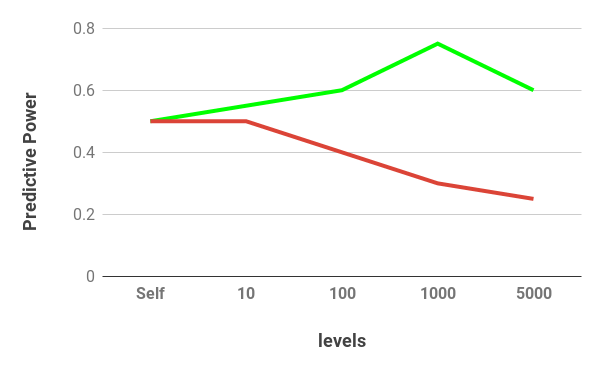
\includegraphics[width=\linewidth]{figs/predictive_power.png}
    \caption{Two hypothetical results about how training set size might effect the efficacy of quality prediction for software projects.}
    \label{fig:predictive_power}
\end{figure}

Petersen and Wohlin~\cite{Petersen2009} argue that for empirical SE, context matters.That is, they would predict that one model  will NOT  cover all  projects and that tools that report  generality  over many software projects need to also know the {\em communities} within which those conclusions   apply. Hence, this work divides into (a)~automated methods for finding sets of projects in the same {\em community}; and (b)~within each {\em community}, find the model what works best. 

The {\em size} of the communities found in this way would have a profound impact on how we should reason about software engineering. Consider the hypothetical results of Figure~\ref{fig:predictive_power}. The \textcolor{ao(english)}{{\bf GREEN}} curve shows some quality predictor that (hypothetically) gets better, the more projects it learns from (i.e. higher levels in the hierarchical cluster). After about 2 levels, the \textcolor{ao(english)}{{\bf GREEN}} curve's growth stops and we would say that community size here was around cluster size in level 1. In this case, while we could not offer a single model that cover {\em all} of SE, we could offer a handful of models, each of which would be relevant to project clusters in that level. Accordingly, we would say that there are many cases where  wisdom from prior projects can be readily applied to guide future projects and (b)~the generality issues raised are not be so pressing.

Now consider the hypothetical \textcolor{red}{{\bf RED}} curve of Figure~\ref{fig:predictive_power}. Here, we see that (hypothetically)  learning from more projects makes quality predictions worse which means the our 10,000 projects break up into ``communities'' of size one. In this case,  (a)~principles about what is ``best practice'' for different software projects would be constantly change (whenever we jump from small community to small community); and (b)~the generality issues would be become open and urgent concerns for the SE analytics community.


\subsection{Related Work}
\label{sec:related}

In this section, we ask ``Why even bother to transfer lessons learned between projects?''. In several recent studies ~\cite{bettenburg2012think, menzies2012local, posnett2011ecological} with readily-available data from SE repositories, numerous authors report the locality effect in SE; i.e. general models outperformed by specialized models localized to particular parts of the data. Menzies et al. showed in their paper about local vs global learning in defect prediction and effort estimation domain that using a rule based learner locality based learning was much effective then rules learned from the global dataset. While Herbold et al.~\cite{herbold2017global} in their study regarding global vs local model for cross-project defect prediction showed evident proof that local models make only a minor difference in comparison to global models. While local can cause conclusion instabilities, global models can miss details which is specific to certain dataset. So in this study, we review the evidence that if it is useful to explore more than just the local data. This evidence falls into four groups:

\textbf{(a) The lesson on big data is that that the {\em more} training data, the {\em better} the learned model.} Vapnik~\cite{vapnik14} discusses examples where models accuracy improves to nearly 100\%, just by training on $10^2$ times as much data. This effect has yet to be seen in SE data~\cite{menzies2013guest} but that might just mean we have yet to use enough training data (hence, this study). 

\textbf{(b) We need to learn from more data since there is very little agreement on what has been learned to far:} Another reason to try generalizing across more SE data is that, among developers, there is little agreement on what many issues relating to software:
\bi
    \item
    According to Passos et al.~\cite{passos11},  developers often  assume that the lessons they learn from a few past projects are general to all their future projects. They comment, ``past experiences were taken into account without much consideration for their context'' ~\cite{passos11}. 
	\item
	J{\o}rgensen \& Gruschke~\cite{Jo09} offer a similar warning. They report that the suppose software engineering ``gurus'' rarely use lessons from past projects to improve their future reasoning and that such poor past advice can be detrimental to new projects.~\cite{Jo09}.
    \item 
    Other studies have shown some widely-held views are   now questionable given new evidence. Devanbu et al. examined responses from 564 Microsoft software developers from around
	the world. They comment programmer beliefs can vary with each project, but do not necessarily
	correspond with actual evidence in that project~\cite{De16}. 
\ei
	
The good news is that, using software analytics, we can correct the above misconceptions. If data mining shows that doing  XYZ is bug prone, then we could  guide developers to avoid XYZ. But will developers listen to us? If they ask ``are we sure  XYZ causes problems?'', can we say that we have mined enough projects to ensure that XYZ is problematic? 

It turns out that developers are not the only ones confused about how various factors influence software projects. Much recent research calls into question  the``established widoms'' of SE field. For example, here is a list of recent conclusions that contradict prior conclusions:

\bi

    \item In stark contrast to  much prior research, pre- and post- release failures are not connected~\cite{fenton2000quantitative};
    
    \item Static code analyzers perform no better than simple statistical predictors~\cite{Fa13}; 
    
    \item The language construct GOTO, as used in contemporary practice, is rarely considered harmful~\cite{nagappan2015empirical};
    
    \item Strongly typed languages are not associated with successful projects~\cite{ray2014large};  
    
    \item Test-driven development is not any better than "test last"~\cite{fucci2017dissection};
    
    \item Delayed issues are not exponentially more expensive to fix~\cite{menzies2017delayed};

\ei

Note that if the reader disputes any of the above, then we ask how would you challenge the items on this list? Where would you get the data, from enough projects, to   successfully refute the above? And where would you get that data? And how would you draw conclusions from that large set?

\textbf{(c) Imported data can be more useful than local data:} Another benefit of  importing data from other projects is that, sometimes, that imported data can be better than the local information. For example, Rees-Jones reports in one study that while building predictors
for Github close time  for open source projects~\cite{rees2017better} using data from other projects performs much better then building models using {\em local learning} (because there is better  information {\em there} than {\em here}).


\textbf{(d) When there is insufficient local data, learning from other projects is very useful:} When developing new software in  novel areas, it is useful to draw on the relevant  experience  from related areas with a larger experience base.This is particularly true when developers are doing something that is novel to them, but has been widely applied elsewhere
For example, Clark and Madachy~\cite{clark15} discuss 65 types of software they see        under-development by the US Defense Department in 2015.   Some of these types are very common (e.g. 22 ground-based communication systems) but other types are very rare (e.g. only  one avionics communication system). (e.g. workers on   flight avionics   might check for lessons learned from ground-based communications). Developers  working in an uncommon area (e.g. avionics communications) might want to transfer in lessons from more common areas (e.g. ground-based communication).


This fuels the art of moving data and/or lessons learned from one project or another is Transfer Learning. This is when there is insufficient data to apply data miners to learn defect predictors, transfer learning can be used to transfer lessons learned from other source projects S to the target project T .

Initial experiments with transfer learning offered very pessimistic results. Zimmermann et al.~\cite{zimmermann2009cross} tried to port models between two web browsers (Internet Explorer and Firefox) and found that cross-project prediction was still not consistent: a model built on Firefox was useful for Explorer, but not vice versa, even though both of them are similar applications. Turhan's initial experimental results were also very negative: given data from 10 projects, training on S = 9 source projects and testing on T = 1 target projects resulted in alarmingly high false positive rates (60\% or more). Subsequent research realized that data had to be carefully sub-sampled and possibly transformed before quality predictors from one source are applied to a target project. Transfer learning can be have two variants - 

\bi
    \item \textbf{Homogeneous Transfer Learning:} This kind of transfer learning operates on source and target data that contain the same attributes.
    
    \item \textbf{Heterogeneous Transfer Learning:} This type of transfer learning operates on source and target data that contain the different attributes.
\ei

Another way of to divide transfer learning is the approach that is followed. There are  2 approaches that is frequently used in many research  - 

\bi
    \item \textbf{Similarity Based Approach:} In this approach we can transfer some/all subset of the rows or columns of data from source to target. For example, the Burak filter~\cite{turhan09} builds its training sets by finding the k = 10 nearest code modules in S for every $ t \in T $. However, the Burak filter suffered from the all too common instability problem (here, whenever the source or target is updated, data miners will learn a new model since different code modules will satisfy the k = 10 nearest neighbor criteria). Other researchers ~\cite{kocaguneli2012, kocaguneli2011find} doubted that a fixed value of k was appropriate for all data. That work recursively bi-clustered the source data, then pruned the cluster sub-trees with greatest ``varianc'' (where the ``variance'' of a sub-tree is the variance of the conclusions in its leaves). This method combined row selection with row pruning (of nearby rows with large variance). Other similarity methods~\cite{Zhang16aa} combine domain knowledge with automatic processing: e.g. data is partitioned using engineering judgment before automatic tools cluster the data. To address variations of software metrics between different projects, the original metric values were discretized by rank transformation according to similar degree of context factors.
    
    \item \textbf{Dimensionality Transformation Based Approach:} In this approach we manipulate the raw source data until it matches the target. An initial attempt on performing transfer learning with Dimensionality transform was undertaken by Ma et al.~\cite{Ma2012} with an algorithm called transfer naive Bayes (TNB). This algorithm used information from all of the suitable attributes in the training data. Based on the estimated distribution of the target data, this method transferred the source information to weight instances the training data. The defect prediction model was constructed using these weighted training data. Nam et al.~\cite{Nam13} originally proposed a transform-based method that used TCA based dimensionality rotation, expansion, and contraction to align the source dimensions to the target. They also proposed a new approach called TCA+, which selected suitable normalization options for TCA, When there are no overlapping attributes (in heterogeneous transfer learning) Nam et al.~\cite{Nam2015} found they could dispense with the optimizer in TCA+ by combining feature selection on the source/target following by a Kolmogorov-Smirnov test to find associated subsets of columns. Other researchers take a similar approach, they prefer instead a canonical-correlation analysis (CCA) to find the relationships between variables in the source and target data~\cite{jing2015heterogeneous}.
\ei

Considering all the attempts at transfer learning sampled above, suggested a surprising lack of consistency in the choice of datasets, learning methods, and statistical measures while reporting results of transfer learning. This issue was addressed by ``Bellwether'' suggested by Krishna et al. ~\cite{krishna2017simpler,krishna16}. which is a simple transfer learning technique is defined in 2- folds namely the Bellwether effect and the Bellwether method:

\bi

    \item \textbf{The Bellwether effect} states that, when a community works on multiple software projects,  then there exists one exemplary project, called the bellwether, which can define predictors for the others.
    
    \item \textbf{The Bellwether method} is where we search for the exemplar bellwether project and construct a transfer learner with it. This transfer learner is then used to predict for effects in future data for that community.

\ei

In their paper Krishna et al. performs experiment with communities of 3, 5 and 10 projects in each, and shows that bellwethers are not rare, their prediction performance is better than local learning, they do fairly well when compared with State of the Art transfer learning methods discussed above and with selection of bellwether shows a consistency for choice of source dataset for transfer learning. This motivated us to use ``Bellwether'' as our choice of method for transfer learning to search for generality in SE datasets. But as per Krishna et al. in order to find bellwether we need to do a $ N*(N-1) $ comparison which is order of $ N^2 $ (N being the number of projects in community). This indeed a very expensive computation. This motivated our study to find generality in SE datasets using a faster Bellwether method. 

Include details about BIRCH and effect of clustering and talk about divide and conquer. 

\section{Data Collection}
\label{sec:Data Collection}

\subsection{Data}
\label{sec:data}

To perform our experiments we choose to work with defect prediction datasets. We use data collected by zhang et al.~\cite{zhang15}. The original data was initially collected by Mockus et al.~\cite{mockus2009amassing} from SourceForge and GoogleCode and was updated till 2010. The dataset contains the full history of about 154K projects that are hosted on SourceForge and 81K projects that are hosted on GoogleCode to the date they were collected. In the original dataset each file contained the revision history and commit logs linked using a unique identified. Although there were 235K projects in the original database, we know from previous literature surveys and experience there were many trivial and non-software development projects. zhang et al. cleaned the dataset using 5 different criteria which resulted in 1385 projects being selected in the final datasets. As part of this experiment we also included few filters to select a subset of 1385 projects, which are useful for our experiment. This eventually gave us a dataset of 697 projects. The filters applied to filter out trivial projects are - 

\bi

    \item \textbf{Programming Languages:} Filtering Out Projects by Programming Languages(only object-oriented i.e *.c, *.cpp, *.cxx, *.cc, *.cs, *.java, and *.pas). This was done as the dataset was collected using a commercial tool, called Understand~\cite{visualize}(which supports the object oriented programming languages) , to compute code metrics. 

    \item \textbf{Projects with a Small Number of Commits:} As small number of commits can mean the projects do not follow a proper SE development process or they are very new, also small number of commits can not provide enough information for computing process metrics and mining defect data. Thus zhang et al. removed any projects with less than 32 commits(25 \% quantile of the number of commits as the threshold).
    
    \item \textbf{Projects with Lifespan Less Than One Year:} zhang et al. collected data in the six-months period using a split date from the first commit and compute process metrics using the change history in the six-months period before the split date. For this reason projects with a lifespan less than one year were filtered out.
    
    \item \textbf{Projects with Limited Defect Data:} For this study defect data was mined using commit messages and bug tracking reports. zhang et al. in their study counted the number of fix-inducing and non-fixing commits from a one-year period and used 152 and 1,689 commits for fix-inducing and non-fixing  respectively for SourceForge. Similarly  92 and 985 commits for GoogleCode. This number was decided by calculating the 75 \% quantile of the number of fix-inducing and non-fixing commits.
    
    \item \textbf{Projects Without Fix-Inducing Commits:} zhang et al. filtered out projects that have no fix-inducing commits during six months as abnormal projects, as projects in defect prediction studies need to contain both defective and non-defective commits.
    
    \item \textbf{Projects with less than 50 rows:} We removed any project with less than 50 rows as they are too small to build a meaningful predictor. 

\ei

\begin{figure}
    \centering
    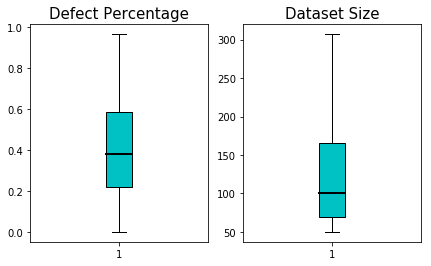
\includegraphics[width=\linewidth]{figs/meta.png}
    \caption{Two hypothetical results about how training set size might effect the efficacy of quality prediction for software projects.}
    \label{fig:meta}
\end{figure}


Along with above filtering criteria, there were few projects which didn't have enough fix-inducing vs non-fixing data points to to create a stratified k=5 fold cross-validation and we removed those projects from the final datasets. These criteria culled 99\% of projects by zhang et al. and culled 54\% of the remaining by our criteria, thus resulted in 697 projects in the final dataset.

From these selected projects, the data was labeled using issue tracking system and commit messages. If a project used issue tracking system for maintaining issue/defect history the data was labeled using that. But as per zhang et al. 42\% of the projects didn't not used issue tracking systems. For these projects labels were created analyzing commit messages by tagging them as fix-inducing commit if commit message matches the following regular expression - 

\begin{center}
\textit{(bug |fix |error |issue |crash |problem |fail |defect |patch)}
\end{center}
 

\subsection{Metric Extraction}
\label{sec:Metric Extraction}

For building any defect predictor we rely on software metrics. Software metrics can be categorized into 3 types according to Xenos \cite{Xenos} distinguishes software metrics as  follows (a) {\em Product metrics} are metrics that are directly related to the product itself, such as code statements, delivered executable, manuals, and strive to measure product quality, or attributes of the product that can be related to product quality. (b) {\em Process metrics} focus on the process of software development and measure process characteristics, aiming to detect problems or to push forward successful practices. Lastly, (c) {\em personnel metrics} (a.k.a. {\em resource metrics}) are those related to the resources required for software development and their performance. The capability, experience of each programmer and communication among all the programmers are related to product quality \cite{wolf2009predicting,de2004sometimes,cataldo2013coordination,cataldo2007coordination}. zhang et al. selected and calculated 21 product and 5 process metrics to build their universal defect prediction model, we will be using the same set of metrics for our study. The product metrics are computed by the Understand tool~\cite{visualize} using the files from the snapshot on the split date of 6 months. The process metrics are computed using the change history in the six-months period before the split date my manual collection of data using scripts. The metrics used in this study are described in table~\ref{tbl:metric}.

\small{
\begin{table}[]
\caption{List of software metrics used in this study}
\label{tbl:metric}
\scriptsize
\begin{tabular}{|p{1cm}|c|l|p{3cm}|}
\hline
\multicolumn{1}{|l|}{Metric}        & \multicolumn{1}{l|}{Metric level} & Metric Name & Metric Description             \\ \hline
\multirow{21}{*}{Product   } & \multirow{6}{*}{File}             & LOC         & Lines of Code                  \\ \cline{3-4} 
                                  &                                   & CL          & Comment Lines                  \\ \cline{3-4} 
                                  &                                   & NSTMT       & Number of Statements           \\ \cline{3-4} 
                                  &                                   & NFUNC       & Number of Functions            \\ \cline{3-4} 
                                  &                                   & RCC         & Ratio Comments to Code         \\ \cline{3-4} 
                                  &                                   & MNL         & Max Nesting Level              \\ \cline{2-4} 
                                  & \multirow{12}{*}{Class}           & WMC         & Weighted Methods per Class     \\ \cline{3-4} 
                                  &                                   & DIT         & Depth of Inheritance Tree      \\ \cline{3-4} 
                                  &                                   & RFC         & Response For a Class           \\ \cline{3-4} 
                                  &                                   & NOC         & Number of Immediate Subclasses \\ \cline{3-4} 
                                  &                                   & CBO         & Coupling Between Objects       \\ \cline{3-4} 
                                  &                                   & LCOM        & Lack of Cohesion in Methods    \\ \cline{3-4} 
                                  &                                   & NIV         & Number of instance variables   \\ \cline{3-4} 
                                  &                                   & NIM         & Number of instance methods     \\ \cline{3-4} 
                                  &                                   & NOM         & Number of Methods              \\ \cline{3-4} 
                                  &                                   & NPBM        & Number of Public Methods       \\ \cline{3-4} 
                                  &                                   & NPM         & Number of Protected Methods    \\ \cline{3-4} 
                                  &                                   & NPRM        & Number of Private Methods      \\ \cline{2-4} 
                                  & \multirow{3}{*}{Methods}          & CC          & McCabe Cyclomatic Complexity   \\ \cline{3-4} 
                                  &                                   & FANIN       & Number of Input Data           \\ \cline{3-4} 
                                  &                                   & FANOUT      & Number of Output Data          \\ \hline
\multirow{5}{*}{Process }  & \multirow{5}{*}{File}             & NREV        & Number of revisions            \\ \cline{3-4} 
                                  &                                   & NFIX        & Number of revisions a file     \\ \cline{3-4} 
                                  &                                   & ADDED LOC    & Lines added                    \\ \cline{3-4} 
                                  &                                   & DELETED LOC  & Lines deleted                  \\ \cline{3-4} 
                                  &                                   & MODIFIED LOC & Lines modified                 \\ \hline
\end{tabular}
\end{table}
}


\section{Experimental Setup}
\label{sec:Experimental}

In this study we try to establish the presence of generality in SE datasets. We do this by analyzing the presence of bellwether incrementally by adding more and more projects and how the bellwether's predictive power changes. In this case to show the presence of generality in SE datasets the predictive power of the bellwether should look like the \textcolor{ao(english)}{GREEN} in figure~\ref{fig:predictive_power}, that is the predictive power of bellwether should increase or remains same, if our results look like the \textcolor{red}{RED} curve, that will show absence of generality in SE datasets.

In order to achieve this we try to explore the \textit{bellwether effect} as mentioned in ~\ref{sec:related}. We know the default \textit{bellwether method} is very expensive ($ O(N^2) $). Thus in this paper we proposes an alternative transfer learning method (BUBBLE), that explores \textit{bellwether effect} by exploring an order of magnitude faster \textit{bellwether method}. Our approach has three key components:

\bi

    \item A feature extractor to find a representation of each project, which will be used for clustering the projects. 
    
    \item A hierarchical clustering model to use the features extracted from previous step to build the hierarchical cluster.
    
    \item A transfer learning model to identify bellwether in the hierarchical cluster.

\ei

BUBBLE employs few different algorithms to complete and compose it's 4 different components - 

\subsection{Feature Subset Selection (FSS)}
\label{subsec:FSS}
To extract features from each dataset, we use a feature selector algorithm called Feature Subset Selection(FSS)~\cite{hall1999correlation,hall1997feature}. Which is a process of identifying and removing as much irrelevant and redundant information as possible. This is achieved using a correlation based feature evolution strategy to evaluate importance of an attribute and a best first search strategy with back tracking that moves through the search space by making local changes to the current feature subset.Here if the path being explored begins to look less promising, the best first search can back-track to a more promising previous subset and continue the search from there. Given enough time, a best first search will explore the entire search space, so it uses a stopping criterion (i.e. no improvement for five consecutive attributes). XXX

\small{
\begin{figure}[]
    \small
     \begin{lstlisting}[mathescape,linewidth=7.5cm,frame=none,numbers=right]
      def CFS(data):
        features = []
        score = -0.000000001
        while True:
            best_feature = None
            for feature in range(data.features):
                features.append(feature)
                temp_score = calculate_corr(data[F])
                if temp_score > score:
                    score = temp_score
                    best_feature = features
                features.pop()
            features.append(best_feature)
            if not improve(score):
                break
        return features
    
    \end{lstlisting} 
    \vspace{-0.2cm}
    \caption{Pseudo-code of Feature Subset Selection}
    \label{fig:GAP_pseudocode} 
    \vspace{-0.3cm}
\end{figure}
}
\subsection{Balanced Iterative Reducing and Clustering using Hierarchies (BIRCH)}
\label{subsec:BIRCH}
To find presence or absence of generality in SE datasets, we need to incrementally check for ``Bellwether'' from smaller to larger community. A community is a set of project which is similar in nature. We use the BIRCH algorithm on our defect prediction dataset to create a hierarchical clustering tree to form these communities. BIRCH~\cite{zhang1996birch} is  a hierarchical clustering algorithm, which has a ability to incrementally and dynamically cluster incoming, multi-dimensional data in an attempt to produce the best quality clustering. BIRCH also has the ability to identify data points that are not part of the underlying pattern effectively identifying outliers. In this study we uses a modified BIRCH algorithm to store additional information regarding each cluster in the clustering feature tree, which help us in the experiment. XXX

\subsection{Synthetic Minority Over-Sampling Technique (SMOTE)}
\label{subsec:SMOTE}

Machine learning models exploits the inherent bias in the dataset to segregate and classify different classes. Hence class imbalance can create major bias towards the majority class when building a machine learning model, thus producing biased model which provides bad classification results. Synthetic Minority Over-Sampling Technique (SMOTE)~\cite{chawla2002smote} is a technique to handle class imbalance by changing the frequency of different classes of the training data. When applied to data, SMOTE sub-samples the majority class (i.e., deletes some examples) while over-sampling the minority class until all classes have the same frequency. In the case of software defect data, the minority class is usually the defective class. During super-sampling, a member of the minority class finds k nearest neighbors. It builds an artificial member of the minority class at some point in-between itself and one of its random nearest neighbors. During that process, some distance function is required which is the \textit{minkowski distance} function.

\subsection{Logistic Regression (LR)}
\label{subsec:LR}

Logistic regression is a statistical machine learning model that in its basic form uses a logistic function to model a binary dependent variable. In this study we use scikit learn's default logistic regression implementation as our learner for building source models and evaluating on target models inside each community. In this study we selected logistic regression, as it is very fast to build in comparison to other more complex learners and its much more comprehensible and explainable in-terms of attributes and their importance. Logistic Regression is widely used in defect prediction domain and have shown promising results both in-term of predictive power and comprehensibility.


\subsection{Bellwether\_0:}
\label{Bellwether}

In this study to compare our novel method to the state of the art method, we uses Krishna et al. 's \textit{bellwether method}. We use all the projects available in the community to perform a $N*(N-1)$ comparison, where N is the number of projects in the community to measure the performance of each project measured on all others on the performance measures mentioned in sec~\ref{sec:Measures}. Following this we use cdom function to select a bellwether project among them. 



\subsection{BUBBLE}
\label{BUBBLE}

BUBBLE is a \textit{bellwether method} algorithm which combines the components described above, to create a fast way to find \textit{bellwether effect}. BUBBLE works in 6 stages - 

    (1) \textbf{Feature Extraction:} In this stage the whole dataset is used to extract feature from each projects. This is done using the FSS algorithm as shown in~\ref{subsec:FSS}. Here each project is sent to the FSS and the FSS returns most suitable features for building models, we do this for every project and that information as a vector (i.e. a vector or length equal to total number of features, where 1 represents a feature being selected ,0 is the other way around) that represents each project. By performing this we have a vector representation of each project in the dataset. BUBBLE uses this information to create the hierarchical clusters to find the communities. We perceive this is a good representation of community, as in this work we try to find community which has similar information distribution according to the attributes. Thus 2 projects with similar features selected have much higher chance of building similar models.
    
    (2) \textbf{Cluster Creation:} After the feature extraction has been done, the data is sent to a modified BIRCH algorithm. The algorithm requires a branching factor (i.e. Maximum number of CF sub-clusters in each node) and threshold value (i.e. when to form a new cluster based on radius). For this experiment we have set the branching factor as 20 and threshold value as 0.5. Using this version of BIRCH algorithm we build the hierarchical cluster, while storing all necessary details about the cluster like parent-child node, data points, level information etc. This stage returns a Clustering Feature Tree (CF Tree) with all those information, which is passed to the next phase of experiment. 
    
    (3) \textbf{Bellwether selection phase 1:} The CF Tree from the last phase is passed to the hierarchical bellwether. In this phase we use \textit{bellwether method} to identify bellwether at the leaf level. Using the CF Tree, we identify the clusters at the leaf level where each cluster represents the smallest community produced by the BIRCH algorithm in the last phase. Here we use the default ``Bellwether'' to perform a $ N*(N-1) $ comparison at each cluster.Here we select each project in the cluster one by one as a source dataset for transfer learning apply SMOTE as mentioned in sec~\ref{subsec:SMOTE} to handle any data imbalance and then use the FSS algorithm to get rid of any unnecessary attributes as mentioned in sec~\ref{subsec:FSS}. This informative and balanced dataset is used to build a LR model as mentioned in sec~\ref{subsec:LR} and we measure the performance of all other projects in the community(cluster). The performance measures that are used are mentioned in sec~\ref{sec:Measures}. To find the bellwether in each community we use cdom function to find the best source dataset among each cluster considering all performance measures. This phase returns a bellwether for each cluster at the leaf level of the CF Tree.
    
    (4) \textbf{Bellwether promotion:} In this phase of the algorithm is an iterative process, here we receive the selected bellwethers from the child clusters of each cluster in the level. This is called the bellwether promotion. Here each parent cluster instead of being represented by all projects within them, they are represented by only the bellwethers in them.  
    
    (5) \textbf{Bellwether selection phase 2:} In this phase instead of finding a bellwether for each cluster at the level by performing a $ N*(N-1) $ comparison, we select the projects which represented as bellwether at the child nodes and then try to find a bellwether among them. So at each cluster at the level we perform a a $ M*(M-1) $ comparison at each cluster where M is the selected bellwether from child clusters. This creates a order of magnitude faster \textbf{bellwether method}. This is again an iterative process, and the end of all the iterations, we will have a bellwether at each cluster at every level. 
    
    (6) \textbf{Bellwether Prediction:} This is the transfer learning phase, when a new project is to evaluated we will use the FSS algorithm to get its features, then use the feature vectors to identify which cluster it belongs and use that cluster's bellwether as the transfer learning model.


To report the finding and results of this study without any bias, we repeat the experiment 20 times by dividing the dataset randomly into train\_1 and test\_1 as a 90-10 split, the projects in train\_1 was used to find the bellwether in each cluster in the CF Tree, and then each project in test\_1 was divide into train\_2 and test\_2 split. We trained a LR model using train\_2 for each project and tested on test\_2, this is represented as self test in this study. We also used the predict stage of the BUBBLE to identify bellwether for each project in test\_1 and tested the performance on test\_2. 


\small{
\begin{figure}[]
    \small
     \begin{lstlisting}[mathescape,linewidth=7.5cm,frame=none,numbers=right]
      def BUBBLE(data):
        project_features = get_features(data)
        cluster_tree = BIRCH(project_features)
        bellwethers = h_bellwether(cluster_tree)
        for project in test_1:
            train_2,test_2 = train_test_split(data[project])
            self_clf = LR(train_2)
            b_clf = find_bellwether(project_features[project])
            self_score = self_clf.predict(test_2)
            bellwether_score = b_clf.predict(test_2)
            results.append([self_score,bellwether_score]) 
        return results
    \end{lstlisting} 
    \vspace{-0.2cm}
    \caption{Pseudo-code of BUBBLE Experiment}
    \label{fig:GAP_pseudocode} 
    \vspace{-0.3cm}
\end{figure}
}

\small{
\begin{figure}[]
    \small
     \begin{lstlisting}[mathescape,linewidth=7.5cm,frame=none,numbers=right]
      def h_bellwether(cluster_tree):
        bellwethers = { }
        def bellwether(list1,list2):
            for source in list1:
                clf = LR(source)
                _list2 = list2.pop(source)
                for dest in _list2:
                    score[source][dest] = clf.predict(dest)
            return best(score.key())
        for level in cluster_tree.levels:
            if level == cluster_tree.max_level:
                for c in cluster_tree[level].clusters:
                    bellwethers[c] = bellwether(c.projects,
                                                c.projects)
            else:
                for c in cluster_tree[level].clusters:
                    child_clusters = c.child
                    _bellwethers = bellwethers[child_clusters]
                    bellwethers[c] = bellwether(_bellwethers,
                                                _bellwethers)
        return bellwethers
    \end{lstlisting} 
    \vspace{-0.2cm}
    \caption{Pseudo-code of Hierarchical Bellwether}
    \label{fig:GAP_pseudocode} 
    \vspace{-0.3cm}
\end{figure}
}

\subsection{Statistical Tests}
\label{stats}

When comparing the results different models in this study, we used a statistical significance test and an effect size test. Significance test are useful for detecting if two populations
differ merely by random noise. Also, effect sizes are useful for checking that two populations differ by more than just a trivial amount. For the significance test,  we use the Scott-Knott procedure  recommended at TSE'13~\cite{mittas2013ranking} and ICSE'15~\cite{ghotra2015revisiting}. This technique recursively bi-clusters a sorted set of numbers. If any two clusters are statistically indistinguishable, Scott-Knott reports them both as one group. Scott-Knott first looks for a break in the sequence that maximizes the expected values in the difference in the means before and after the break.More specifically,  it  splits $l$ values into sub-lists $m$ and $n$ in order to maximize the expected value of differences  in the observed performances before and after divisions. For e.g., lists $l,m$ and $n$ of size $ls,ms$ and $ns$ where $l=m\cup n$, Scott-Knott divides the sequence at the break that maximizes:

\begin{equation}
    E(\Delta)=ms/ls*abs(m.\mu - l.\mu)^2 + ns/ls*abs(n.\mu - l.\mu)^2\
\end{equation}

Scott-Knott then applies some statistical hypothesis test $H$ to check if $m$ and $n$ are significantly different. If so, Scott-Knott then recurses on each division. For this study, our hypothesis test $H$ was a conjunction of the A12 effect size test (endorsed by \cite{arcuri2011practical})  and non-parametric bootstrap sampling \cite{efron94}, i.e., our Scott-Knott divided the data if {\em both} bootstrapping and an effect size test agreed that the division was statistically significant (90\% confidence) and not a ``small'' effect ($A12 \ge 0.6$).

\subsection{Continuous Domination(cdom)}
\label{cdom}
In this study, we compare each project's performance against all other projects in each cluster at the leaf level of the BIRCH as described in section~\ref{BUBBLE} and section~\ref{Bellwether}. We calculate 5 different performance measure for each project as described in section~\ref{sec:Measures}. In order to find a \textit{bellwether effect} in the performances collected we need to combine those 5 performance measures and then rank them using certain criteria. We have used continuous domination (cdom) for this purpose. continuous domination is defined as the set of all points in the objective space that are not dominated by any other points. Unlike Boolean domination, which says a point is dominated by another if and only if the first point is better in every single objective then the second point, continuous domination combines all the objective into a continuous function to compare and then calculate if one point dominates another. Throughout literature continuous domination has proven to be very effective when multiple goals are concerned. The continuous domination function is defined as below, where P is the total population, k is fitness scaling factor and $X\_1$ is the data points we are calculating the domnation for - 

\begin{equation}
    F(X_1) = \sum_{{(X_2\in P) - X_1}} -e^{-I(X_2,X_1)/k}
\end{equation}


\section{Performance Measures}
\label{sec:Measures}

In this section, we introduce the following 5 evaluation measures used in this study to evaluate the performance of machine learning models. Suppose we have a dataset with M changes and N defects. After inspecting 20\% LOC, we inspected m changes and found n defects. Besides, when we find the first defective change, we have inspected k changes. Then the 5 evaluation measures are defined and computed as follows:

(1) \textbf{Recall:} Proportion of inspected defective changes among all the actual defective changes. This is the evaluation measure used by many previous studies~\cite{kamei2012large,yang2016effort,yang2017tlel,xia2016collective,yang2015deep} . They focused on achieving high Recall so that more defective changes could be detected. Recall is computed as: $n/N$.

(2) \textbf{Precision:} Proportion of inspected defective changes among all the inspected changes. A low Precision indicates that developers would encounter more false alarms, which may have negative impact on developers' confidence on the prediction model. Precision is computed as: $n/m$.

(3) \textbf{pf:} Proportion of all suggested defective changes which are not actual defective changes among all the suggested defective changes. A high pf suggests developers will encounter more false alarms which may have negative impact on developers' confidence on the prediction model.

(4) \textbf{popt20:} Proportion number of suggested defective changes among all suggested defective changes, when when 20\% LOC modified by all changes are inspected. A high popt20 indicates that, under the same number of LOC to inspect, developers developers will find more bugs, which means developers will be able to fix more defects with same amount of effort invested. XXX

(5) \textbf{ifa:} Number of Initial False Alarms encountered before we find the first defect. Inspired by previous studies on fault localization~\cite{parnin2011automated,kochhar2016practitioners,xia2016automated}, we assume that if the top-k changes recommended by the model are all false alarms, developers would be frustrated and are not likely to continue inspecting the other changes. For example, Parnin and Orso ~\cite{parnin2011automated} investigated how developers use and benefit from automated debugging tools through a set of human studies. They found that developers would stop inspecting suspicious statements, and turn back to traditional debugging, if they could not get promising results within the first few statements they inspect. ifs is computed as: k.


\section{Results}
\label{sec:results}

\subsection{RQ1: Can we confirm bellwether on large datasets?}
\label{sec:rq1}

In the literature, we saw most of the previous studies has shown bellwether effect with very small datasets. In order to use bellwether to prove presence of generality in SE domain datasets, we first have to showcase the bellwether method suggested by Krishna et al. in their experiment works for large datasets. We use our defect prediction dataset with 697 projects for this purpose. We divide the dataset in train\_1 and test\_1 set and then performed a $ N*(N-1) $ comparison on all the projects in train\_1 set to find a bellwether, and then dividing each project in test\_1 set into train\_2 and test\_2 using a train\_test split. We use the train\_2 to train a LR model and test on test\_2 which is represented as \textit{self\_0} in the figures. Similarly we use the bellwether project from train\_1 to train a LR model and test it on test\_2 which is represented as \textit{bellwether0}. We use statistical tests mentioned in section~\ref{stats} to compare the performance of \textit{self\_0} vs \textit{bellwether0} for all the performance measures mentioned in section~\ref{sec:Measures}, which is shown in figure~\ref{fig:recall}, \ref{fig:precision}, \ref{fig:pf}, \ref{fig:popt20}, \ref{fig:ifa} . It is evident that using the \textit{bellwether method} proposed by Krishna et al. we were able to find bellwether effect in large dataset with 697 projects. This answers this RQ and creates the baseline results for our study. In this RQ1 although we are able to find \textit{bellwether effect}, this method is very expensive, requiring a $ N*(N-1) $ comparison, which in our experimental setup took nearly 75 days of computation on a single core machine. Which takes us to the next research question. 



\subsection{RQ2: How to tame complexity of bellwether?}
\label{sec:rq2}

To tame complexity of bellwether in this RQ, we propose a new bellwether method called ``BUBBLE'' to find bellwether in large datasets. This bellwether method is composed of 6 stages, (a) a feature extraction process to summarize each project into a single representative vector, (b) a hierarchical clustering algorithm, which uses the feature vectors to cluster similar projects into community of increasing size at different levels of cluster, (c) a bellwether selection phase where a $N*(N-1)$ comparison is performed at each leaf level cluster and using a cdom calculation in all the metrics mentioned in~\ref{tbl:metric} a bellwether is selected, (d) a iterative bellwether promotion stage, where bellwether from child clusters are promoted as potential bellwethers at parent cluster, (e) another bellwether selection phase at non-leaf levels, where comparisons are only made among potential bellwethers from leaf node and finally (f) a bellwether prediction phase, which suggests a bellwether based on project similarity when a new project is to be predicted. The details of each phase is mentioned in sec~\ref{BUBBLE}. 

In the \textit{bellwether method} proposed by Krishna et al. if there are N projects in a community it will make $\approx N^2$ comparisons to discover the bellwether. While ``BUBBLE'' different approach to discover bellwether by dividing the data into smaller cluster and finding bellwether among each, here if we assume we have m cluster at leaf level with N projects in each, we will have 
$\approx N^2/m$ comparisons to discover the bellwether which is m times less comparison. Using this process we able to find bellwether in ~1.5 hours, which is order of magnitude faster then the bellwether method proposed by Krishna et al. 

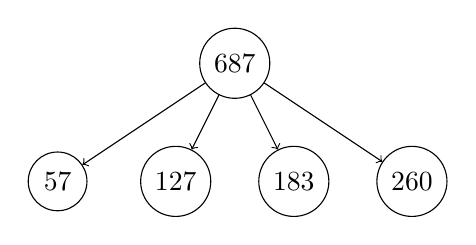
\begin{tikzpicture}[nodes={draw, circle}, ->]
 
    \node{687}
        child { node {57} }
        child { node {127} }
        child { node {183} }
        child { node {260} };
 
\end{tikzpicture}



%%%%%%%%%%%%%%%%%%%%%%%%%%%%%%%%%%%%%%%%%%%%%%%%%%%%%%%%%%%
%%%%%%%%%%%%%%%%%%%%%%%Latex Table%%%%%%%%%%%%%%%%%%%%%%%%%
\begin{figure}[!t]
{\small
{\small \begin{tabular}{llrrc}
\arrayrulecolor{darkgray}
\rowcolor[gray]{.9}  rank & treatment & median & IQR & \\
    1 &      self\_0 &    50 &  86 & \quart{0}{50}{86}{36} \\
    2 &      bellwether0 &    67 &  64 & \quart{36}{67}{64}{33} \\
    2 &      bellwether\_level2 &    67 &  67 & \quart{33}{67}{67}{33} \\
    2 &      bellwether\_level1 &    67 &  62 & \quart{38}{67}{62}{33} \\
    3 &      bellwether\_level0 &    78 &  50 & \quart{50}{78}{50}{22} \\
\end{tabular}}
}
\caption{Recall
}\label{fig:recall}
\end{figure}
%%%%%%%%%%%%%%%%%%%%%%%End Latex Table%%%%%%%%%%%%%%%%%%%%%
%%%%%%%%%%%%%%%%%%%%%%%%%%%%%%%%%%%%%%%%%%%%%%%%%%%%%%%%%%%

%%%%%%%%%%%%%%%%%%%%%%%%%%%%%%%%%%%%%%%%%%%%%%%%%%%%%%%%%%%
%%%%%%%%%%%%%%%%%%%%%%%Latex Table%%%%%%%%%%%%%%%%%%%%%%%%%
\begin{figure}[!t]
{\small
{\small \begin{tabular}{llrrc}
\arrayrulecolor{darkgray}
\rowcolor[gray]{.9}  rank & treatment & median & IQR & \\
    1 &      bellwether\_level0 &    43 &  47 & \quart{20}{43}{47}{24} \\
    1 &      bellwether0 &    44 &  47 & \quart{20}{44}{47}{23} \\
    1 &      bellwether\_level2 &    50 &  51 & \quart{20}{50}{51}{21} \\
    1 &      bellwether\_level1 &    50 &  51 & \quart{20}{50}{51}{21} \\
    1 &      self\_0 &    60 &  83 & \quart{0}{60}{83}{23} \\
\end{tabular}}
}
\caption{Precision
}\label{fig:precision}
\end{figure}
%%%%%%%%%%%%%%%%%%%%%%%End Latex Table%%%%%%%%%%%%%%%%%%%%%
%%%%%%%%%%%%%%%%%%%%%%%%%%%%%%%%%%%%%%%%%%%%%%%%%%%%%%%%%%%

%%%%%%%%%%%%%%%%%%%%%%%%%%%%%%%%%%%%%%%%%%%%%%%%%%%%%%%%%%%
%%%%%%%%%%%%%%%%%%%%%%%Latex Table%%%%%%%%%%%%%%%%%%%%%%%%%
\begin{figure}[!t]
{\small
{\small \begin{tabular}{llrrc}
\arrayrulecolor{darkgray}
\rowcolor[gray]{.9}  rank & treatment & median & IQR & \\
    1 &      self\_0 &    20 &  50 & \quart{0}{20}{50}{30} \\
    2 &      bellwether0 &    50 &  55 & \quart{25}{50}{55}{30} \\
    2 &      bellwether\_level2 &    50 &  54 & \quart{21}{50}{54}{25} \\
    2 &      bellwether\_level1 &    50 &  50 & \quart{25}{50}{50}{25} \\
    3 &      bellwether\_level0 &    67 &  67 & \quart{33}{67}{67}{33} \\
\end{tabular}}
}
\caption{PF
}\label{fig:pf}
\end{figure}
%%%%%%%%%%%%%%%%%%%%%%%End Latex Table%%%%%%%%%%%%%%%%%%%%%
%%%%%%%%%%%%%%%%%%%%%%%%%%%%%%%%%%%%%%%%%%%%%%%%%%%%%%%%%%%

%%%%%%%%%%%%%%%%%%%%%%%%%%%%%%%%%%%%%%%%%%%%%%%%%%%%%%%%%%%
%%%%%%%%%%%%%%%%%%%%%%%Latex Table%%%%%%%%%%%%%%%%%%%%%%%%%
\begin{figure}[!t]
{\small
{\small \begin{tabular}{llrrc}
\arrayrulecolor{darkgray}
\rowcolor[gray]{.9}  rank & treatment & median & IQR & \\
    1 &      bellwether0 &    33 &  21 & \quart{25}{33}{21}{13} \\
    1 &      self\_0 &    33 &  50 & \quart{0}{33}{50}{17} \\
    1 &      bellwether\_level2 &    33 &  20 & \quart{25}{33}{20}{12} \\
    1 &      bellwether\_level0 &    33 &  16 & \quart{27}{33}{16}{10} \\
    1 &      bellwether\_level1 &    33 &  20 & \quart{25}{33}{20}{12} \\
\end{tabular}}
}
\caption{Popt20
}\label{fig:popt20}
\end{figure}
%%%%%%%%%%%%%%%%%%%%%%%End Latex Table%%%%%%%%%%%%%%%%%%%%%
%%%%%%%%%%%%%%%%%%%%%%%%%%%%%%%%%%%%%%%%%%%%%%%%%%%%%%%%%%%


%%%%%%%%%%%%%%%%%%%%%%%%%%%%%%%%%%%%%%%%%%%%%%%%%%%%%%%%%%%
%%%%%%%%%%%%%%%%%%%%%%%Latex Table%%%%%%%%%%%%%%%%%%%%%%%%%
\begin{figure}[!t]
{\small
{\small \begin{tabular}{llrrc}
\arrayrulecolor{darkgray}
\rowcolor[gray]{.9}  rank & treatment & median & IQR & \\
    1 &      bellwether0 &    1 &  4 & \quartx{0}{1}{4}{3} \\
    1 &      self\_0 &    1 &  5 & \quartx{0}{1}{5}{4} \\
    1 &      bellwether\_level2 &    1 &  4 & \quartx{0}{1}{4}{3} \\
    1 &      bellwether\_level0 &    1 &  4 & \quartx{0}{1}{4}{3} \\
    1 &      bellwether\_level1 &    1 &  4 & \quartx{0}{1}{4}{3} \\
\end{tabular}}
}
\caption{IFA
}\label{fig:ifa}
\end{figure}
%%%%%%%%%%%%%%%%%%%%%%%End Latex Table%%%%%%%%%%%%%%%%%%%%%
%%%%%%%%%%%%%%%%%%%%%%%%%%%%%%%%%%%%%%%%%%%%%%%%%%%%%%%%%%%


\subsection{RQ3: Is faster bellwether effective?}
\label{sec:rq3}

In RQ2, we can see using ``BUBBLE'' we are able to find bellwether for a large dataset in order of magnitude faster. This raises the question is  \textit{bellwether method} ``BUBBLE'' as effective as \textit{bellwether method} proposed by krishna et al.? To answer this question in this study we have used the defect prediction dataset with 697 projects and divided the projects randomly into train\_1 and test\_1 as a 90-10 split, the projects in train\_1 was used to find the bellwether in each cluster in the CF Tree as mentioned in sec~\ref{BUBBLE}, and then each project in test\_1 was divide into train\_2 and test\_2 split. We trained a LR model using train\_2 for each project and tested on test\_2 (represented as self\_0), this is represented as self test in this study. We also used the predict stage of the ``BUBBLE'' to identify a bellwether in each level of hierarchical model, for each project in test\_1 and tested the performance on test\_2 (represented as bellwether\_level0, bellwether\_level1, bellwether\_level respectively). Similarly we used the projects in train\_1 to find the bellwether using default bellwether method as mentioned in sec~\ref{Bellwether}, and use that project to build a LR model and test the performance of each project's test\_2 (represented as bellwether0). We compare the performance of each model described above using statistical tests as mentioned in section~\ref{stats} and if 2 models are ranked different that represents their performance is significantly different. We can see from the figure~\ref{fig:recall} that bellwether\_level0 model (i.e. the bellwether discovered by ``BUBBLE'' at level 0) performs best with a median of 78 and IQR of 50. 
We can see from the results in , ~\ref{fig:precision}, ~\ref{fig:pf}, ~\ref{fig:popt20}, ~\ref{fig:ifa}. 


\subsection{RQ4: Should SE uses general methods or cohert based methods?}
\label{sec:rq4}

This RQ is about presence of generality in SE datasets based on the results from ``BUBBLE'' in RQ~\ref{sec:rq1}, RQ~\ref{sec:rq2} and RQ~\ref{sec:rq3}. 

\section{Discussion}
\label{sec:discuss}
What's old is new. Our results 

\section{Threats to Validity}
\label{sec:validity}

As with any large scale empirical study, biases can affect the final
results. Therefore, any conclusions made from this work
must be considered with the following issues in mind:

\bi 

\item \textit{Evaluation Bias}: 
In  RQ1, RQ2 and RQ3 we have shown the performance of local model, hierarchical bellwether models, default bellwether model and compared them using statistical tests on their performance to make conclusion about presence of generality in SE datasets. While those results are true, that conclusion is scoped by the evaluation metrics we used to write this paper. It is possible that, using other measurements, there may well be a difference in these different kinds of projects. This is a matter that needs to be explored in future research.  

    
\item \textit{Construct Validity}: At various places in this report, we made engineering decisions about (e.g.) choice of machine learning models, hierarchical clustering algorithm, selecting feature vectors for each r=project. While those decisions were made using advice from the literature, we acknowledge that other constructs might lead to different conclusions. 

\item \textit{External Validity}: For this study we have relied on data collected by zhang et al.~\cite{zhang15} for their studies. The metrics collected for each project was done using an commercialized tool called ``Understand''. There is a possibility that calculation of metrics or labeling of defective vs non-defective using other tools or methods may result in different outcome. That said, the ``Understand'' is a commercialized tool which has detailed documentation about the metrics calculations and zhang et al. has shared their scripts and process to convert the metrics to usable format and has described the approach to label defects.  

We have relied on issues marked as a `bug' or `enhancement' to count bugs or enhancements, and bug or enhancement resolution times. In Github, a bug or enhancement might not be marked in an issue but in commits. There is also a possibility that the team of that project might be using different tag identifiers for bugs and enhancements. To reduce the impact of this problem, we  did take precautionary step to (e.g.,) include various tag identifiers from Cabot et al.~\cite{cabot2015exploring}. We also took precaution to remove any pull merge requests from the commits to remove any extra contributions added to the hero programmer. 

\item \textit{Statistical Validity}: To increase the validity of our results, we applied two statistical tests, bootstrap and the a12. Hence, anytime in this paper we reported that ``X was different from Y'' then that report was based on both an effect size and a statistical significance test.
 
\item \textit{Sampling Bias}: Our conclusions are based on the 697 projects collected by zhang et al.~\cite{zhang15} for their studies. It is possible that different initial projects would have lead to different conclusions. That said, this sample is very large so we have some confidence that this sample represents an interesting range of projects. As evidence of that, we note that our sampling bias is less pronounced than other ``Bellwether'' studies since we explored.
 
\ei



\section{Conclusion}
\label{sec:concl}

The established wisdom in the literature is to depreciate `

\section{Future Work}
\label{sec:furute}



\section{Acknowledgements}
\label{sec:ack}

The first and second authors conducted this research study as part
of their internship at the industry in Summer, 2017. 


\balance

\bibliographystyle{ACM-Reference-Format}

\bibliography{main}
%\input{main.bbl} 
\end{document} 
\end{document} 
\end{document} 
\end{document}